\documentclass[british,titlepage,oneside]{ntnuthesis}

\title{Stuff}
\shorttitle{Stuff Short}
\author{Emil Martens}
\shortauthor{CoPCSE$@$NTNU}
\date{Spring 2023}

\addbibresource{thesis.bib}


% --------------------
% ----- Commands -----
% --------------------
\newcommand{\code}[1]{\mintinline{text}{#1}\xspace}
\newcommand{\todo}{\textcolor{red}{Todo}\xspace}
\newcommand{\review}{}
% \newcommand{\review}{\textcolor{green}{Draft Complete}\\}
\newcommand{\done}{}
% \newcommand{\done}{\textcolor{olive}{Done}\\}

% From https://www.overleaf.com/learn/latex/Glossaries

\makeglossaries


\setabbreviationstyle[acronym]{long-postshort-user}
\glssetcategoryattribute{acronym}{nohyperfirst}{true}

\setabbreviationstyle{short-nolong}

\renewcommand*{\glsxtruserparen}[2]{%
    \glsxtrfullsep{#2}% space between long part and parenthetical material
    (\glshyperlink[#1]{#2})%
}


\newglossaryentry{jtop}{name=jtop,description={A tool for monitoring the Jetson Nano}}
\newglossaryentry{gigev}{name=GigE Vision,description={\todo}}
\newglossaryentry{jetpack}{name=JetPack,description={\todo}}
\newglossaryentry{jetlinux}{name=NVIDIA Jetson Linux,description={\todo}}
\newglossaryentry{debayer}{name=Debayer,description={\todo}}
\newglossaryentry{igpu}{name=iGPU,description={\todo}}
\newglossaryentry{dgpu}{name=dGPU,description={\todo}}
\newglossaryentry{swap}{name=SWAP,description={\todo}}
\newglossaryentry{tegra}{name=Tegra,description={\todo}}
\newglossaryentry{websocket}{name=WebSocket,description={\todo}}
\newglossaryentry{ide}{name=IDE,description={\todo}}
\newglossaryentry{vscode}{name=Visual Studio Code,description={\todo}}
\newglossaryentry{jinja}{name=Jinja2,description={\todo}}
\newglossaryentry{deepstream}{name=DeepStream,description={\todo}}
\newglossaryentry{f9p}{name=F9P,description={\todo}}
\newglossaryentry{nforum}{name=NVIDIA Developer Forum,description={\todo}}
\newglossaryentry{jetsonclocks}{name=jetson\_clocks,description={\todo}}
\newglossaryentry{nvpmodel}{name=nvpmodel,description={\todo}}
\newglossaryentry{volta}{name=Volta GPU,description={\todo}}

% --------------------
% ----- Acronyms -----
% --------------------

\newacronym{phd}{PhD}{philosophiae doctor}
\newacronym{gcd}{GCD}{Greatest Common Divisor}
\newacronym{imu}{IMU}{Inertial Measurement Unit}
\newacronym{ssd}{SSD}{Solid State Drive}
\newacronym{mtu}{MTU}{Maximum Transmission Unit}
\newacronym{skb}{SKB}{Socket Kernel Buffers}
\newacronym{ram}{RAM}{Random Acces Memory}
\newacronym{rpf}{RPF}{Reverse Path Filtering}
\newacronym{lla}{LLA}{Link-Local Addresses}
\newacronym{dhcp}{DHCP}{Dynamic Host Configuration Protocol}
\newacronym{pps}{PPS}{Pulse Per Second}
\newacronym{ntpd}{NTPD}{Network Time Protocol Daemon}
\newacronym{utc}{UTC}{Coordinated Universal Time}
\newacronym{wsl}{WSL}{Windows Subsystem for Linux}
\newacronym{cfa}{CFA}{Color Filter Array}
\newacronym{gpu}{GPU}{Graphics Processing Unit}
\newacronym{cpu}{CPU}{Central Processing Unit}
\newacronym{asic}{ASIC}{Application Specific Integrated Circuit}
\newacronym{npu}{NPU}{Neural Processing Unit}
\newacronym{fpga}{FPGA}{Field Programmable Gate Array}
\newacronym{isp}{ISP}{Image Signal Processor}
\newacronym{dla}{DLA}{Deep Learning Accelerator}
\newacronym{nvenc}{NVENC}{NVIDIA Multi-Standard Video Encoder}
\newacronym{cuda}{CUDA}{ompute Unified Device Architecture}
\newacronym{simt}{SIMT}{Single Instruction Multiple Threads}
\newacronym{adc}{ADC}{Analog to Digital Converter}
\newacronym{hpc}{HPC}{High Performance Computing}
\newacronym{ai}{AI}{Artificial Intelligence}
\newacronym{gui}{GUI}{Graphical User Interface}
\newacronym{ssh}{SSH}{Secure Shell}
\newacronym{js}{JS}{JavaScript}
\newacronym{sdk}{SDK}{Software Development Kit}
\newacronym{api}{API}{Application Programming Interface}
\newacronym{os}{OS}{Operating System}
\newacronym{rtos}{RTOS}{Real-Time Operating System}
\newacronym{ptp}{PTP}{Precision Time Protocol}
\newacronym{emmc}{eMMC}{Embedded Multi-Media Card}
\newacronym{mhc}{MHC}{Malvar, He, and Cutler}
\glsaddall

\glsunset{cpu}
\glsunset{gpu}

% --------------------
% ----- Shortcuts ----
% --------------------
\newcommand{\nvidia}{NVIDIA\xspace}
\newcommand{\jetson}{Jetson\xspace}
\newcommand{\sr}{Sensor Rig\xspace}
\newcommand{\jx}{Xavier\xspace}
\newcommand{\jo}{Orin\xspace}
\newcommand{\cam}{Triton Polarizin Camera\xspace}
\newcommand{\cams}{Triton Polarizin Cameras\xspace}
\newcommand{\lucid}{Lucid Vision\xspace}
\newcommand{\todo}{TODO\xspace}
\newcommand{\cuda}{CUDA\xspace}
\newcommand{\halftwo}{\_\_half2\xspace}
\newcommand{\preproject}{preproject\xspace}
\newcommand{\master}{master\xspace}
\newcommand{\py}{Python\xspace}
\newcommand{\cpu}{\gls{gpu}\xspace}
\newcommand{\gpu}{\gls{cpu}\xspace}
\newcommand{\gui}{GUI\xspace}
\newcommand{\dash}{Plotly Dash\xspace}
 % add glossary and acronym lists before document
% \oneside
% 
\emergencystretch=1em

\begin{document}
\tableofcontents
% \listoffigures
% \listoftables
% \lstlistoflistings
\pagebreak

\chapter*{Abstract}

Data-driven models have emerged as a promising area of research in the field of \glspl{asv}.
These models have the potential to interpret sensor data and enhance situational awareness.
However, their effectiveness heavily relies on large quantities of high-quality data for training, testing, and validation purposes.

In this \master, I have completed the development of a human-operable \sr for collecting high-quality data in maritime environments.
The \sr is IP67 rated and has two polarization cameras, an \gls{imu}, and two \gls{gnss} receivers, all synchronized to UTC.
The \sr also exposes two additional $1Gb/s$ Ethernet ports with PoE, enabling the connection of additional sensors.

A significant technical achievement in this \master has been to leverage \gls{cuda} and GStreamer for on-the-fly hardware-accelerated video compression on the Jetson Xavier, significantly extending the recording time.
In addition, ergonomic hardware enhancements have been incorporated, along with a new web-based user interface, streamlining the data acquisition process.
Finally, several small data sets were captured in the field to demonstrate the capabilities of the sensor rig as a data collection platform.

This new low-threshold approach to acquiring high-quality data is a strong foundation for my future Ph.D. work and has garnered attention from external entities.
Orders have been placed for the necessary components to create a second \sr, and discussions with external parties for funding a third \sr are currently underway.
These developments demonstrate the positive reception of the \sr and the demand for such a system.


\chapter*{Preface}

This \master's thesis is part of my integrated Ph.D. program at NTNU, where I focus on enhancing multi-sensor detection for \gls{asv}.

Throughout this project, I have had the opportunity to explore diverse topics despite having limited prior experience. The process of learning new things has been enjoyable, albeit challenging at times, and it has inevitably resulted in some technical debt.

I am grateful to several individuals who have provided technical, academic, and emotional support during this journey. Firstly, I would like to express my gratitude to my supervisor, Annette Stahl, for her guidance and proofreading of the final drafts. Additionally, my co-supervisors, Edmund Førland Brekke and Rudolf Mester, have offered valuable feedback throughout the semester. My colleagues at Nyhavna have been wonderful discussion partners and formidable opponents in ping pong matches.

I would like to extend my heartfelt thanks to my family for their unwavering support and their strict reminders to enjoy the sun outside the office.
Finally and most importantly, I would like to thank my soon-to-be wife, Tale Søfting, for her patience and warm hugs when I returned home from long days full of segfaults and compilation errors.





\chapter{Introduction}

\section{Motivation}
Current data sets are often generated through extensive experiments utilizing full-scale systems such as MilliAmpere.
While these experiments are necessary for specific research purposes, the cost-benefit ratio may not be proportional when the primary goal is collecting sensor data.

Recognizing the challenge at hand, I embarked on the development of human operable \sr during my preproject.
The objective was to develop a lightweight \sr that addressed common challenges such as synchronization and pose estimation, paving the way for a low threshold approach to high quality data acquisition.

While most of the hardware and electronics were completed during the preproject, much remained including the challenge of developing a software stack that can effectively manage the large amount of custom raw data produced by the two polarization cameras.




The motivation behind this project stems from my pursuit of an integrated Ph.D.
program, where I will focus on investigating the potential enhancements in detection capabilities for Autonomous Surface Vessels (ASVs) through the integration of data from various sensors, such as lidars and specialized cameras.
This research will heavily involve machine learning techniques, necessitating a significant amount of training data.
Since I will be exploring new sensor combinations, existing datasets alone cannot fulfill the requirements.
Hence, there is a need for a framework that enables the collection of new data, with a preference for a low threshold approach.
Therefore, the development of this sensor rig becomes imperative.


\begin{figure}
    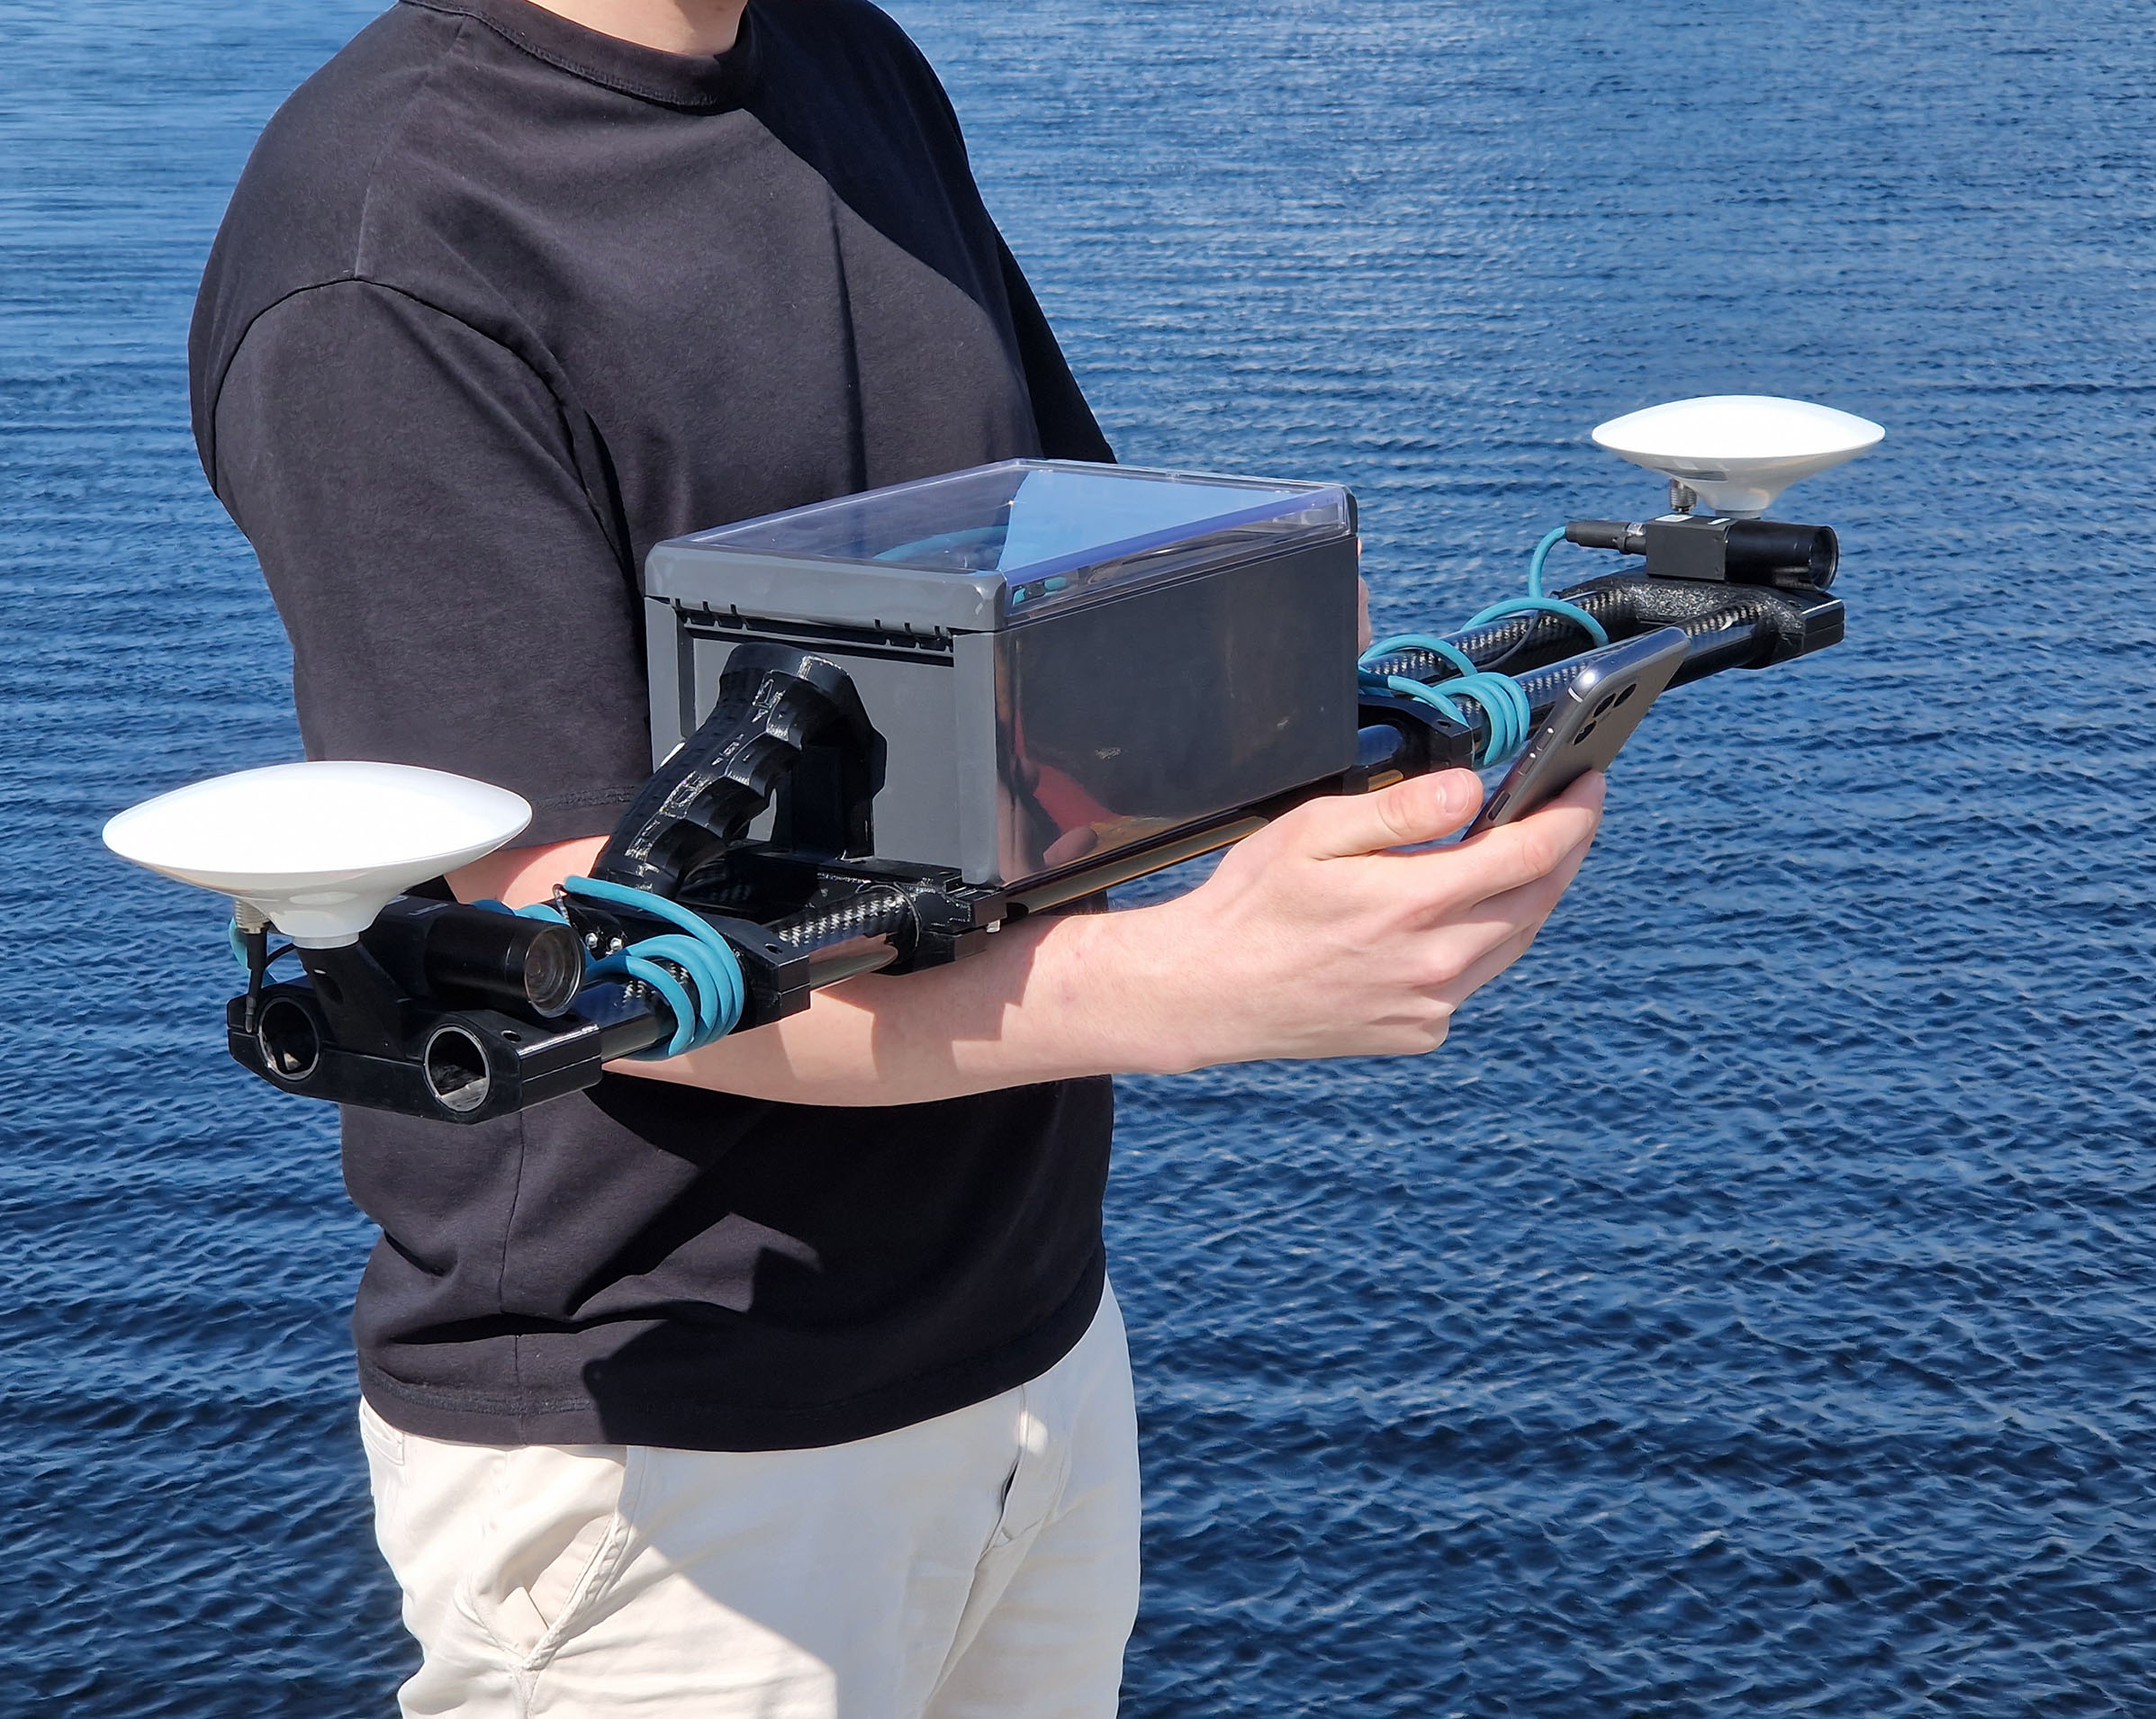
\includegraphics[width=\textwidth]{figures/frontpage.jpg}
    \caption{The Sensor Rig}
\end{figure}
\section{TODO}
Explain how this project is a bit all over the place but show how it ties together with a full page figure.


\section{Motivation}
A significant amout of work was put into enabling on the fly compression of the videostreams from the \sr.
That is the ability to compress the video data as it is being recorded, and storing the compressed data on disk.

The cameras on the \sr produce roughly $2Gb/s$ of data.
Aditionally, the \gls{imu} and \gls{gnss} produce data, but amount is neglible compared with the cameras.
At this rate it infeasable to record long datasets as almost a terrabyte of data is produced every hour.
\begin{align}
    \frac{1TB}{2Gb/s}  = \frac{8Tb}{2Gb/s} = 4000s \approx 1h + 7min
\end{align}

It is reasonable to say that a much easer option is to buy \gls{ssd} with a capacity up to 8TB \cite{CorsairMP600PRO}, enabling roughly 9 hours of recording.
One reason this
\cite{microntechnologyMicron2300SSD2020}


\subsection{Limited write speed}
One issue when storing the raw data at first was that the \jx was not able to write to the disk fast to the installed \gls{ssd}.
The write speed was tested using:
\begin{minted}[linenos=false]{bash}
    sudo dd if=/dev/zero of=./testfile bs=8k count=100k conv=fdatasync
\end{minted}
which repeatedly reported write speeds just below $2Gb/s$ (250MB).
This is weird, as the \gls{ssd} has a write speed of $2.7GB/s$, but other people have faced similar issues on the \jx \cite{microntechnologyMicron2300SSD2020} \cite{dtyuImbalancedPerformanceRead2018}.
This is probably fixable, but provides further motivation to enable on the fly compression


\subsection{Integration with other systems}
The main intended purpose of the \sr is to be carried around by a human operator and

\subsection{Streaming to external devices}
Having a


\section{Challenges}
The main challenge in this project has been to design a system that can effectively manage the large amount of raw data produced by the two cameras.
Each camera features a 5.0MP sensor configured to capture 10-bit raw images 16 times every second \cite{lucidvisionlabsTriton0MPPolarization}.
To put this into perspective, a single frame contains more data than what is needed to store the entire collection of William Shakespeare's works in plain text \cite{projectgutenbergCompleteWorksWilliam1994}.

If the output from these cameras were stored directly to disk, almost a Terabyte of data would be generated every hour, making it infeasible to collect long term data sets.


\section{Outline}
Creating the \sr has been a large undertaking and I have worked on wide variety of different topics including ergonomic hardware design, full stack web development, kernel compilation and low level optimizations in CUDA.
The only thing that is consistent between all the different parts is that they are performed in order to acheive the goal of creating a human operable soensor rig for high quality data collection.










The first, and most extensive part is the software development requiered to collect and compress the data from the \sr in real time.
As this has been the main focus of the project and also is what is most relevant, the first five chapters are dedicated to this.
Following this

\paragraph{Chapter \ref{chap:programming_theory}: Real time programming on Jetson Xavier}
This chapter provides an overview of the theoretical background necessary to achieve real-time performance on the \jx platform.
It covers topics such as real-time programming theory, performance considerations for heterogeneous systems, and a brief introduction to the CUDA programming model.

\paragraph{Chapter \ref{chap:cameras}: Polarization Cameras}
This chapter explains how interaction with the camera is acheived, how they are configured and how various the network adapters have been configured to acheive $2Gb/s$ throughput from the \cams.

\paragraph{Chapter \ref{chap:debayer}: Efficient processing of raw image bitstream in CUDA}
To make it possible to compress the video streams, the raw data has to be transformed into a format that can be processed by the \gls{h265} encoder.
This chapter explains how this is acheived in real time using CUDA.

\paragraph{Chapter \ref{chap:gstreamer}: Video Compression using GStreamer}
\gls{gstreamer} is a powerful framework for processing video streams.
This chapter explains how it is used to compress the video streams in real time using hardware accelration on the \jx.

\paragraph{Chapter \ref{chap:pipeline}: Pipeline Assembly in Python}
\todo

\subsection{Web interface for control and monitoring}

\paragraph{Chapter \ref{chap:gui}: Web Interface to Control, Monitor and Stream Video}
A web application was developed to enabling real time control and monitoring of the \sr and its video streams.
This allows anyone with a smartphone to operate the \sr without any prior training or technical knowledge.


\paragraph{Chapter \ref{chap:flashing_xavier}: Compiling Jetson Linux with PPS}
In order to get the the \gls{gstreamer} pipeline working, it was necessary to update the operating system to a newer version.
As a \gls{pps} signal is used to synchronize the clock on the \jx to \gls{utc}, it was necessary to compile the kernel with support for this, which turned out to be a non-trivial task demanding a systematic approach.

\paragraph{Chapter \ref{chap:hardware}: Improving the Hardware}
After the \preproject most of the hardware was already in place, but some parts were missing.
I applied for, and got, funding to purchase a new 3D printer to enable an iterateive design process.
With this in place custom ergonomic carry handles, new combined camera and antenna mounts and other minor parts were designed and 3D-printed.

\paragraph{Chapter \ref{chap:results}: Results}


\paragraph{Chapter \ref{chap:future_work}: Ongoing developments and future work}
Some design flaws from the \preproject remain to be fixed and a few possible performance improvements have been identified.
With the goal of creating a fully autonomous sensor rig acheived, the next step is to create state of the art stereo polarization datasets and advance the field of situational awareness for autonomous surface vessels.


\section{Contributions}
Automated pipeline for compiling and flashing Jetson products.
High performance custom debayer algorithm for Polarization RGS cameras written in CUDA.
Development and manufacturing of ergonomic carry handles.
Software pipeling for real time image debayering and compression built on GStreamer.
Framework for creating real time graphical web interfaces.

\section{Proof of }

\chapter{Cameras}



\begin{figure}
    \centering
    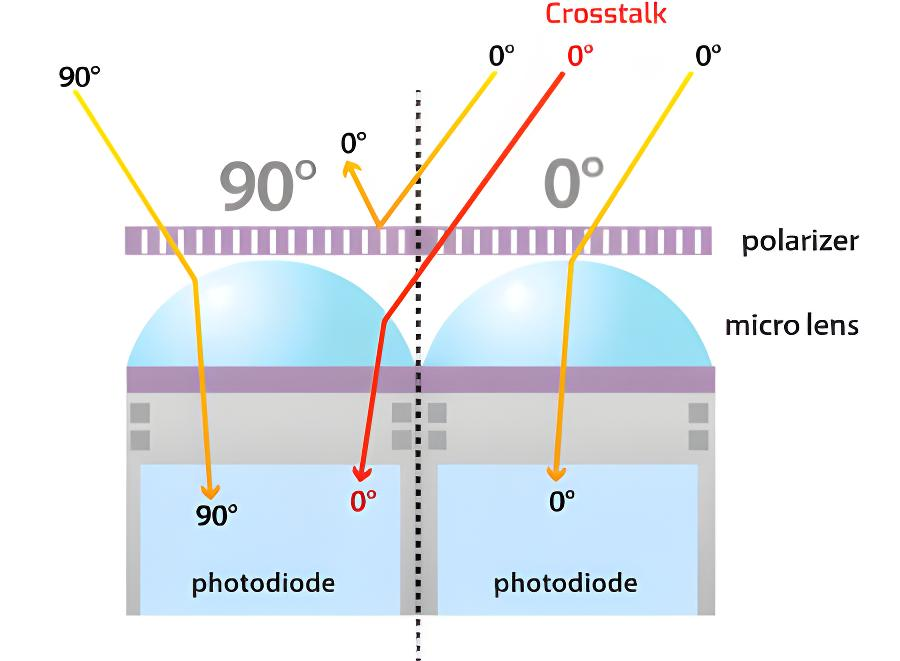
\includegraphics[width=0.8\textwidth]{figures/crosstalk_upscaled.jpg}
    \caption{$0^{\circ}$ polarized light is entering the pixel meant to detect $90^{\circ}$ and will be incorrectly detected as $90^{\circ}$.  This crosstalk error happens because the polarization array is placed above the micro lens \cite{lucidvisionlabsPolarizationExplainedSony2018}}
    \label{fig:camera_crosstalk}
\end{figure}



\section{Polarization}

\begin{figure}
    \centering
    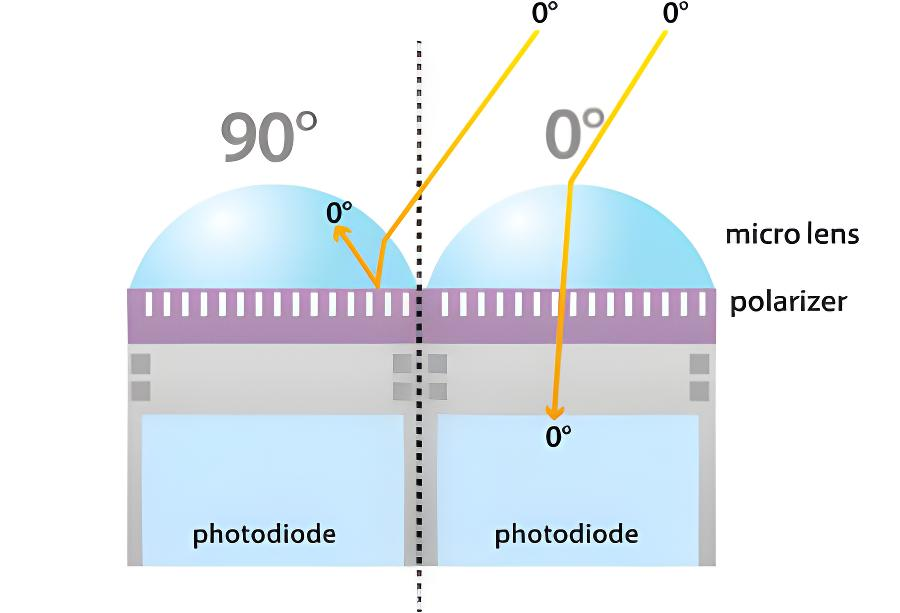
\includegraphics[width=0.8\textwidth]{figures/crosstalk_off_upscaled.jpg}
    \caption{Sony's polarization sensor reduces the chance of crosstalk thanks to the polarizer array being placed on-chip. The $0^{\circ}$ polarized light is unable to enter the pixel meant to detect only $90^{\circ}$ \cite{lucidvisionlabsPolarizationExplainedSony2018}}
    \label{fig:camera_no_crosstalk}
\end{figure}

\begin{figure}
    \centering
    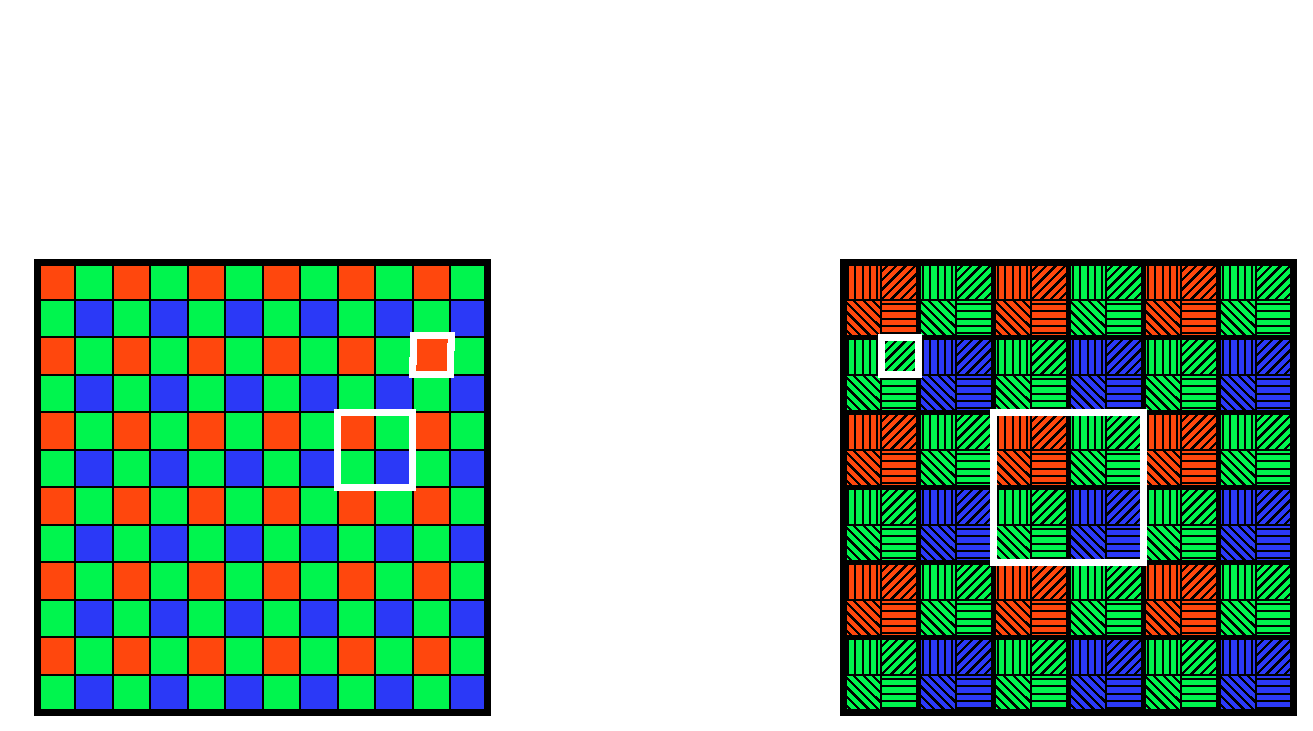
\includegraphics[width=0.8\textwidth]{figures/polarized_image/naming.pdf}
    \caption{Naming convention for the different polarization angles.}
    \label{fig:polarization_naming}
\end{figure}


\section{Configuration}

\section{Nodes}
device 418
interface 23
device 25
system 37

\subsection{10 bit packed}

\subsection{Bugs in the firmware}
Trigger mode stuff.
\section{Synchronization (PPT+PPS)}
Fast mode \approx $50\mu s$. Accurate mode prohibits $20hz$ refresh rate.
Verified using oscilloscope and analog output.
Cameras report ptp offset, but without a proper oscilloscope it is hard to verify if this is correct.

\subsection{Low trigger latency}
It is possible to reduce the trigger latency of the cameras, which results in a lower synchronization offset.
This can be acheived by setting the \code{TriggerLatency} node to \code{OneLine}.
This reduces the average trigger offset down to $10\mu s$.
Unfortunately, this option becomes unavailable while the \code{TriggerOverlap} node is set to \code{set_PreviousFrame}, which is requiered for the cameras to


\subsection{Validation}
\begin{table}[H]
    \centering
    \begin{tabular}{c}
        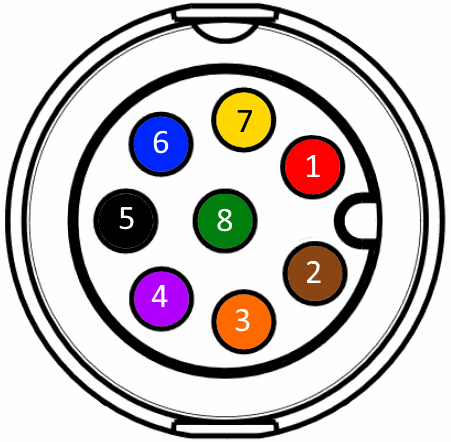
\includegraphics[width=0.3\textwidth]{figures/m8-pin-layout.png}
        \\
        \small
        \begin{tabular}{ |l|l| }
            \hline
            \textbf{Pin} & \textbf{Pin Description}                          \\
            \hline
            1 (Red)      & $V_{AUX}$ (12-24V DC Power Input)                 \\
            2 (Brown)    & Non-isolated bi-directional GPIO channel (Line 2) \\
            3 (Orange)   & VDD GPIO (2.5V Power Output) (Line 4)             \\
            4 (Purple)   & Non-isolated bi-directional GPIO channel (Line 3) \\
            5 (Black)    & GND (Camera GND)                                  \\
            6 (Blue)     & OPTO GND (Opto-isolated Reference)                \\
            7 (Yellow)   & OPTO OUT (Opto-isolated Output) (Line 1)          \\
            8 (Green)    & OPTO IN (Opto-isolated Input) (Line 0)            \\
            \hline
        \end{tabular}
    \end{tabular}
    \caption{\cam \gls{gpio} connector \cite{lucidvisionlabsTritonMPPolarized2020}}

\end{table}


\begin{figure}[H]
    \centering
    \subcaptionbox{Synchronization at $25ms$ resolution}{
        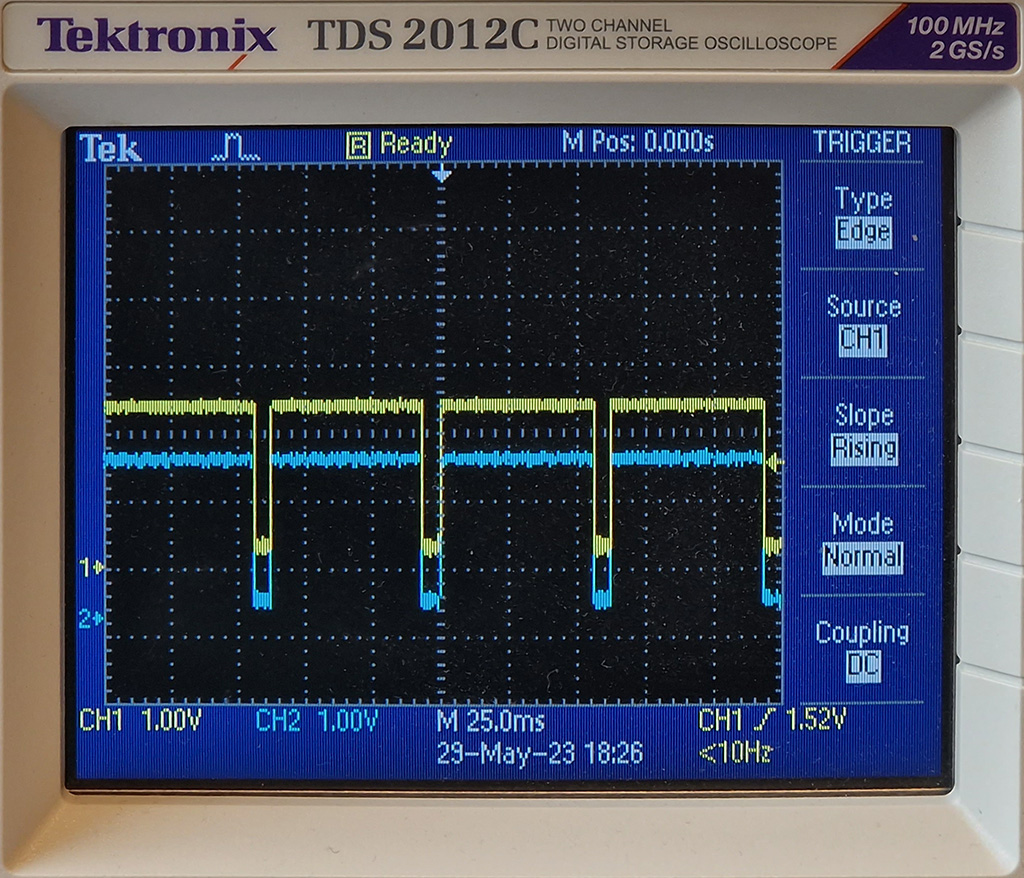
\includegraphics[width=0.8\textwidth]{figures/synchronization/ms.jpg}
    }
    \subcaptionbox{Synchronization at $10\mu s$ resolution}{
        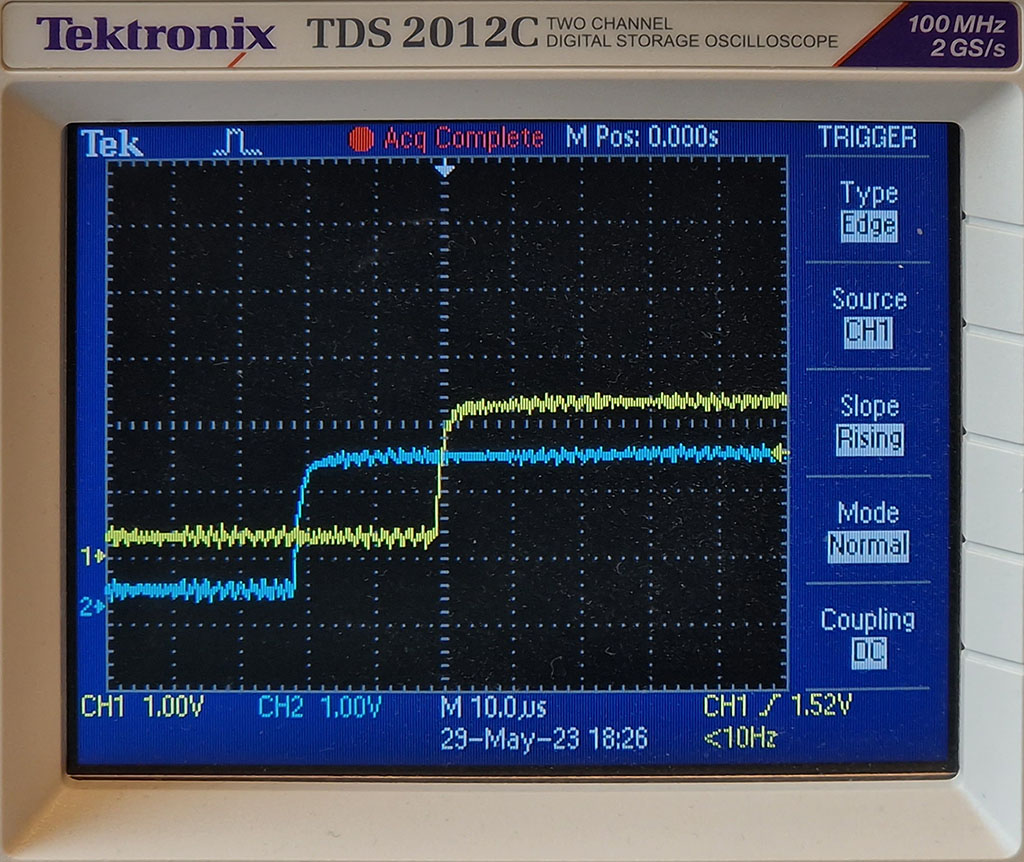
\includegraphics[width=0.8\textwidth]{figures/synchronization/us.jpg}
    }
    \caption{Measured synchronization offset of $22\mu s$ between the two cameras.}
\end{figure}

% \begin{align}
%     \frac{50\mu s}
% \end{align}
\section{Network configuration}
The \jx has a built in etherned adapter and the one osed on the \sr has been equipped with an extra WiFi adapter, as well as a network card consisting of four independant ethernet adapters \cite{martensPortableSensorRig2022}.
The following section describes the different network configurations necessary to connect and communicate with the cameras.
First two essential concepts are explained, then a IP configuration setup used to automatically detect the cammeras and assign IP adresses is presented.


\subsubsection{Reverse Path Filtering}
\gls{rpf} is a security feature that is designed to prevent IP address spoofing attacks by discarding incoming network traffic that does not have a valid return path \cite{ReversePathFiltering}.
However, in some cases, such as when discovering cameras over \gls{gigev} using \gls{lla}, disabling \gls{rpf} may be necessary ensure detection \cite{lucidvisionlabsArenaSoftwareDevelopment2020}.
This can for example occur if the cameras IP address collides with that of the network adapter \cite{lucidvisionlabsArenaSoftwareDevelopment2020}.
The followinc command can be used to disable \gls{rpf} \code{sudo sysctl -w net.ipv4.conf.eth1.rp_filter=0}.

\subsubsection{Link-Local Adress}
% In computer networking, \gls{lla} refers to an IP address that is used for communication within a logical division or broadcast domain to which the host is connected \cite{annieahujaweb2020LinkLocalAddress2022}.
% \gls{lla} is unique within a network segment, but not across different network segments, and therefore should not be forwarded by routers, this is however not relevant for this application \cite{annieahujaweb2020LinkLocalAddress2022}.
\gls{lla} is a method of IP address assignment that is often used when working with \gls{gigev} cameras \cite{teledyneSettingIPAddress01} \cite{lucidvisionlabsArenaSoftwareDevelopment2020}.
It allows devices to automatically assign IP addresses without the need for a \gls{dhcp} server or static IP \cite{annieahujaweb2020LinkLocalAddress2022}, which makes it possible to connect a \gls{gigev} camera directly to an ethernet adapter, without the need for an intermediate router.
For this to work properly the network adapter shoud be assigned the IP \code{169.254.0.1} and have netmask \code{255.255.0.0} as \gls{lla} addresses are assigned within the scope of \code{169.254.1.0} to \code{169.254.254.255} \cite{annieahujaweb2020LinkLocalAddress2022}\cite{lucidvisionlabsArenaSoftwareDevelopment2020}.

\subsubsection{Static IP}
A static IP address is one that is set up manually on a device, rather than being allocated by a DHCP server.
It is referred to as static since it remains constant, in contrast to a dynamic IP address that can vary.
\cite{fisherStaticIPAddresses2021}.
For \gls{gigev} Cameras using statid IP might be usefull as the cameras will power up with the same IP every time \cite{teledyneSettingPersistentIP}.

However I decided not to use static IP for the sensor rig setup, as it requiered the camera to be connected to the same ethernet port every time.
If the static IP of a camera was outside the IP range (\todo) of the network adapter it was connected to, or the network adapters had ovelapping IP ranges, the discovery process and connection got unstable.
Thus, to change which ethernet port a camera was connected to it would be necessary to either change the static IP of the camera, a tedious process, or change the IP range of both the current and previous ethernet adaptor.
An additional rationale for avoiding the use of static IP addresses is to keep the cameras' static configurations (the ones that persists when power cycling) the same as facory default.
This facilitates the use of the same cameras for a different project by someone else in the future.

\subsubsection{IP configuration pipeline}
The IP configuration pipeline is adapted to the discovery and enumeration process of the \lucid cameras, which is outlined in Figure \ref{fig:lucid_ip_discovery}.
The main idea is that as persistant IP is not enabled and there is no DHCP client on the \jx, each camera will initialy use \gls{lla}.



\subsection{Network Performance}
As each camera produces close to $1Gb$ of data per second, several network configurations have to be done in order for the \jx to handle all the incoming traffic.

\subsubsection{Jumbo Frames}
An Ethernet frame is a unit of packetized formatted information that includes the Ethernet header, payload, and CRC trailer.
\cite{winterCisco3ComApplied2009}.
The original Ethernet specification, IEEE 802.3 \cite{ieeeIEEEStandardsInterpretation2002}, allowed for a frame size between 64 to 1518 bytes, with a standard header length of 18 bytes.
Ethernet Jumbo frames carry more payload than the maximum specified by IEEE 802.3, with an \gls{mtu} size of up to 9000 bytes \cite{lucidvisionlabsJumboFramesLUCID2020}.
Increasing the maximal \gls{mtu} size typically leads to improved performance for high-bandwidth cameras and can also help reduce the CPU load on the host system \cite{lucidvisionlabsJumboFramesLUCID2020}, as there is less protocol overhead \cite{lukeThingsYouShould2018}.
Both the ethernet card used on the \jx as well as the \cams support Jumbo frames \cite{IntelI350am4Chip} \cite{lucidvisionlabsTritonMPPolarized2020}.
To enable jumbo frames on a device (\code{eth1}) the following command is used \code{ifconfig eth1 mtu 9000}.

\subsubsection{Receive Buffers}
\begin{figure}
    \centering
    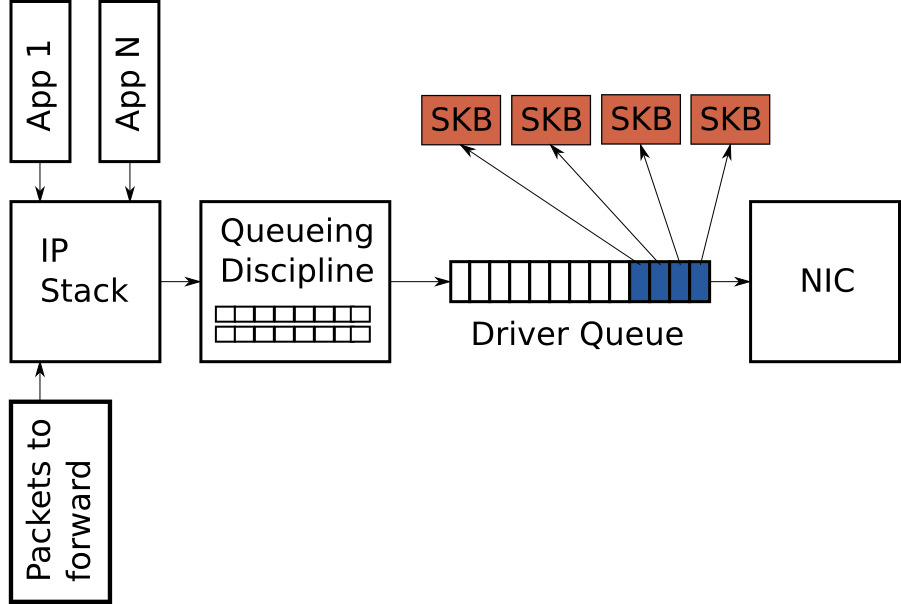
\includegraphics[width=0.8\textwidth]{figures/linux_networking.png}
    \caption{Simplified high level overview of the queues on the transmit path of the Linux network stack \cite{danQueueingLinuxNetwork2013}}
    \label{fig:linux_network}
\end{figure}
When network packets arrive on Linux they are stored in a driver queue as shown in Figure \ref{fig:linux_network} \cite{danQueueingLinuxNetwork2013}.
To avoid starvation and increase performance, it is recommended to increase the default number of \glspl{skb}, also known as receive buffers \cite{lucidvisionlabsReceiveBuffers2020} \cite{danQueueingLinuxNetwork2013}.
This can be done using the \mintinline{bash}{ethtool -G} command \cite{danQueueingLinuxNetwork2013}.
The maximal allowed number of receive buffers on the \jx are 4096, opposed to the default value of 256, according to the \mintinline{bash}{ethtool -g eth1} command.
The poetntial downside of increasing the number of \glspl{skb} is that it increases the memory usage and it might introduce more Latency as the Driver Queue gets longer \cite{danQueueingLinuxNetwork2013}.
As the current use case for the sensor platform is to record data, this is not a problem, but it should be kept in mind for future work if the sensor platform is used for real-time applications.

As we are receiving large amounts of data as jumbo frames it is also recommended to increase the default and the maximal socket buffer size.
The default values for the default and maximal receive buffer saize were \todo and \todo, which was found using the \mintinline{bash}{sysctl -a | grep rmem_default} and \mintinline{bash}{sysctl -a | grep rmem_max} commands on a newly booted \jx \cite{sainiUnableReadNet2021}.

\lucid suggests setting both default and max buffer size to $1MiB$ while IBM suggest setting them up to $16MB$ for best performance \cite{lucidvisionlabsReceiveBuffers2020}\cite{ibmIBMDocumentationTCPIP2021}.
As it is quite cumbersome to perform low level network latency analysis, and memory depletion never seemed to be an issue with the $16GB$ of \gls{ram} available on the \jx, both default and max buffer size was set to $16MiB$.
To make this change permanent the following command is used \cite{redhat10ChangingNetwork}.
\begin{minted}{bash}
    $ sudo sh -c "echo 'net.core.rmem_default=16777216' >> /etc/sysctl.conf"
    $ sudo sh -c "echo 'net.core.rmem_max=16777216' >> /etc/sysctl.conf"
    $ sudo sysctl -p
\end{minted}

\begin{figure}
    \centering
    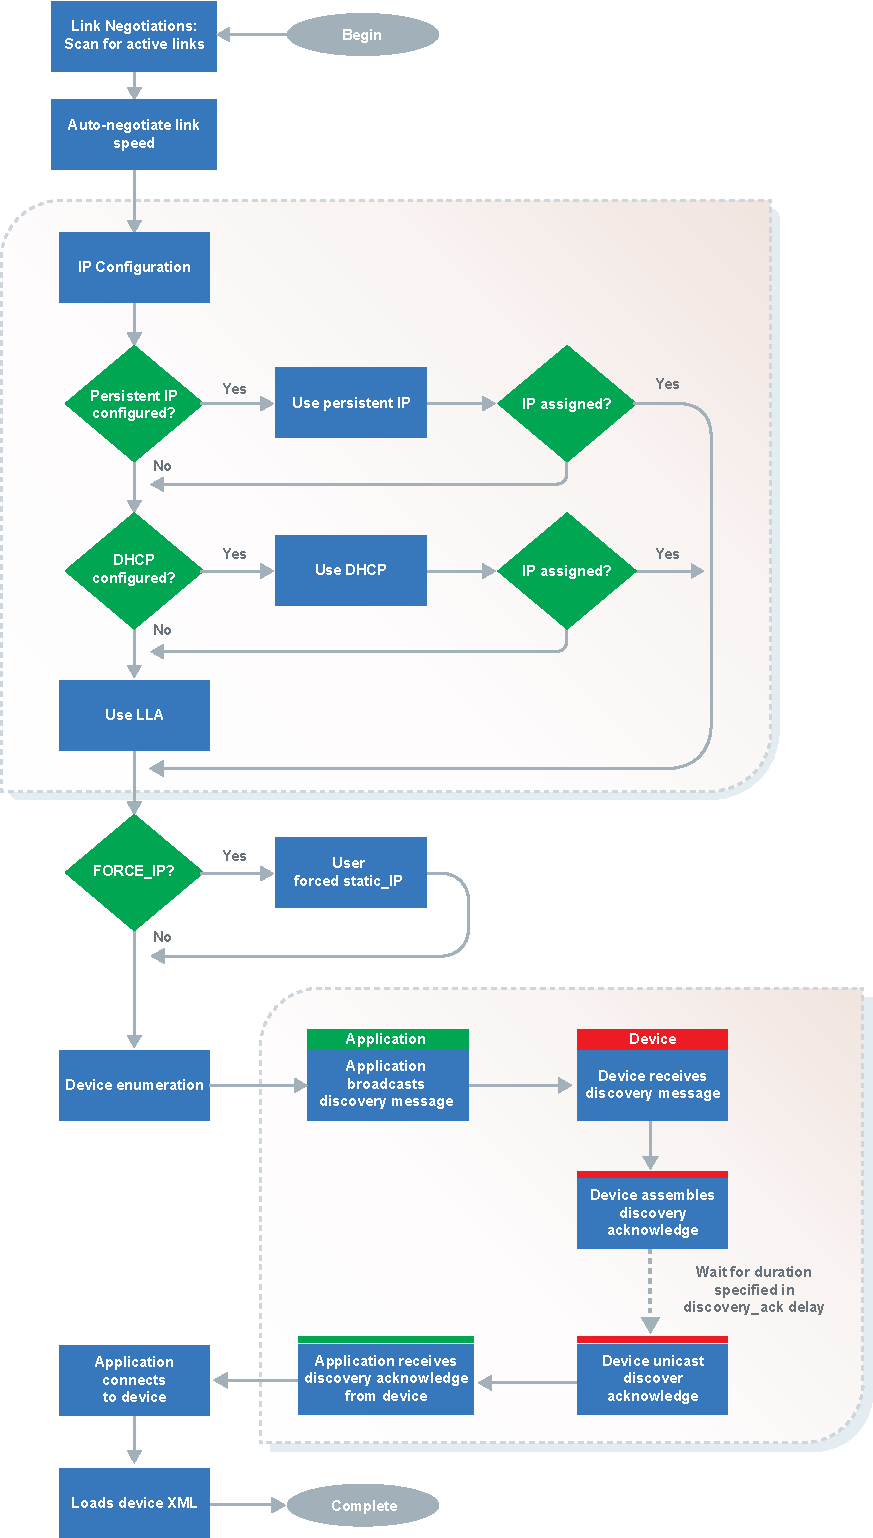
\includegraphics[height=\textheight]{figures/PDF/lucid_ip_discovery.pdf}
    \caption{Figure of the descovery and enumeration process of Lucid cameras \cite{lucidvisionlabsTritonMPPolarized2020}}
    \label{fig:lucid_ip_discovery}
\end{figure}
\chapter{Programming Theory}
\section{Concurrent programming}
Concurrency is an essential concept in computer science that enables multiple tasks to run simultaneously in a program.
This section introduces the concept of concurrent programming and discusses the different concepts associated with it.


\subsection{Sequential programming}
To understand concurrent programming, we must first understand sequential programming.
Sequential programming is a programming paradigm in which one task is finished before the next one is started.
This can be seen as the default type of programming where one line of code is executed after another in a linear order.
Figure \ref{fig:concurrency_sequential} shows an example of sequential program that executes a sequence of three tasks multiple times.

\begin{figure}[H]
    \centering
    
\includegraphics[width=\textwidth]{figures/concurrency/sequential.pdf}
    \caption{Sequential programming}
    \label{fig:concurrency_sequential}
\end{figure}

If there is no reason to execute tasks concurrently, then sequential programming is often the best choice as there is little to no overhead involved and it is easy to understand, debug and maintain.

\subsection{Concurrent programming}
Concurrent programming is a programming paradigm in which multiple tasks are executed simultaneously, instead of in a sequential manner.


Concurrent programming can be split into two categories, asynchronous and parallel.


\subsection{Asynchronous programming}
Asynchronous programming is a programming paradigm in which tasks are executed concurrently without blocking the execution of other tasks.
In an asynchronous program, tasks are typically executed in a non-blocking manner, allowing the program to continue executing while waiting for the results of a particular task.

\begin{figure}[H]
    \centering
    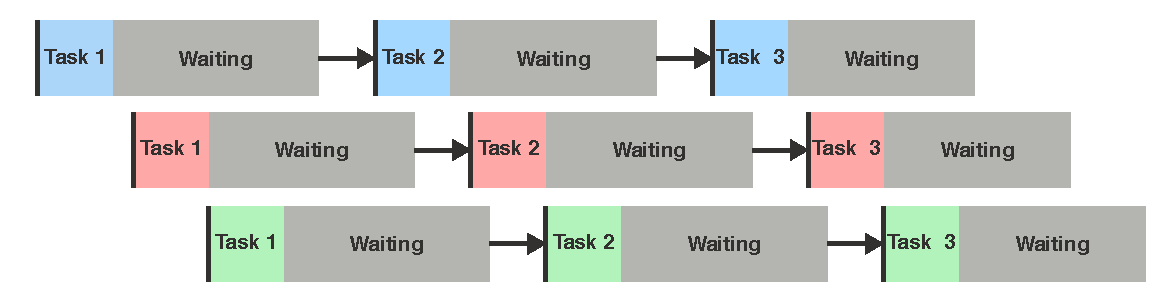
\includegraphics[width=\textwidth]{figures/concurrency/concurrent.pdf}
    \caption{Asynchronous programming}
    \label{fig:concurrency_concurrent}
\end{figure}

Asynchronous programming is often used in systems that perform I/O operations, such as network communication or file I/O, where waiting for the results of an operation can be time-consuming.
Rather than blocking the program until the operation is complete, an asynchronous program can execute other tasks while waiting for the operation to complete.

Asynchronous programming can be achieved through various techniques, including callbacks, promises, and async/await syntax.
With callbacks, a function is called when an asynchronous operation is completed, while promises provide a more structured way of handling asynchronous operations by allowing for the chaining of multiple operations.
The async/await syntax provides a more concise way of writing asynchronous code by using keywords to indicate that a function is asynchronous and that it is awaiting the completion of a particular operation.

Asynchronous programming is becoming increasingly important in modern software development, as it can improve the performance and scalability of applications, particularly in systems that involve large amounts of I/O operations.
However, it can be challenging to write and debug asynchronous code, as developers must be careful to avoid race conditions and other synchronization issues.

\subsection{Parallel programming}


Parallel programming is a programming paradigm in which multiple tasks or parts of a program are executed simultaneously on multiple processors or cores, with the goal of improving the performance and efficiency of the program.
In a parallel program, tasks can be divided into smaller sub-tasks that can be executed concurrently, potentially reducing the overall time required to complete the task.

\begin{figure}[H]
    \centering
    
\includegraphics[width=\textwidth]{figures/concurrency/paralell.pdf}
    \caption{Parallel programming}
    \label{fig:concurrency_parallel}
\end{figure}

Parallel programming can be achieved through various techniques, including multithreading, multiprocessing, and distributed computing.
Multithreading involves running multiple threads of execution within a single process, while multiprocessing involves running multiple processes in parallel.
Distributed computing involves running parts of a program on multiple machines connected through a network.

Parallel programming can provide significant performance benefits in systems that are designed to take advantage of multiple processors or cores.
However, designing parallel programs can be challenging, as developers must carefully manage resources and avoid synchronization issues, such as race conditions and deadlocks.

Parallel programming is becoming increasingly important in modern software development, as the number of cores and processors in computers and other devices continues to increase, and as more applications are designed to take advantage of parallel processing.
It is particularly important in areas such as scientific computing, data analysis, and artificial intelligence, where large amounts of data must be processed in a timely manner.


\subsection{Design patterns}
\todo
\begin{itemize}
    \item Can the task be done in parallel?
    \item Does the task require a lot of memory?
    \item Does the order of output matter?
    \item Is latency an issue?
    \item Is there any bottlenecks?
    \item What tasks are resource intensive?
\end{itemize}
\begin{figure}[H]
    \centering
    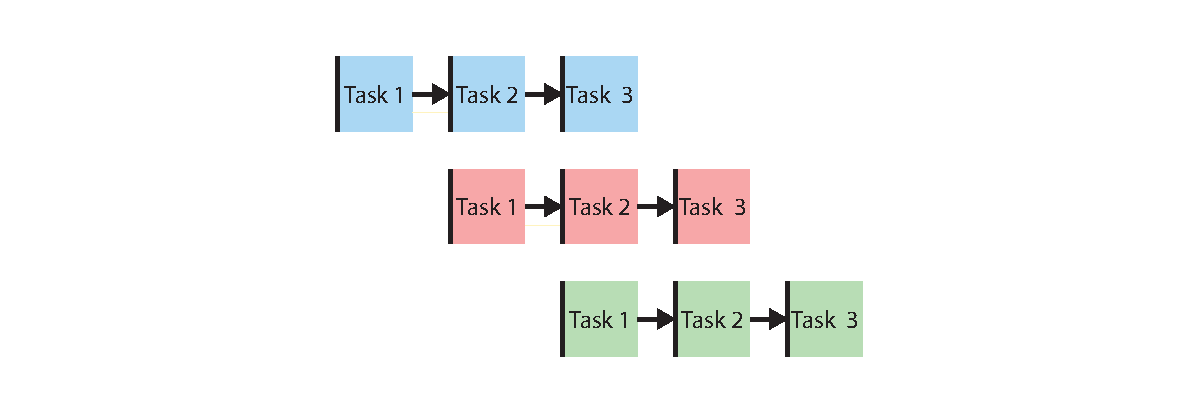
\includegraphics[width=\textwidth]{figures/concurrency/concurrent_overlap.pdf}
    \caption{Parallel programming}
    \label{fig:concurrency_concurrent_overlap}
\end{figure}

\begin{figure}[H]
    \centering
    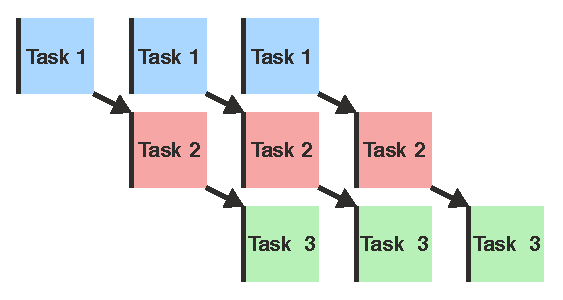
\includegraphics[width=\textwidth]{figures/concurrency/thread_per_task.pdf}
    \caption{Parallel programming}
    \label{fig:concurrency_thread_per_task}
\end{figure}


\begin{figure}[H]
    \centering
    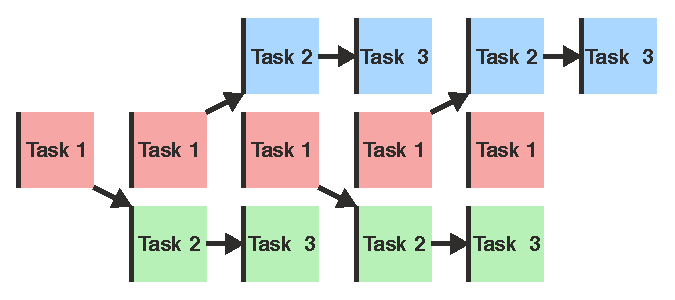
\includegraphics[width=\textwidth]{figures/concurrency/distribute.pdf}
    \caption{Parallel programming}
    \label{fig:concurrency_distribute}
\end{figure}


\section{GPU programming in CUDA}
In recent years, there has been a significant shift towards parallel computing in order to achieve faster processing times and better performance.
The rise of \glspl{gpu} has been a major factor in enabling parallel computing for a wide range of applications, from machine learning to scientific simulations.
One of the most popular platforms for parallel computing on GPUs is \gls{cuda} developed by NVIDIA, which is a framework and programming model for parallel computing on NVIDIA \glspl{gpu}.

CUDA is a parallel computing platform and programming model developed by NVIDIA that allows developers to harness the power of their GPUs for a wide range of applications.

Programming for GPUs is fundamentally different from programming for CPUs.
While CPUs have a small number of powerful cores, GPUs have a much larger number of simpler cores.
This means that code needs to be structured differently to take advantage of the parallelism offered by GPUs.
In addition, data transfer between the CPU and GPU can be a bottleneck, so care must be taken to optimize data movement.

In this chapter, we will explore the basics of CUDA programming, including the key differences between programming for CPUs and GPUs, and the general workflow of programming in CUDA.
We will cover topics such as device memory management, kernel functions, and thread synchronization.


\subsection{Heterogeneous Computing}
Heterogeneous computing refers to a programming model where multiple different types of computing cores cooporate to solve groups of tasks in an efficient manner \cite{armWhatHeterogenousCompute}.
The \jx is a good example of this; equiped with an 8-core ARM \gls{cpu} and a 512-core NVIDIA \gls{gpu}, as well as several \glspl{asic} including an \gls{isp}, \gls{dla} and two \glspl{nvenc} for specific media encoding and decoding \cite[9, 8, 23, 15-22]{nvidiaNVIDIAJetsonAGX2019}.
This combination of different types of cores working together allows for a system to efficiently handle a wide range of tasks, from general-purpose computing to specialized tasks such as video processing and compression.

\begin{figure}
    \centering
    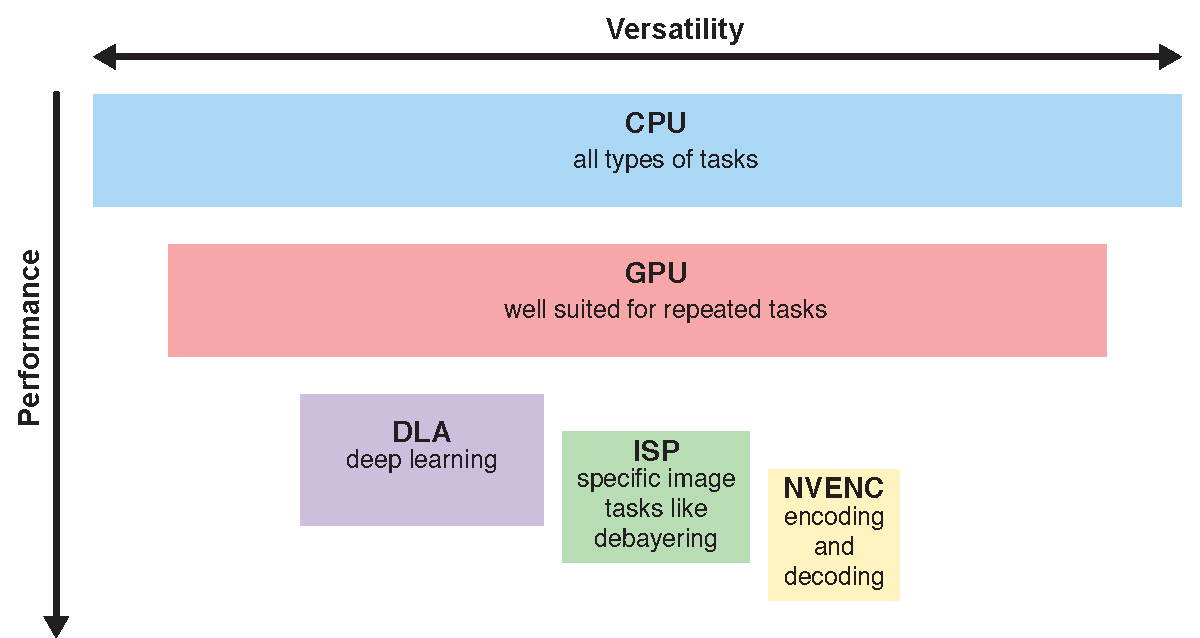
\includegraphics[width=\textwidth]{figures/PDF/jx_hierarchy.pdf}
    \caption{Illustration of the versatility and performance of different types of cores on the \jx.}
    \label{fig:jx_hierarchy}
\end{figure}


\subsubsection{Memory Management}
With different types of cores comes different types of memory.
A key challenge of working with heterogeneous computing systems is to manage the different types of memory efficiently, so that the different cores have access to the data they need when they need it.

A major advantage of working on the \jx is the posibility to share memory between the different types of cores, removing the need for expensive data transfers between the different types of memory.
This is further discussed in Section \ref{sec:jx_memory}.

\begin{figure}
    \centering
    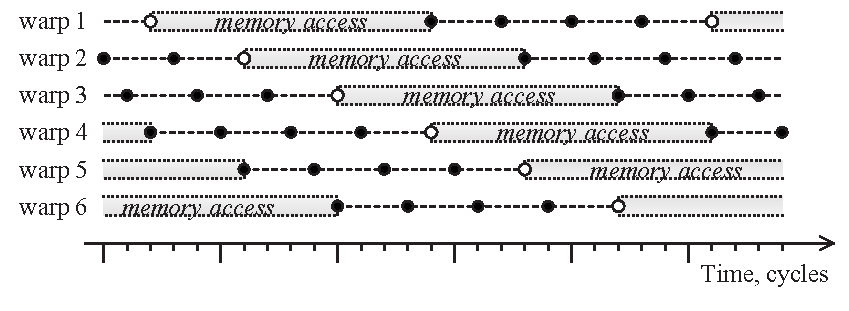
\includegraphics[width=\textwidth]{figures/PDF/concurrency_p54.pdf}
    \caption{Visualization of concurrent execution on a GPU \cite[54]{volkovLatencyHiding2016}}
    \label{fig:concurrency}
\end{figure}


\subsubsection{Latency Hiding}
Latency hiding is a technique used by modern commodity processors such as GPUs to better utilize their numerous execution units and hide execution latencies \cite[35]{volkovLatencyHiding2016}
The idea behind latency hiding is to keep the processor busy with other tasks while it waits for data to be fetched from memory.
This is achieved by executing multiple threads in parallel, so that when one thread is waiting for data, another thread can continue executing.


\subsubsection{Profiling}
Profiling is the process of measuring the performance of a program, and is an important tool for optimizing programs.

In many cases it is straight forward; record the time when a task is started and when it is finished, and calculate the difference.


However, when working with heterogeneous computing systems, it is not always

nsys memory profiling does not work in Pinned Memory



\section{Debugging and Profiling}

\subsection{Throughput and Latency}
In sequential programming measuring the performance of a program can be done through measuring its execution time.
This can be acheived by recording the time when the program starts and when it finishes, and calculating the difference.
The througput then becomes the

The impact of future optimizations can then be measured by comparing the execution times before and after the optimizations are applied.
As the number of tasks that can be solved in a given time is

However, in concurrent processing, execution times of individual instructions may overlap, making it challenging to calculate the execution time of the individual instructions \cite[21]{volkovLatencyHiding2016}.
The same type for time measurements can still be performed, but i

Instead, metrics such as latency, throughput, and concurrency can be used to characterize the process.

For example, latency is the average time between the start and end times of individual items, while throughput is the number of items processed within a given time interval divided by the duration of the interval.
Concurrency is the number of items processed simultaneously and can be measured at different moments in time or as an average over a particular interval.

\subsection{MVP}

\begin{listing}[H]
    \begin{minted}{python}
        def sleep_1sec(): time.sleep(1)
        async def sleep_1sec_async(): await asyncio.sleep(1)

        async def test_asyncio():
            await asyncio.gather(*[sleep_1sec_async() for _ in range(N)])

        def test_thread_pool():
            with ThreadPoolExecutor(max_workers=10000) as ex:
                futures = [ex.submit(sleep_1sec) for _ in range(N)]

        async def test_thread_pool_async():
            loop = asyncio.get_event_loop()
            with ThreadPoolExecutor(max_workers=10000) as ex:
                asyncio.gather(*[loop.run_in_executor(ex, sleep_1sec) for _ in range(10000)])

        def test_threads():
            threads = [threading.Thread(target=do_nothing) for _ in range(10000)]
            [thread.start() for thread in threads]
            [thread.join() for thread in threads]
    \end{minted}
    \caption{Code used to compatre asyncio and threads.}
    \label{listing:concurrency_test}
\end{listing}
\begin{listing}[H]
    \begin{minted}{bash}
        >>> test_asyncio took 1.373797 seconds to complete.
        >>> test_thread_pool took 4.091199 seconds to complete.
        >>> test_thread_pool_async took 4.391777 seconds to complete.
        >>> test_threads took 5.373108 seconds to complete.
    \end{minted}
    \caption{Results when running the code in Listing  \ref{listing:concurrency_test} on the \jx}
\end{listing}


% \begin{listing}[H]
%     \begin{minted}{python}
%         import asyncio, threading, time

%         def do_nothing(): pass
%         async def do_nothing_async(): pass

%         async def test_asyncio():
%             start_time = time.perf_counter()
%             await asyncio.gather(*[do_nothing_async() for _ in range(10000)])
%             end_time = time.perf_counter()
%             print(f"Asyncio took {end_time - start_time:.6f} seconds to complete.")

%         def test_threads():
%             threads = [threading.Thread(target=do_nothing) for _ in range(10000)]
%             start_time = time.perf_counter()
%             for thread in threads:
%                 thread.start()
%             for thread in threads:
%                 thread.join()
%             end_time = time.perf_counter()
%             print(f"Threads took {end_time - start_time:.6f} seconds to complete.")

%         if __name__ == "__main__":
%             asyncio.run(test_asyncio())
%             test_threads()
%     \end{minted}
%     \begin{minted}{bash}
%         >>> Asyncio took 0.311703 seconds to complete.
%         >>> Threads took 11.898036 seconds to complete.
%     \end{minted}
%     \caption{Comparison of asyncio and threads running on INTEL i7-11800H @ 2.30GHz.}
% \end{listing}
\section{Memory management on Jetson platform}
\label{sec:jx_memory}
On \gls{tegra} platforms, there are different types of memory available for use, including device memory, pageable host memory, pinned memory, and unified memory docs.nvidia.com.
These memory types are allocated on the same physical SoC DRAM but have different accessing and caching behaviors.
Device memory is used for buffers limited to \gls{igpu} access, pageable host memory is used for buffers limited to CPU access, pinned memory is recommended for small buffers, and unified memory is cached on both \gls{igpu} and CPU \cite{nvidiaCUDAFTegra2023}.


\subsection{Memory types}
This section presents the different memoty types available on the \jx.
It builds upon the CUDA for Tegra documentation \cite{nvidiaCUDAFTegra2023}, with a focus on what is relevant for the setup on the \sr, where ther is a \jx with compute cabability of 7.2 \cite{CUDA2023} and no external \gls{dgpu}.
A summary of the different memory types is presented in Table \ref{tab:memory_types}.


\providecommand{\tmpfootnote}{\footnote{Cached where compute capability is greater than or equal to 7.2 \cite
        {nvidiaCUDAFTegra2023}. The \jx has compute capability of 7.2 \cite{CUDA2023} }}
\begin{table}
    \centering
    \begin{tabular}{ |c|c|c| }
        \hline
        \textbf{Memory Type} & \textbf{CPU}            & \textbf{iGPU}           \\
        \hline
        Pageable host memory & Cached                  & Not directly accessible \\
        Device memory        & Not directly accessible & Cached                  \\
        Pinned host memory   & Cached                  & Uncached                \\
        Pageable host memory & Cached                  & Cached                  \\
        \hline
    \end{tabular}
    \caption{Memory types on the \jx \cite{nvidiaCUDAFTegra2023}}
    \label{tab:memory_types}
\end{table}
\subsubsection{Pageable host memory}
Pageable host memory, is the normal type of memory used on the \jx,
e.g. it is what is used allocated with \code{malloc} and used to store normal \py objects.
When memory is pageable the \cpu can control where it is stored, and it can be moved to the \gls{swap} area to free up physical memory \cite[6]{nvidiaCUDAFTegra2023}.
This is why it is not directly accessible by the \gls{igpu}.
If memory is not accesed by the \gls{igpu}, pageable memory should be used \cite[9]{nvidiaCUDAFTegra2023}


\subsubsection{Device memory}
Device memory is memory that is directly accessible by the \gls{igpu} but not the \cpu \cite[5]{nvidiaCUDAFTegra2023}.
It is allocated on the same physical SoC DRAM as other memory types, but cached in a way that is optimized for \gpu usage, making in unacessable on the \cpu \cite[5]{nvidiaCUDAFTegra2023}.


\subsubsection{Pinned host memory}
Pinned memory, also known as page-locked memory, is a type of memory that is directly accessible by both the CPU and the iGPU in \gls{tegra} systems \cite{nvidiaCUDAFTegra2023}.
Pinned memory reduces data transfer overhead between the CPU and iGPU because it can be directly accessed by both \cite{nvidiaCUDAFTegra2023}.
However, it is worth noting that pinned memory can lead to increased memory usage as it is not pageable, and should therefore not be used everywhere \cite[38]{nvidiaCUDABestPractices2023}.
It is also not cached on the \gls{igpu}, making it less efficient if the same data is accessed multiple times \cite{nvidiaCUDAFTegra2023}.
However as is discussed in Section \todo, the data from the camera is read only once, making the following statement relevant:
\say{For large buffers, when the buffer is accessed only once on iGPU in a coalescing manner, performance on iGPU can be as good as unified memory on iGPU.}\cite[10]{nvidiaCUDAFTegra2023}


\subsubsection{Unified memory}
Unified memory is acessable and cached on both the \gls{igpu} and the \cpu, making it a good choice for memory that is repeadetly acessed from both devices \cite[10]{nvidiaCUDAFTegra2023}.
The downside of unified memory, compared to pinned memory is that the overhead from cache maintenance operations \cite[12]{nvidiaCUDAFTegra2023}.
The performance can be improved by manually prefetching data, at the cost of making the code more complex \cite[13]{nvidiaCUDAFTegra2023}.
Unified memory was tested on the \sr, but the performance was worse, compared to pinned memory and using pinned memory resulted in fewer lines and more readable code.


\subsubsection{NVMM memory}

\chapter{Efficient Preprocessing of Raw Image Data in CUDA}
\label{chap:debayer}

To compress the video frames from the cameras, it is necessary to first transform the data into a format that is compatible with the encoder.
This involves debayering the data to extract color information, converting the extracted color into a different color space, and packaging the data in a specific format.
Since the cameras utilize a specialized image sensor, a custom preprocessor was developed to perform these operations.
The preprocessor takes the raw bytes from the cameras as input and generates bytes that can be directly sent to the H.265 encoder.
In order to achieve the required throughput and limit power consumption, the preprocessor is implemented using\gls{cuda}.

This chapter provides an overview of the theory behind debayering and color spaces, and presents the optimized\gls{cuda} implementation.


\subsection{Bayer filter}
To capture color images conventional cameras use \glspl{cfa}.
The most common type of \gls{cfa} is the Bayer pattern where green pixels cover half the array in a lattice, and the red and blue pixel locations are spaced between the green pixels as shown in Figure \ref{fig:bayer_pattern} \cite{getreuerMalvarHeCutlerLinearImage2011}.
Different orderings of the colors in the \gls{cfa} exists, with the most common ones being RGGB, BGGR, GRBG, and GBRG where the letters designate the order of the four top left pixeld in the image.

\begin{figure}[H]
    \centering
    \begin{tabular}[b]{ccc}
        \subcaptionbox{RGGB bayer pattern}{
\includegraphics[width=0.25\textwidth]{figures/debayer/bayer_pattern.pdf}
            \label{fig:bayer_pattern}
        }                                                                                                              &
        \subcaptionbox{Green at red}{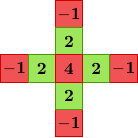
\includegraphics[width=0.25\linewidth]{figures/debayer/g_at_r.png}}               &
        \subcaptionbox{Green at red}{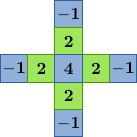
\includegraphics[width=0.25\textwidth]{figures/debayer/g_at_b.png}}                 \\
        \subcaptionbox{Red at }{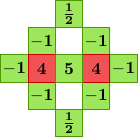
\includegraphics[width=0.25\textwidth]{figures/debayer/r_at_g_rr.png}}                 &
        \subcaptionbox{Red at green, blue row}{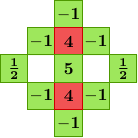
\includegraphics[width=0.25\textwidth]{figures/debayer/r_at_g_br.png}}  &
        \subcaptionbox{Red at blue}{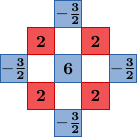
\includegraphics[width=0.25\textwidth]{figures/debayer/r_at_b.png}}                  \\
        \subcaptionbox{Blue at green, red row}{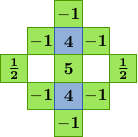
\includegraphics[width=0.25\textwidth]{figures/debayer/b_at_g_rr.png}}  &
        \subcaptionbox{Blue at green, blue row}{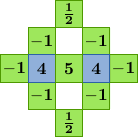
\includegraphics[width=0.25\textwidth]{figures/debayer/b_at_g_br.png}} &
        \subcaptionbox{Blue at red}{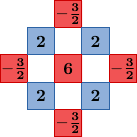
\includegraphics[width=0.25\textwidth]{figures/debayer/b_at_r.png}}
    \end{tabular}
    \caption{Bayer pattern and coefficient values used by Malvar-He-Cutler scaled by 8 \cite{getreuerMalvarHeCutlerLinearImage2011}\cite{CommonsBayerPattern2020}}
    \label{fig:debayer:malvar_filters}
\end{figure}

\subsection{Image demosaicing}
Image demosaicing is the process of estimating full-resolution color information for an image that has been captured with a bayer pattern \cite{liImageDemosaicingSystematic2008}, e.g. at each red pixel in the \gls{cfa} the green and blue intensities needs to be estimated.
Simple methods, such nearest neighbours or linear interpolation, are prone to yielding images false colors and the checkboard like patterns called the zipper effect as shown in Figure \ref{fig:artifacts_gioia} \cite{gioiaDataDrivenConvolutionalModel2021} \cite{liImageDemosaicingSystematic2008}.
A multitude of more advanced methods have been proposed with increasing sofisication and performance \cite{liImageDemosaicingSystematic2008}.
Lately different deep learning methods has also proven to perform very well at this task \cite{kwanComparisonDeepLearning2019}.

\begin{figure}[H]
    \centering
    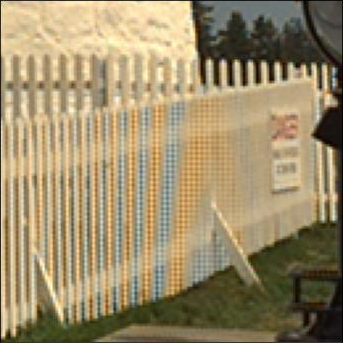
\includegraphics[width=0.5\textwidth]{figures/debayer/artifacts_gioia.png}
    \caption{Zipper effect and false colors \cite{gioiaDataDrivenConvolutionalModel2021}}
    \label{fig:artifacts_gioioa}
\end{figure}

\subsection{Malvar-He-Cutler}
\gls{mhc} pattented a simple but performant linear method using 5x5 filters that shows surprisingly good results \cite{malvarHighqualityGradientcorrectedLinear2009}.
The method they present is derived as a modification of bilinear interpolation, and it involves adding Laplacian cross-channel corrections to improve the quality of the bilinear method \cite{getreuerMalvarHeCutlerLinearImage2011}.
The demosaicking is implemented by convolution with a set of linear filters, and there are eight different filters for interpolating the different color components at different locations as can be shown in Figure \ref{fig:debayer:malvar_filters}.
Although several more sophisticated methods have been developed, the simple \gls{mhc} method works remarkably well \cite{liImageDemosaicingSystematic2008}\cite{kwanComparisonDeepLearning2019}\cite{getreuerMalvarHeCutlerLinearImage2011}.
The method is better suited for parallel execution than some others as discussed in \todo.



\subsection{Shortcomings}
A shortcoming of the current method is that it does not use optimal gains.
Firstly the values used in \gls{mhc} are rounded to the neared dyadic rationals, to work efficently using integer arithmetic and bitshifting \cite{getreuerMalvarHeCutlerLinearImage2011}.
As the current proposed implementation uses floating point arithmetic, this rounding is unecessary.
Another minor issues is that the values in \gls{mhc} were found to be the best fit for the well-known public-domain Kodak image set \cite{malvarHighqualityGradientcorrectedLinear2009}.
This is a set of 24 varied images, shown in Figure \ref{fig:kodak_image_suite}, that might not be the best representation of the images the \sr will capture in maritime environments.
It might be beneficial to recalculate the values based on a more representative dataset and use the floating point values rather than the rounded ones in the future.


\begin{figure}[H]
    \centering
    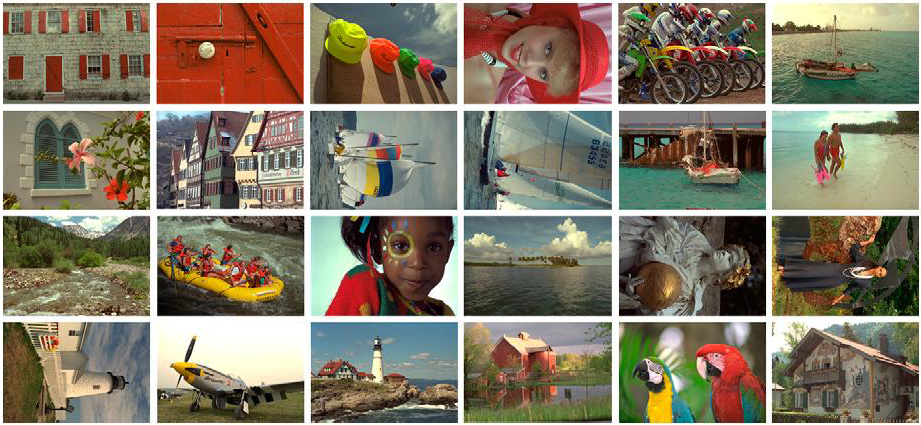
\includegraphics[width=0.8\textwidth]{figures/debayer/kodak_test_suite.png}
    \caption{Kodak image suite \cite{franzenTrueColorKodak2013}\cite{chungAdaptiveColorFilter2006}}
    \label{fig:kodak_image_suite}
\end{figure}


\begin{figure}[H]
    \centering
    \begin{tabular}[b]{ccc}
        \subcaptionbox{Exact image}{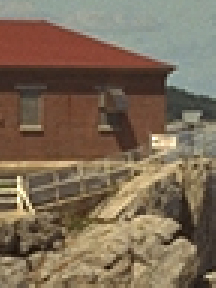
\includegraphics[width=0.3\textwidth]{figures/debayer/house_orig.jpg}}                           &
        \subcaptionbox{Observed Image}{
\includegraphics[width=0.3\textwidth]{figures/debayer/house_bayer.png}}                         \\
        \subcaptionbox{Bilinear (PSNR=25.61)}{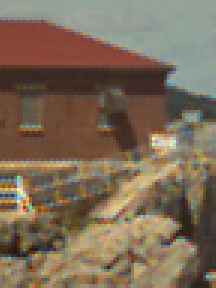
\includegraphics[width=0.3\textwidth]{figures/debayer/house_bilinear.png}}             &
        \subcaptionbox{Hamilton-Adams \todo (PSNR=31.62)}{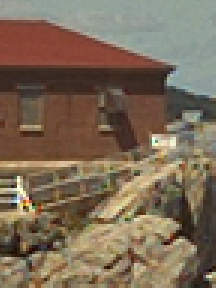
\includegraphics[width=0.3\textwidth]{figures/debayer/house_hamilton.png}} &
        \subcaptionbox{Malvar-He-Cutler (PSNR=31.15)}{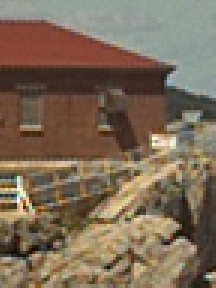
\includegraphics[width=0.3\textwidth]{figures/debayer/house_malvar.png}}
    \end{tabular}
    \caption{Coefficient values used by Malvar-He-Cutler scaled by 8 \cite{getreuerMalvarHeCutlerLinearImage2011}}
\end{figure}
\section{Digital image representations}
As with everything else that is stored on a computer, images are encoded as a sequence of bits.
RGB images are popular representations, where each pixel is stored as three sequential bytes representing each color.
This representation is very intuitive and easy to understand, but other representations might be more suitable for certain applications.

\section{Luminance and chrominance}
In many use cases, each pixel's luminance (brightness) contains more helpful information than its chrominance (color), and separating these two components is beneficial.
This is relevant for visualization, as the human eye is more sensitive to changes in luminance than chrominance  \cite{lambWhyRodsCones2016}.
It can also apply to computer vision applications, where Lucas-Kanade is an example of an optical flow algorithm that only uses the luminance component \cite{lucasIterativeImageRegistration1981}.

YCbCr
\footnote{In the computer industry, the term YUV is widely used to refer to colorspaces that are encoded using YCbCr.}
is a popular color format where the Y component represents the luminance of the pixel, while the Cb and Cr components represent the blue-difference and red-difference chrominance information respectively, as depicted in Figure \ref{fig:ycbcr_example}.

\begin{figure}[H]
    \centering
    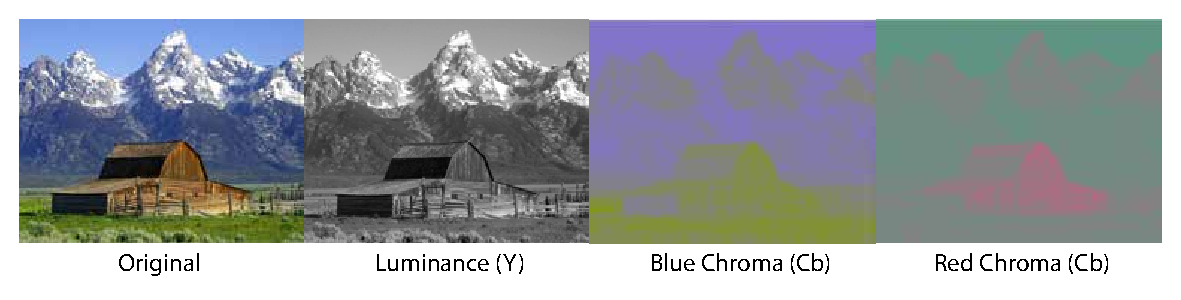
\includegraphics[width=\textwidth]{figures/debayer/YCbCr_example.pdf}
    \caption{Visualization of channels in a YCbCr image \cite{photoEnglishJohnMoulton2004}.}
    \label{fig:ycbcr_example}
\end{figure}

\subsubsection{Chroma subsampling}
Chroma subsampling is a technique that involves sampling the chrominance components (Cb and Cr) at a lower resolution than the luminance component (Y), as depicted in Figure \ref{fig:chroma_subsampling}.
A commonly used subsampling scheme is 4:2:0, where the chrominance components are sampled at half the resolution of the luminance component in both the horizontal and vertical directions \cite{ChromaSubsampling2023}.

During the process of debayering, redundant information is generated as each pixel in the output image contains three color channels, compared to only one in the raw Bayer image.
With this redundancy it is reasonable to perform chroma subsampling as the luminance component is sampled at every pixel, while a group of four pixels is required to obtain color information

\begin{figure}[H]
    \centering
    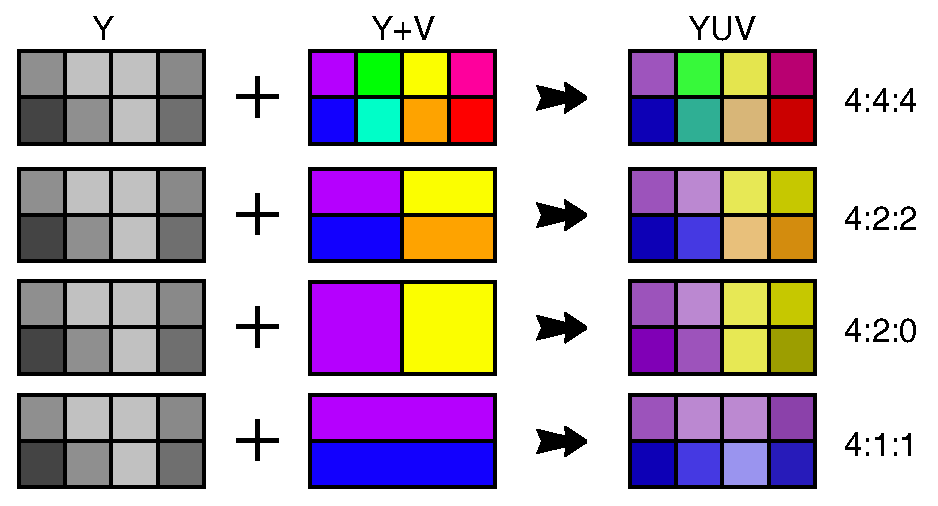
\includegraphics[width=.6\textwidth]{figures/debayer/chroma_subsampling.pdf}
    \caption{Chroma subsampling \cite{stevo-88EnglishMostWidely2010}.}
    \label{fig:chroma_subsampling}
\end{figure}


\subsection{Analog legacy}
It is important to note that certain color formats have their origins in the analog signal era.
One notable example is the BT.601 color format, a variant of YCbCr.
In this format, the Y component is represented by values ranging from 16 to 235, while the Cb and Cr components range from 16 to 240 \cite{YCbCr2023}.
The additional headroom and foot room within the byte is specifically allocated to accommodate transient signals, such as filter overshoots, and prevent undesirable effects like clipping \cite{Rec6012023}.
By reserving these values, the color representation remains within acceptable limits even when unexpected analog signal fluctuations occur.


\section{Interleved, Planar and Semi-Planar Packaging}
There are three main ways to store the color channels in memory, interleaved, planar and semi-planar \cite{baranYUVFormats2018}.
In interleaved formats, the color channels are stored in sequence, i.e.
$R_1 G_1 B_1 R_2 G_2 B_2 R_3 G_3 B_3$.
In planar formats, the color channels are stored in separate arrays, i.e.
$R_1 R_2 R_3 B_1 B_3 B_2 G_1 G_2 G_3$.
Semi-planar formats are a mix of the two where some channels are interleaved, and some are planar, i.e.
$R_1 R_2 R_3 G_1 B_1 G_2 B_2 G_3 B_3$.
The reson one might be preferred over the other is to optimize for memory locality.
For instance, if you are performing per-bit operations, having the bits of the same color channel next to each other is beneficial.

\begin{figure}[H]
    \centering
    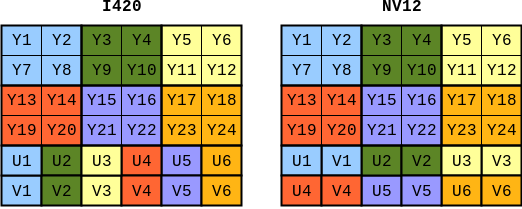
\includegraphics[width=.8\textwidth]{figures/debayer/YUV_packaging.png}
    \caption{Visualization of I420 and NV12, two popular YUV 4:2:0 formats with planar and semi-planar packaging respectively \cite{baranYUVFormats2018}.}
    \label{fig:image_packaging}
\end{figure}

\subsection{Bit depth and packaging}
A final important property of image formats is the bit depth, i.e.
how many bits are used to represent each pixel, and how the bits are stored.
Most images use a single byte (8 bits) for each color channel, but higher bit depths offer better color fidelity and dynamic range.
If the number of bits is not divisible by 8, like for 10-bit images, the most space-efficient way to store and send them is to pack them into 8-bit bytes, i.e.
four 10-bit values are stored in 5 bytes.
However, as most \glspl{alu} does not support 10-bit operations, padding to the nearest full byte is better for computations.
\section{Image data formats}
How we represent the image data in memory is another important property of image formats and can be very important for performance.
As everything else, images are encoded as a sequence of bits.
Normal RGB images are encoded as three 8-bit values for each pixel, one for each color channel.



\subsection{}



\section{Implementation}


\subsection{Reuse optimization}
The current \gls{mhc} method requires six lines of the image to be available in local memory for efficient operation.
Techincally it woulb be possible to use only five, but this would result in more cumb

\subsection{Efficient Separation}
The \gls{volta} has 48KiB of available shared memory per block \cite{rigerunNVIDIAJetsonXavier2023}.
With an image width of 2448 pixels \cite{lucidvisionlabsTriton0MPPolarization} it is only possible to store 10 lines in local shared memory.
\begin{align}
    \frac{48Kib}{2448px/line * 16b/px} = \frac{393216b}{39168b/l} \approx 10.039line
\end{align}


\begin{figure}[H]
    \centering
    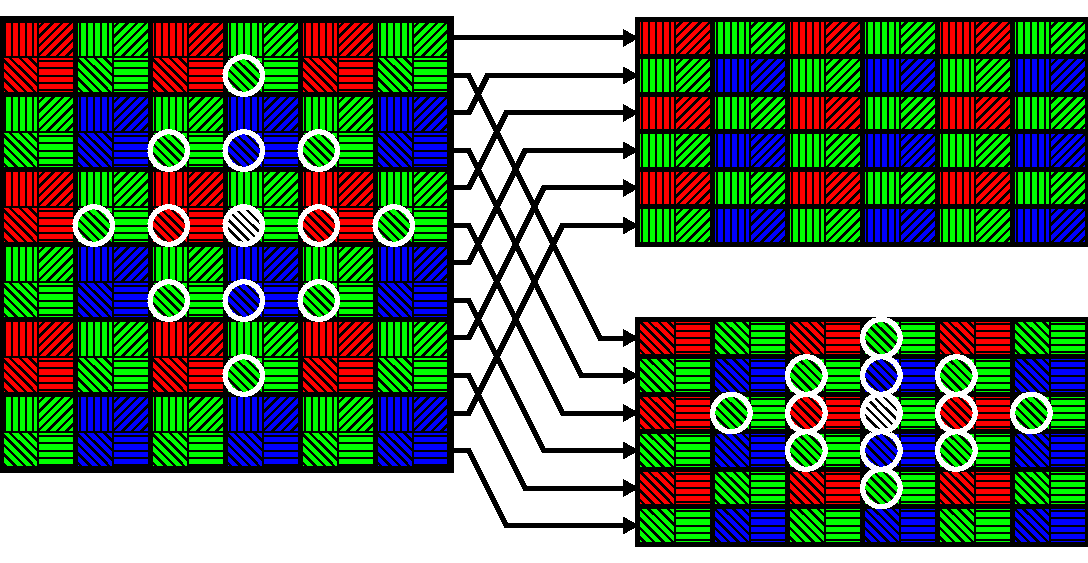
\includegraphics[width=\textwidth]{figures/polarized_image/separation.pdf}
\end{figure}

\begin{figure}[H]
    \centering
    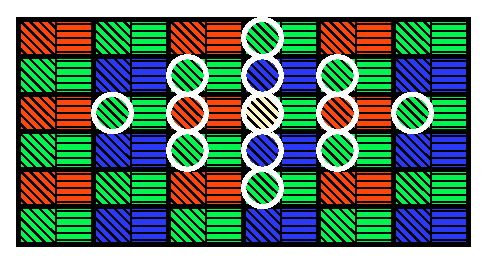
\includegraphics[width=.6\textwidth]{figures/polarized_image/separated_conv.pdf}
\end{figure}




With a runtime of $1 ms \pm 1 \mu s$
Nsight compute not working for memory







\subsubsection{Use of constant memory}
During the development process it was tested whether storing the constant values used in the debayer algorithm in constant memory would speed up the process.
Constant memory is a type of limited read-only memory available on NVIDIA \glsps{gpu} \cite[61]{nvidiaCUDABestPractices2023}.
NVIDIA \glspl{gpu} only have 64KiB of constant memory \cite[61]{nvidiaCUDABestPractices2023}.
Read instruction from constant memory are very efficient and the best performance is acheived when all threads in a warp, as opposed to regular memory where this would result in inefficient collisions \cite[61]{nvidiaCUDABestPractices2023} \cite[13,14]{volkovLatencyHiding2016}
As the different threads in each warp would need the same constants this is ideal.

All unique constant variables used in the algorithm were collected as a part of the automatic code generation and stored in a constant device array.
Unfortynately this change had no visible impact on the performance.
A minimal test was later created that performed a very simple repeated multiply and add operation, where the coefficient and constats were either stored in constant memory or defined expicitly in the funciton as shown in \code{mfa_1} and \code{mfa_2} in Listing \ref{listing:cuda_mem_tests}.
This minimal tests showed that using constant memory was actually marginally slower (0.08\% on average) than using explicit values.

Further it was tested weither the compiled code would beform better if the values in local constant variables as in the \code{mfa_3} function in Listing \ref{listing:cuda_mem_tests}.
This gave marginally better results than \code{mfa_1} (0.04\% on average), but was deemed unecessery to implement.

\begin{listing}[H]
    \begin{minted}{cuda}
        __device__ __forceinline__ __half2 mfa_1(__half2 a) {
        return __hfma2(__float2half2_rn(0.098f), a, __float2half2_rn(3.14f));
        }
        __device__ __forceinline__ __half2 mfa_2(__half2 a) {
            return __hfma2(constant_mem[0], a, constant_mem[1]);
        }
        __device__ __forceinline__ __half2 mfa_3(__half2 a) {
            const __half2 b = __float2half2_rn(0.098f);
            const __half2 c = __float2half2_rn(3.14f);
            return __hfma2(b, a, c);
        }
    \end{minted}
    \caption{Small functions used to test local memory implementations.}
    \label{listing:cuda_mem_tests}
\end{listing}



\subsection{Better reading}
Another improvement was to use an array of pointers, rather than an array of arrays.
Initially the the section of the image on which calculations were performed were stored as an array of arrays in local shared memory.
When the computations on that part was performed, the whole block would move down.
\begin{figure}[H]
    \centering
    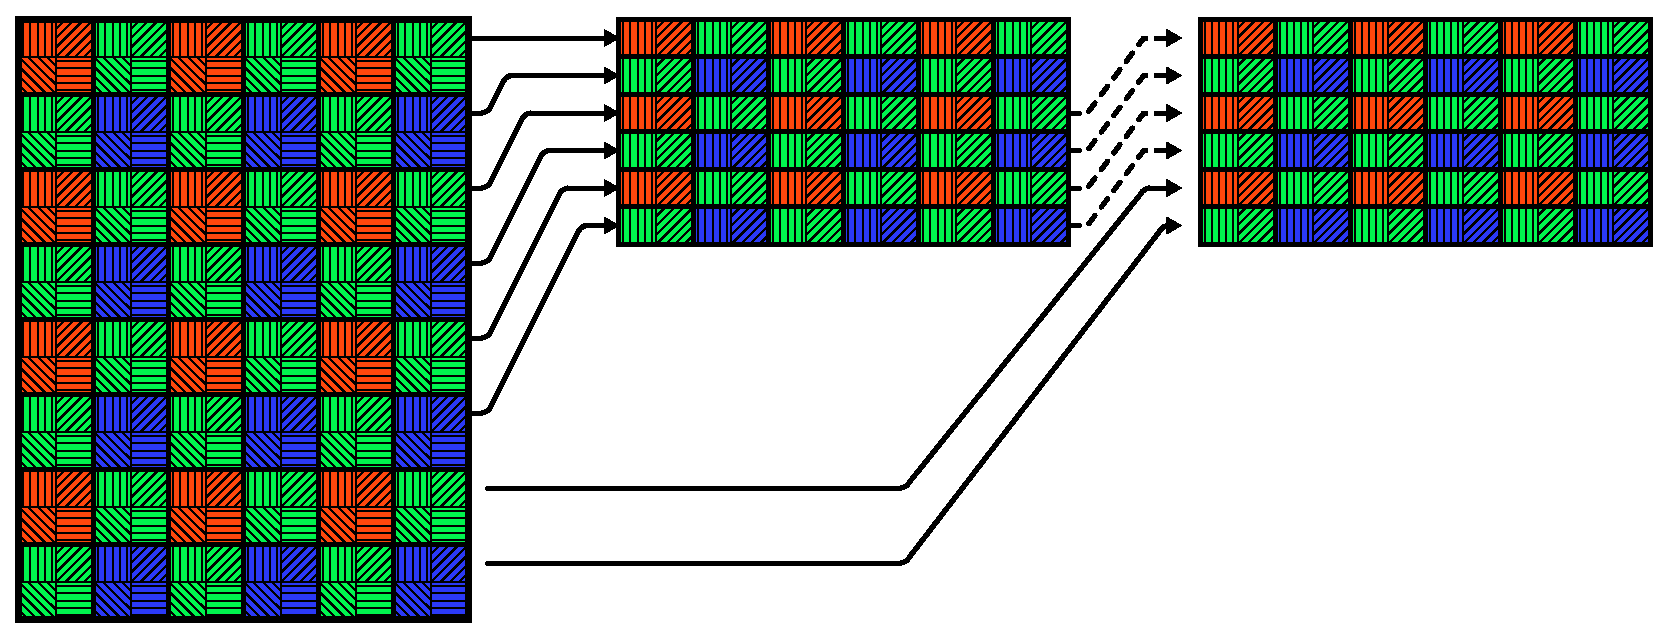
\includegraphics[width=\textwidth]{figures/polarized_image/read_line.pdf}
    \caption{TODO}
\end{figure}


\subsection{Half precitions floating point}
\section{Half-precision floating-point numbers}





\begin{figure}[H]
    \centering
    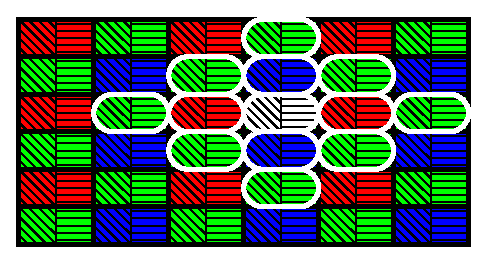
\includegraphics[width=0.45\textwidth]{figures/polarized_image/half2_conv.pdf}
    \caption{TODO}
    \label{fig:}
\end{figure}
\subsection {Unpacking raw data from the camera}
\label{sec:unpacking}


The \lucid cameras feature a 12-bit \gls{adc} and offer 23 different output formats with varying bit depths and packing.
As the \gls{h265} encoder supports up to 10-bit input, the \code{Mono10p} output format was chosen for the cameras \cite[17 ]{nvidiaNVIDIAJetsonAGX2019}
This format densly packs the 10-bit data, as depicted in Figure \ref{fig:mono10p}, maximizing the network throughput.

\begin{figure}[H]
    \centering
    \subcaptionbox{Pixel data.}{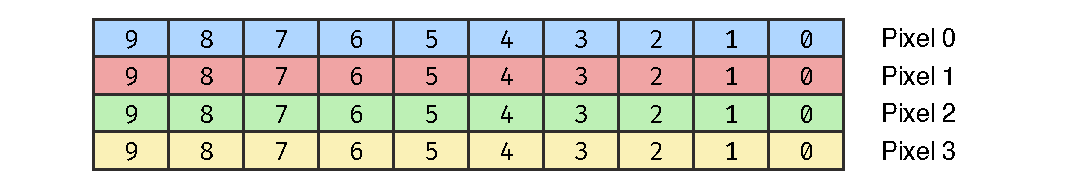
\includegraphics[width=\textwidth]{figures/unpacking/layout_10p.pdf}}
    \subcaptionbox{Bytes sent over ethernet.}{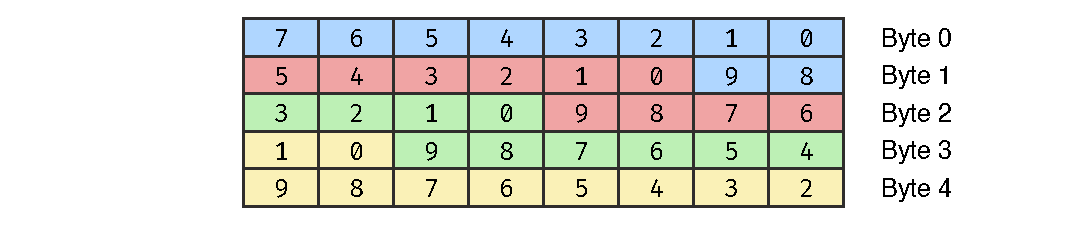
\includegraphics[width=\textwidth]{figures/unpacking/layout_10p_sent.pdf}}
    \caption{Bit layout of the \code{Mono10p} format.}
    \label{fig:mono10p}
\end{figure}


I encountered difficulties in locating documentation regarding the bit ordering on Lucid's website.
As a workaround, I relied on two test images provided by the \cam.
These test images contained pixel values that increased monotonically, as depicted in Figure \ref{fig:test_pattern}.
By analyzing the data in the first line these images, I was able to deduce the bit ordering.
Regrettably, I later discovered that Lucid Vision does provide documentation on pixel formats; however, it did not appear in their own search engine for unknown reasons \cite{lucidvisionlabsPixelFormatsLUCID2020}.

\begin{figure}[H]
    \centering
    
\includegraphics[width=0.4\textwidth]{figures/unpacking/test_pattern0.jpg}
    
\includegraphics[width=0.4\textwidth]{figures/unpacking/test_pattern2.jpg}
    \caption{Two test images used to infer the bit ordering.
        The \cam can output several different test patterns useful for various testing purposes \cite{lucidvisionlabsTritonMPPolarized2020}.}
    \label{fig:test_pattern}
\end{figure}


\subsubsection{Bit unpacking} \label{sec:contuguous_access}
The pattern in Figure \ref{fig:mono10p} was identified as being little endian, meaning the least significant bytes is stored first.


\subsubsection{Contiguous acces using warp level primitives} \label{sec:contuguous_access}
As we want to operate on 32-bit values and each pixel is stored as a 10bit value, each thread is processing 160 bits, or five words as it is the lowest common multiple of 32 and 10.
Thus every thread reads five consecutive words as shown:
\begin{align}
    a_T[i] = d[T*5+i], &  & i \in (0,1,2,3,4)
\end{align}
Where $T$ is the thread intex in the warp, $a_T$ is local memory of thread $T$, $d$ is the image stored in device memory, and $k$ is some constant offset.






It was hypothized that it would be faster to let first read the data contiguously into shared memory and then redistribute it as follows:
\begin{align}
    s[i*32+T] & = d[i*32+T],  & i & \in (0,1,2,3,4) \\
    a_T[i]    & = s[(T*5+i)], & i & \in (0,1,2,3,4)
    \label{eq:contiguous_reading}
\end{align}
Where $s$ is shared local memory of thread, but this was slower than the initial uncoalesced reading.


A secont attmempt was done using the \code{__shfl_sync} function which is a warp-level primitive used to exchange data between threads in a warp \cite{linUsingCUDAWarpLevel2018}.
As the data exchange is performed directly between registers this is faster than going through shared memory \cite{linUsingCUDAWarpLevel2018}
Data was read contiguously into local buffers of each thread, then exchanged so every thread ended up with five consecutive words.
However finding the right indices is hard as you need specity what data to send and what thread to read from, rather than what data to read from what thread.
The full index table, shown in Table \ref{table:memory_index} in Appendix \ref{chap:additional_resources}, was created and studied in order to end up with the following formulation:
\begin{align}
    c_T[i] & = d[i*32+T],       &   &                   & i & \in (0,1,2,3,4) \\
    c_T[j] & \rightarrow a_x[i] & j & = (2 * (T -i))\%5 & i & \in (0,1,2,3,4) \\
    a_T[i] & \leftarrow c_j[x]  & j & = (T*5 + i)\%32   & i & \in (0,1,2,3,4)
    \label{eq:contiguous_reading_shfl}
\end{align}
where $x$ represents the thread the data is sent to.
The code equivalent to this is written as follows.
\begin{minted}{cuda}
    a[i] = __shfl_sync(0xffffffff, c[2(*(T-i))%5], (T*5 + i)%32);
\end{minted}

\section{Profiling}

\subsection{Nsight Compute}
\begin{figure}[H]
    \centering
    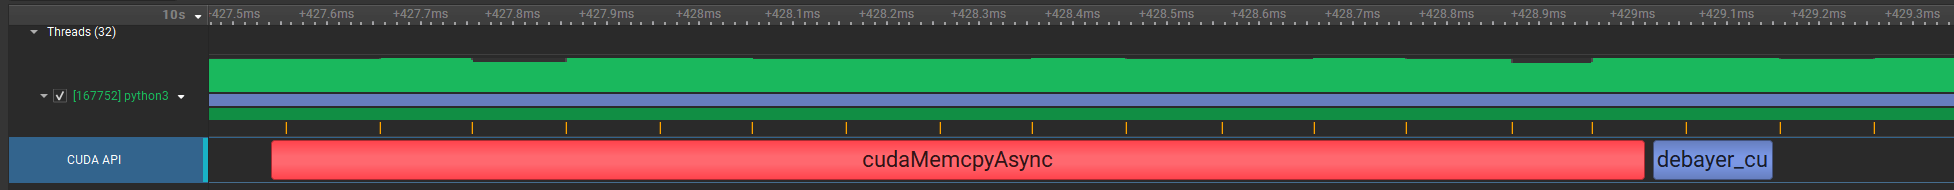
\includegraphics[width=\textwidth]{figures/memory_comparaison.png}
\end{figure}

\subsection{Memory profiling}
Pinned memory does not work


\begin{listing}[H]
    \begin{minted}{python}
        class Myprinter(CXX11CodePrinter):
            def _print_Indexed(self, expr: sp.Indexed):
                return f"{expr.base}[{expr.indices[0]}][{expr.indices[1]}]"

            def _print_Float(self, expr):
                return f"__float2half2_rn({expr:.9e}f)"

            def _print_Add(self, expr: sp.Add):
                args = list(expr.args)
                toadd = []
                out = ""
                for i, el in enumerate(args):
                    if isinstance(el, sp.Float):
                        toadd.append(el)
                        continue
                    assert isinstance(el, sp.Mul) and len(el.args) == 2
                    arg0 = self._print(el.args[0] / 1024)
                    arg1 = self._print(el.args[1])
                    if i == len(args) - 1:
                        out += f"tmp =__hfma2_sat({arg0}, {arg1}, tmp);\n"
                    else:
                        out += f"tmp =__hfma2({arg0}, {arg1}, tmp);\n"
                out = f"__half2 tmp = {self._print_Float(sum(toadd))};\n" + out
                return out
        \end{minted}
    \caption{Code printer to perform multiply and add operations on \halftwo}
\end{listing}

% tmp = __hfma2(__float2half2_rn(1.801812744e-4f), data[3][col + 1], tmp);
% tmp = __hfma2(__float2half2_rn(9.701843262e-6f), data[2][col + 3], tmp);
% tmp = __hfma2(__float2half2_rn(9.701843262e-6f), data[5][col], tmp);
% tmp = __hfma2(__float2half2_rn(1.483016968e-5f), data[3][col + 3], tmp);
% tmp = __hfma2(__float2half2_rn(1.483016968e-5f), data[5][col + 1], tmp);
% tmp = __hfma2(__float2half2_rn(2.661132812e-5f), data[1][col - 1], tmp);
% tmp = __hfma2(__float2half2_rn(-4.560012817e-5f), data[3][col + 2], tmp);
% tmp = __hfma2(__float2half2_rn(-4.560012817e-5f), data[4][col + 1], tmp);
% tmp = __hfma2(__float2half2_rn(-2.799591064e-5f), data[2][col + 2], tmp);
% tmp = __hfma2(__float2half2_rn(-2.799591064e-5f), data[4][col], tmp);
% tmp = __hfma2(__float2half2_rn(-1.025665283e-5f), data[1][col + 2], tmp);
% tmp = __hfma2(__float2half2_rn(-1.025665283e-5f), data[4][col - 1], tmp);
% tmp = __hfma2(__float2half2_rn(-8.205322266e-5f), data[2][col + 1], tmp);
% tmp = __hfma2(__float2half2_rn(-8.205322266e-5f), data[3][col], tmp);
% tmp = __hfma2(__float2half2_rn(-6.098022461e-6f), data[4][col + 2], tmp);
% tmp = __hfma2(__float2half2_rn(-9.701843262e-6f), data[0][col], tmp);
% tmp = __hfma2(__float2half2_rn(-9.701843262e-6f), data[2][col - 2], tmp);
% tmp = __hfma2(__float2half2_rn(-1.483016968e-5f), data[0][col + 1], tmp);
% tmp = __hfma2(__float2half2_rn(-1.483016968e-5f), data[3][col - 2], tmp);
% [firstnumber=5]
%         % tmp = __hfma2(__float2half2_rn(-1.607482910e-5f), data[2][col], tmp);
%         % tmp = __hfma2(__float2half2_rn(-2.106811523e-5f), data[1][col], tmp);
%         % tmp = __hfma2_sat(__float2half2_rn(-2.106811523e-5f), data[2][col - 1], tmp);
%         % return __hfma2(__float2half2_rn(1023.0f), tmp, __float2half2_rn(0.0f));
\begin{listing}[H]
    \begin{minted}{cuda}
        __device__ __forceinline__ __half2 handle_u(__half2 **data, int col) {
            __half2 tmp = __float2half2_rn(5.000000000e-1f);
            tmp = __hfma2(__float2half2_rn(9.466415405e-5f), data[1][col + 1], tmp);
            tmp = __hfma2(__float2half2_rn(9.466415405e-5f), data[3][col - 1], tmp);
        \end{minted}
    \vspace{-26pt}
    \begin{minted}[linenos=false, autogobble=false]{cuda}
    ...
    \end{minted}
    \vspace{-26pt}
    \begin{minted}[firstnumber=24]{cuda}
        tmp = __hfma2(__float2half2_rn(-1.122532265e-5f), data[0][col], tmp);
        tmp = __hfma2_sat(__float2half2_rn(-1.122532265e-5f), data[2][col - 2], tmp);
        return __hfma2(__float2half2_rn(1023.0f), tmp, __float2half2_rn(0.0f));
    }
    \end{minted}
    \caption{Generated function}
\end{listing}

\subsubsection{Issue with max value}
\subsection{Color space conversion}

\subsection{Packaging}
\chapter*{Video Processing with GStreamer}
\label{chap:gstreamer}
\section{Motivation}
A significant amout of work was put into enabling on the fly compression of the videostreams from the \sr.
That is the ability to compress the video data as it is being recorded, and storing the compressed data on disk.

The sensor rig produces roughly 2Gib of data per second with a stereo camera setup.
At this rate, it will only take x days to produce a terabyte of data.
\begin{align}
    \frac{1\text{TB}}{2\text{Gb/s}} & = \frac{1\text{TB}}{0.25\text{GB/s}} \\
                                    & = 4000\text{s}                       \\
                                    & \approx 1\text{h} + 7\text{min}
\end{align}

It can be argued that datasets of this size is good enough, especially since it would also be possible to an \gls{ssd} with a capacity up to 8TB \cite{CorsairMP600PRO}, enabling roughly 9 hours of recording.
However, there are three reasons why on the fly compression is desirable:
If the sensor rig is mounted on a ship, it will be possible to transfer all the data to a storage server on the ship over regular ether net, using the ethernet port on the \jx which is limited to 1Gb/s.

By adjusting the compression rate of the sensor rig data can be transferred over ethernet for remote real time processing.
The compression has to be done at some point anyway.







\subsection{Visualization}
A usefull way debug \gs applications is to generate visualizations of the pipeline.
To acheive this the environe ment variable \code{GST_DEBUG_DUMP_DOT_DIR} must be defined and the \code{GST_DEBUG_BIN_TO_DOT_FILE} macro needs to be executed on the final graph if it is part of a custom GStreamer application, whic is the case on the \sr.
\cite{johnstonGeneratingGStreamerPipeline2018}
This will generate temprorary information \textit{.dot} files that can later be converted to visualized graphs using \gls{gviz}.
Figure \ref{fig:gs_pipeline_visualization} shows the final graph that is used on the \sr.
It has been modified in Adobe Illustrator to be more compact, but is still to large to b


\begin{figure}[H]
    \centering
    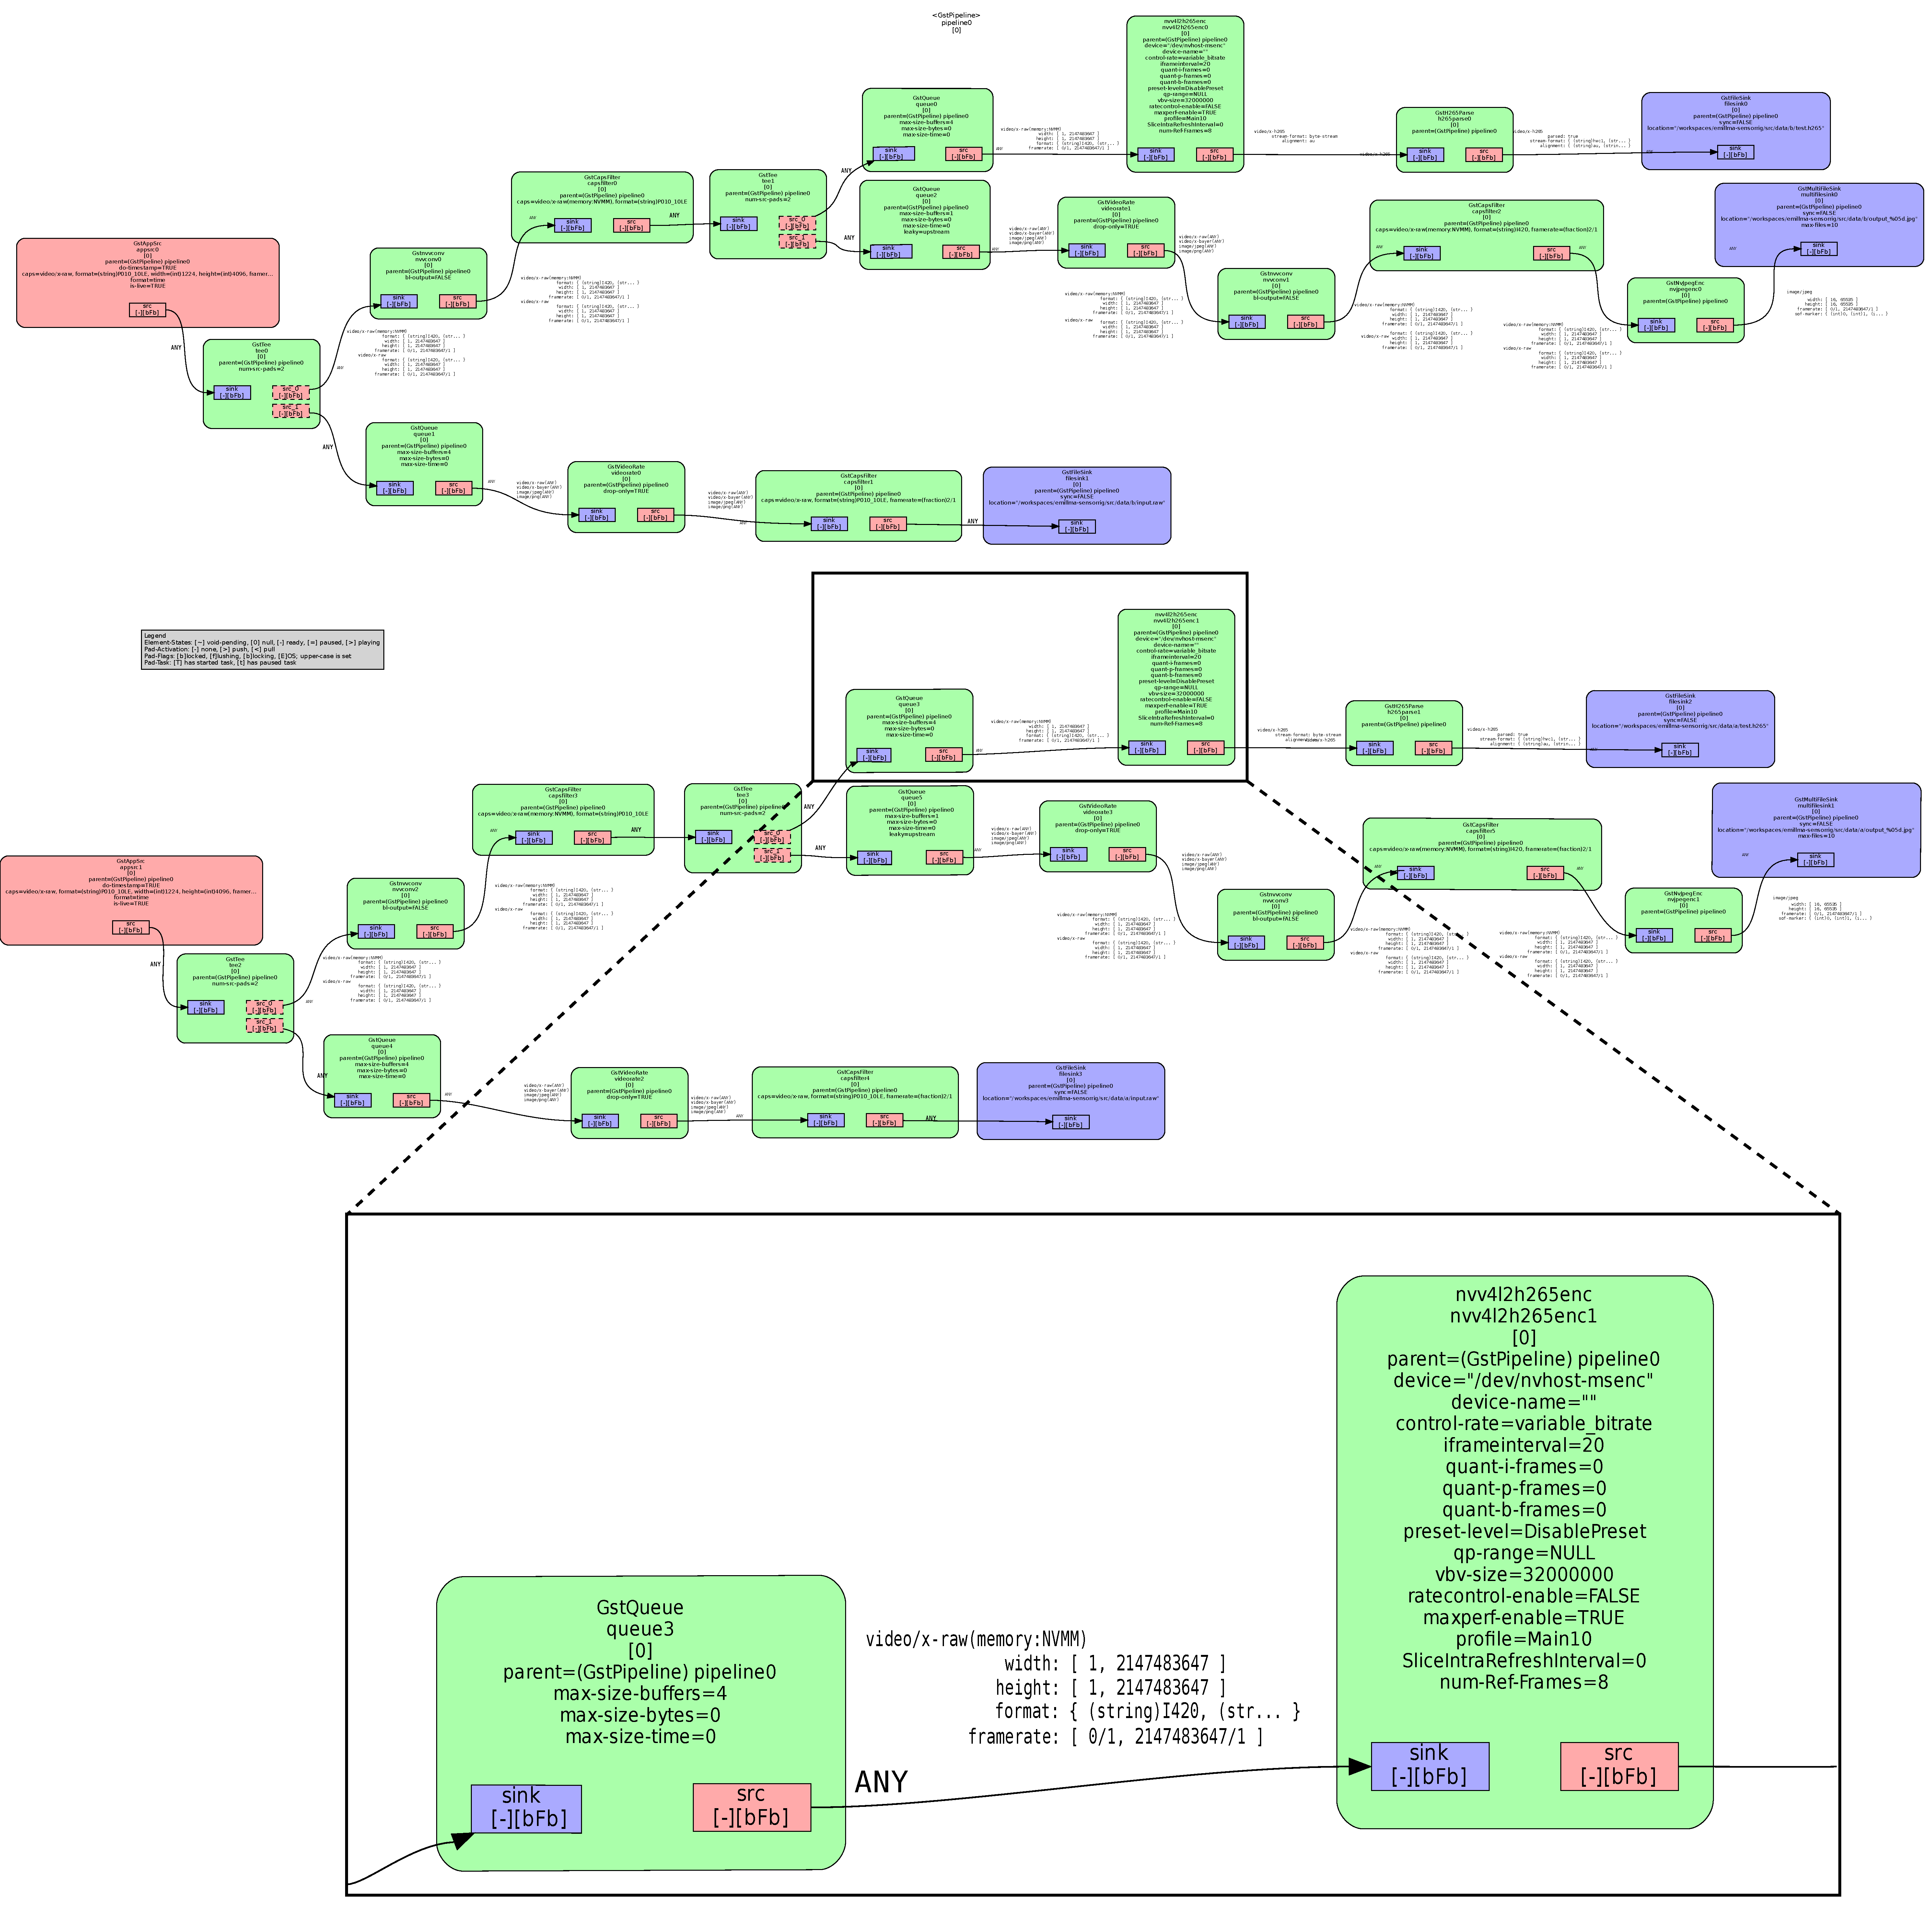
\includegraphics[width=\textwidth]{figures/pipeline.pdf}
    \caption{Visualization of the \gs Pipeline used on the \sr.
        The graph was crated using GraphViz and edited in Adobe Illustrator to be more compbact and readable. The bottom part shows a zoomed in version of the encoder part of used on the second camera.}
    \label{fig:gs_pipeline_visualization}
\end{figure}
\section{GStreamer in Python}

\subsection{PyGobject}
\subsection{Stubs}

\cite{pygobjectTypingStubsPyGObject2023}
\section{Communicating with GStreamer Pipeline}
The easiest way to use \gs is to use \code{gst-launch-1.0} from the terminal, a tool that builda and runs basic \gs pipelines from a pipeline description string \cite{Gstlaunch1}.
An extensive list of examples on how to use \code{gst-launch-1.0} can has been made by Adrian Lane and can be found on his GitHub \cite{laneGStreamerPipelineSamples2020}.

Initially \code{gst-launch-1.0} was used to create pipelines to compress the images to \gls{h265} video streams and \gls{jpeg} images.
Different approaches were tested for communicating with the generated pipeline from Python.

\subsection{Method 1: Regular and temporary files}
A very simple and naive way to communicate with the pipeline is to use files.
The imput images were saved to files and the pipeline was set up to read from that file.
The opposite was done to get the output images.
When using regular files this approach was slow and not very reliable.
Using \gls{tmpfs}, which makes it possible to store temporary files in \gls{ram} instead of on disk improved the performance, but it still felt like a very naive approach \cite{dickinsTmpfsLinuxKernel2010}.

\subsection{Method 2: Network protocols}
The first approach to transfer the images was to send and receive data over the network.
\gs has both a \gls{tcp} client source and \gls{tcp} server sink that can be used to pipe data to the pipeline as well as from the pipeline.
Using \gls{tcp} was easy to set up and worked quite well as the pipeline could run independently in one process while a server serving input data and a output data client could run anywhere else, even on another computer on the same network.
The server an client were implemented in Python using the \gls{asyncio} library.
Using \gls{udp} was also tested and appeared to perform equally well, but made it impossible to monitor weither the pipeline was running properly and if any client were actually receiving data.


\subsection{Method 3: STDIN and STDOUT}
Another approach was to use \gls{stdin} and \gls{stdout} to pipe data to and from the pipeline.
\gls{asyncio}.
This approach is very similar in nature as using files, as \gls{stdin} and \gls{stdout}, like almost everything else in Linux, are represented as files \cite{mckayWhatAreStdin2020}.
However this approach is more elegant as it does not require any files and designed for this exact purpose.
The \gs process was started using \gls{asyncio} to be able to read and write to \gls{stdin} and \gls{stdout} asynchronously.


\section{Parsing of JPEG bytestream}
Initially the data generated from \gs was piped through \code{stdout}.
The following binary \gls{regex} was used in to separate the images.
\begin{figure}[H]
    \centering
    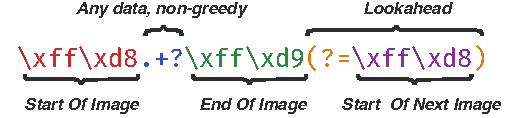
\includegraphics[width=0.7\textwidth]{figures/jpeg_regex.pdf}
\end{figure}
It looked for the beginning marker followed by data followed by the end marker and with a lookahead for the beginning marker of the next image.
The final lookahead was used to minimize the chance of parsing data bytes as the end marker as it was believed that could happen.
After analyzing the \gls{jpeg} standard however it was discovered that they use a technique called byte stuffing which ensures this never happens \cite[91]{ccittINFORMATIONTECHNOLOGYDIGITAL1992}.
Byte stuffing is a technique used in data transmission where special control characters are inserted into the data stream to distinguish between data and control information.
For \glspl{jpeg}, the zero byte is inserted after every control character that appears in the data \cite[91]{ccittINFORMATIONTECHNOLOGYDIGITAL1992}.
This made the parsing could be done both easier and faster by simply reading until the end-of-image marker.

\chapter{Pipeline Assembly in Python}
\label{chap:pipeline}
This chapter links the preceding three chapters, illustrating assembling the different components into a functional pipeline.
An outline of the pipeline's operation and a discussion on certain design choices is presented.
The complete source code is available upon request.

% \section{Approach to Concurrency}
% As discussed in \ref{sec:concurrent_programming_in_python} using \gls{asyncio} is performant than using threads and offers more control over the execution and is therefore used to implement the pipeline.
% When the execution of external blocking code is required, it is wrapped in a \code{run_in_executor} call to run it in a thread pool.
% \gls{pygo} is callback-based,

% Several design patterns were tested during the development of the pipeline.
% In the final implementation

\section{Overall Structure}
The pipeline includes a synchronous setup phase, a concurrent running phase for executing multiple tasks, and a teardown phase for graceful shutdown of all tasks.
Figure \ref{fig:object_overveiw} provides a high-level overview of the object in the pipeline and their interactions.

\gls{asyncio} is used to implement the concurrent running phase when possible, but certain tasks and callbacks are run in separate threads as this is required by some of the libraries used.


\subsection{Setup Phase}
\label{sec:discovery}

During the setup phase, the network manager ensures the Ethernet devices are configured as discussed in Section \ref{sec:network_configuration}.

Next, the camera manager is initialized to discover and configure the cameras.
Each Ethernet device has its own subnet where it attempts to find cameras.
If no cameras are detected, it searches the \gls{lla} subnet and configures any discovered camera to use an IP address within its subnet.

Once the cameras have been successfully discovered and configured, the Debayer Manager and GStreamer Manager, along with their respective pipelines, are initialized.

Finally, the video streams are initialized, and the running phase begins.

\subsection{Running Phase}
During the running phase, there are multiple concurrent tasks:

\begin{itemize}
    \item The \gls{ptp} Trigger continuously sends triggering signals to the cameras for simultaneous frame capture.
    \item Each Frame Grabber continuously grabs frames from the cameras and stores them in a queue.
    \item The Debayer Manager continuously retrieves frames from the queues, runs the debayer kernel, and stores the output in a thread-safe queue.
    \item The Sink Pads, using callbacks, read data from the queues and pass it to the corresponding Pipeline when data is requested.
    \item The Src Pads, also using callbacks, pass available \gls{jpeg} data from the Pipeline to another thread-safe queue.
    \item An asynchronous \gls{ws} client forwards the \gls{jpeg} data to the PubSub Server discussed in Section \ref{sec:pubsub}.
    \item Another client listens to various camera setting topics and configures the cameras accordingly.
    \item The GStreamer Manager runs in a separate thread.
\end{itemize}



\subsection{Shutdown Phase}

When the pipeline receives a shutdown signal from the \srgui via the PubSub Server, it initiates the shutdown phase.
All tasks are instructed to stop, and the pipeline waits for their completion before terminating any remaining tasks.
Subsequently, the memory is freed, the streams are closed, and the \gls{ws} clients are disconnected.
The network settings and camera settings are not resotred to minimize the startup time for subsequent runs.
Leaving the cameras with an IP withing the corresponding Ethernet device's subnet ensures that they are discovered a lot faster.


\begin{figure}[H]
    \centering
    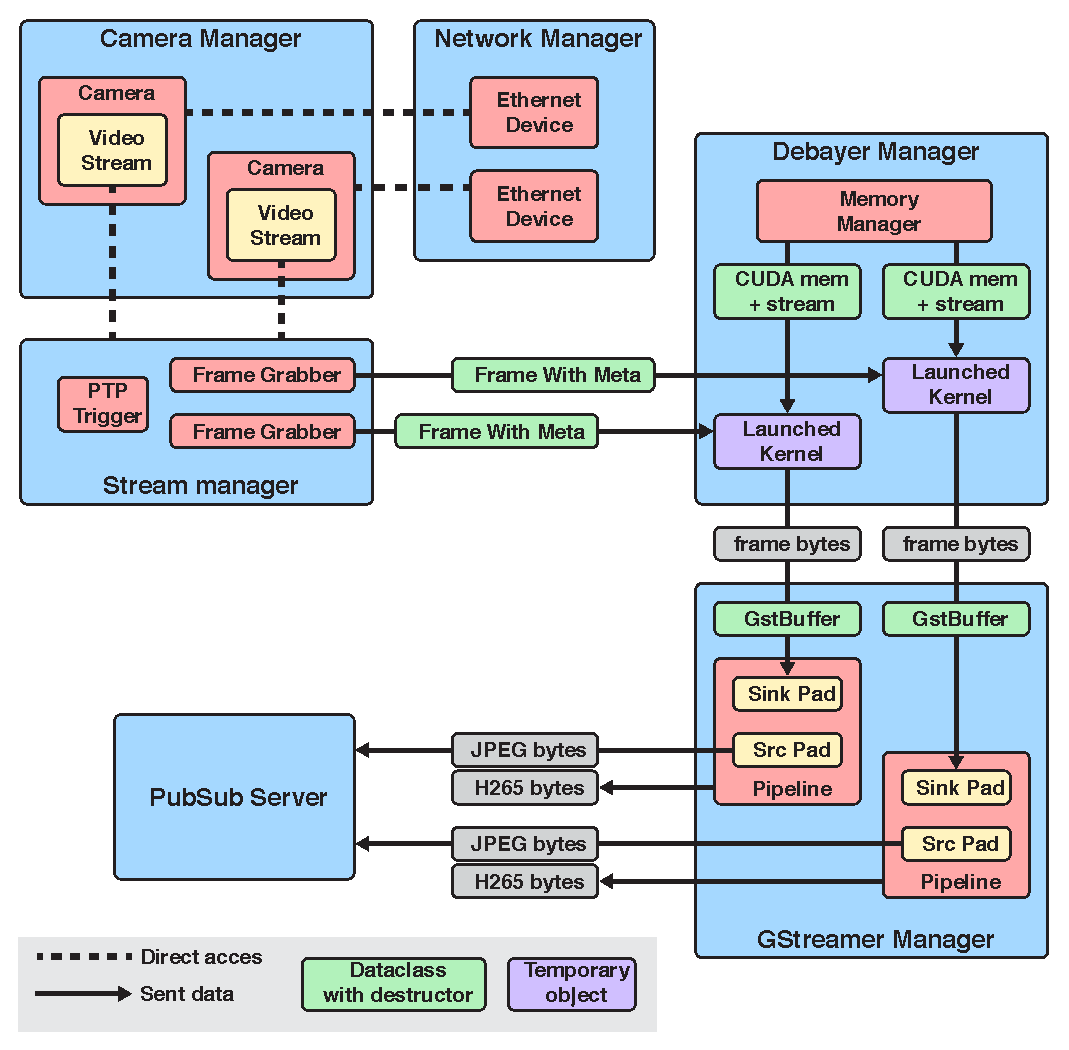
\includegraphics[width=\textwidth]{figures/object_overview.pdf}
    \caption{Class diagram showing the relationship between the classes in the pipeline and how thei interact.}
    \label{fig:object_overveiw}
\end{figure}

\section{Notes on Key Features}
Following are notes on some of the key features of the pipeline.

\subsection{Sharing Subcomponents}
To address synchronization challenges during object creation, configuration, and utilization, the pipeline employs a strategy where certain sets of elements are created, owned, and destroyed by one object but directly used by another.

The ethernet device objects are created, owned and configured by the Network Manager, and used by directly by the Camera Manager during the creation of each Camera object.
The network manger ensures that they never are configured to have overlapping subnets, as this causes issues during the discovery, creation and operation of the cameras.

The Video Stream objects are created and confibured by their corresponding camera object and used direcly by the Video Stream Manager, which grabs frames and makes sure that left and right frames are synchronized.

\subsection{Graceful Shutdown}
In real-time systems involving external hardware, it is essential to implement controlled shutdown procedures to avoid potential complications and issues in future runs.

On the \sr it is especially important to handle the camera and stream objects appropriately to avoid the cameras becoming inaccessible.
This is achieved by utilizing the \code{with} and \code{async with} syntax in Python, along with \code{try-finally} blocks, to ensure proper resource cleanup.

In case the cameras become inaccessible, a possible solution is to temporarily disable the Ethernet interface they are connected to for approximately two minutes.
This action appear to trigger an internal reset of the cameras, restoring their functionality.

\subsection{Custom Destructors}
Several custom message types have been developed with custom destructors to ensure proper cleanup.

The Frame With Meta object contains the data and relevant metadata for a single frame.
The underlying memory is managed internally by \gls{arena-api} and needs to be explicitly freed back to the underlying memory pool in order for new frames to be allocated.
This object has a custon \code{free} function used to free the underlying memory and \code{__del__} function that logs a warning if the memory has not been freed explicitly and frees it.

Allocating\gls{cuda} memory is a slow operation.
According to \gls{nsys}, allocating the tecessary memory to perform the transformation presented in Chapter \ref{chap:debayer} takes more time than the transformation itself.
To avoid this overhead a custom\gls{cuda} memory pool was implemented that r\gls{cuda} CUDA memory in order to avoid allocating and freeing memory and stream objects for each frame.
This pool is managed by the Memory Manager.
When the\gls{cuda} Memor\gls{cuda} CUDA Stream used by a kernel goes out of scope

Finally, Gstreamer uses their own garbage collecion system and reference counting to manage memory.
Fortunately the \gls{pygo} bindings for Gstreamer handles this automatically by having the python object participate in the reference counting, ensuring that the underlying Gstreamer object is not freed before the \py object is.


\subsection{Debayer Manager: Running CUDA Kernels in Python}
The main role of the debayer manager is to integrate the\gls{cuda} code with \py.
To acheive this \gls{pybind11} was used.
\gls{pybind11} is a \gls{cpp} library that allows for the creation of \py bindings for \gls{cpp}, also \gls{cpp} funcions that launch \gls{cuda} kernels.

When working with \gls{cuda} the easiest way to data from python was to pass pointers to the underlying data of the \gls{numpy} and \gls{cupy} arrays.
These pointers are available as inegers through the \code{__array_interface__} and \code{__cuda_array_interface__} respectively \cite{numpyArrayInterfaceProtocol} \cite{cupyInteroperabilityCuPy12}.
This allows for zero-copy data transfer between \gls{cuda} and \py, but requires manual interpretation of the data structure on the \gls{cpp} side and should be done with caution as it is easy to get segmentation faults.

Passing data as \gls{eigen} arrays without copying the data was also acheived and the \gls{eigen} arrays could be used directly in \gls{cuda} \cite{wenzelEigenPybind11Documentation2017} \cite{eigenEigenUsingEigen}.
While this was a more memory safe way to transfer datait requiered a lot more boilerplate on the \gls{cpp} side and was slower than passing pointers to the underlying data.


It is worth mentioning that it is also possible to write \gls{cuda} kernels in \py directly through \gls{cupy} as well as other \gls{gpu} accelerated libraries such as \gls{numba} and \gls{pytorch}
Based on prioer experience however these are impossible to debug and should be avoided for anything but the simplest of tasks.
\section{Memory Movement in the Pipeline}
Figure \ref{fig:pipeline_current} shows an overview of the memory movement in the current pipeline.
Work was put into minimizing the memory movement in the pipeline, yet there are still some redundant copies as shown in the figure.
How to remove these redundant copies is further discussed in Section \ref{sec:memory_pipeline_improvements}.

\begin{figure}[H]
    \centering
    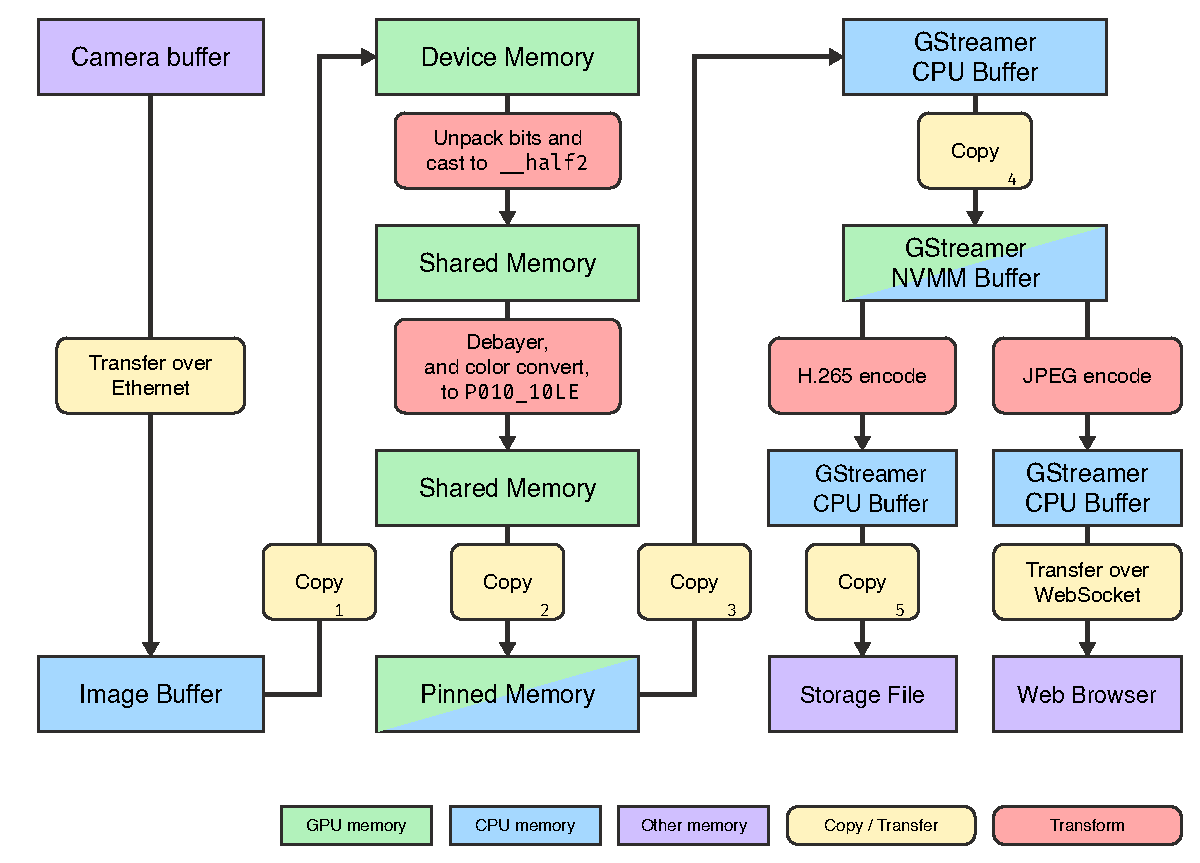
\includegraphics[width=\textwidth]{figures/memory_pipeline/current.pdf}
    \caption{Overview of the memory movement in the current pipeline.}
    \label{fig:pipeline_current}
\end{figure}




\begin{figure}[H]
    \centering
    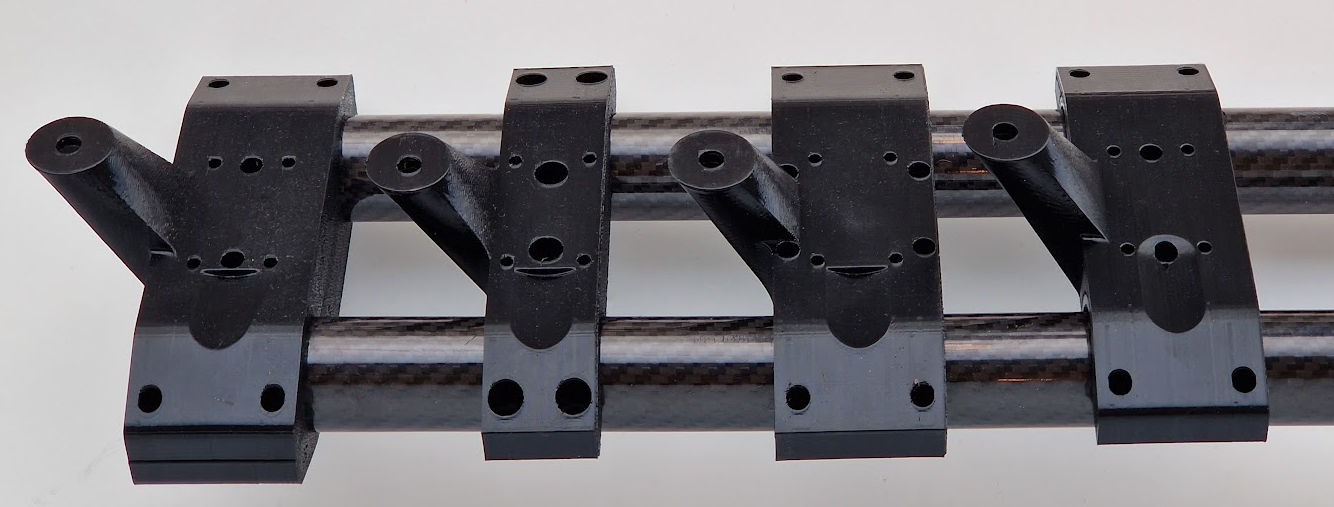
\includegraphics[width=\textwidth]{figures/3d_print/cam_mounts.png}
    \caption{Some iterations on the camera mount design}
    \label{fig:cam_mounts_iterations}
\end{figure}
\subsection{Carry grips}


\subsubsection{Motivation}
At the end of the \preproject the sensor rig was possible to carry, but the grip was not very ergonomic.
Each hand had to hold each of the carbo fiber tubes to keep it balances, but this resulted in difficult handling, especially of the pitch angle.
Furthermore, the current design relies on controlling the software from a mobile phone, which requieres one hand in short perioeds of time, making the handling even more difficult.
To solve this problem, carry gimbal grips were designed and 3D printed.


\subsubsection{Base design}
Early on it was made clear that designing an ergonomic grip from scratch would be difficult and timeconsuming as it involves a lot of difficult geometric shapes.
Thus the idea was to use an existing design as a starting point.
To find a suitable design, the following search terms and model sites were used:

\begin{multicols}{2}
    \textbf{3Dmodel sites}:
    \begin{itemize}
        \item Thingiverse
        \item Printables
        \item GrapCad
        \item Cults
        \item Free3D
    \end{itemize}
    \columnbreak
    \textbf{Key words:}:
    \begin{itemize}
        \item handle
        \item grip
        \item ergonomic handle
        \item ergonomic grip
        \item carry handle
        \item carry grip
    \end{itemize}
\end{multicols}

A well designed set of ergonomic handles were found on Ptintables \cite{matulichErgonomicHandleBased}.
The design of the handles was well documented on the creators blog page \cite{matulichWhoseHandsAre2022}
It is based on the anatomy of the human hand and the selected model had the selected model had trochoidal finger grooves, making it a good starting point for the design of the carry grips.

As the model did however not fit my hands very well, so multiple iterations were made to find a good fit.
Firstly the rough scaling needed was found by printing the outline of the grip in multiple sizes.
This was donw in "vase mode", a method where the printer prints the outline of the model in one continous spiral, to make the iteration fast \cite{ghargeCuraVaseMode2022}. One of these test prinst is shown in figure \ref{fig:handle_iteration}.

After having figured out a rough size, the whole grip was printed in in a couple of different sizes and a blind test was performed on myself and a couple of friends to find the best fit.
With the eyes closed the test subjects were asked to hold different grips and say if it was too big or too small in any direction or if it felt okay.
The same grip were given to the test subjects multiple times to make sure the results were consistent.
Based on the results of this test, a final the final design is 10\% higher, 20\% wider and 25\% deeper than the original design.

\begin{figure}[H]
    \centering
    \includegraphics[width=.8\textwidth]{figures/3d_print/handles.png}
    \caption{Iterations on carry handle design. The handle marked with a 1 was printed sideways, resulting in a bad underside. The handle marked with a 2 shows one of the many handles printed in "vase mode" for fast iteration.}
    \label{fig:handle_iteration}
\end{figure}

\subsubsection{Integration with sensor rig}

\begin{figure}[H]
    \centering
    \includegraphics[width=\textwidth]{figures/3d_print/break.png}
    \caption{Some iterations on the camera mount design}
    \label{fig:hancle_break}
\end{figure}

\begin{figure}[H]
    \centering
    \includegraphics[width=\textwidth]{figures/3d_print/thickness.png}
    \caption{Some iterations on the camera mount design}
    \label{fig:handle_thickness}
\end{figure}
\section{3D printing}
A

\subsection{Argumentation}
As the department have several 3D-printers available


\subsection{Choice of printer}
During the master thesis

\subsection{Slicer}

\subsection{Parameters}
\subsubsection{Layer height}
\subsubsection{Infill}
\subsubsection{Initial layer height}

\chapter{Sensor rig}
What is lacking in the current sensor rig.


\section{Make carry handles}
More ergonomic.

\section{Test/fix cooling}
Verify if cooling is sufficient.

\section{Camera mounts}

\subsection{3D printer}

\subsubsection{Workflow}
Having a 3D printer available changed the workflow.
Last year everything was made at OV, so if parts were 3D printed two separate trips were requiered, one to start print and one to stop it.
Test parts were therefore not really an option.
This made using the laser cutter more favorable as multiple test parts could be made in one session.

\subsubsection{Snapmaker J1}
Idex printer makes it easier to print supports.
Bambu lab X1 and Prusa were considered.
Long delay.

\subsubsection{Configuration}
Quite a lot of time was spent on configuring the printer.
Two different slicers were used, Cura and Luban.
Router was aquired for wireless transfer of files.



\chapter{Compiling NVIDIA Jetson Linux with PPS and flashing the NVIDIA Jetson Xavier}
\begin{figure}[H]
    \centering
    \includegraphics[width=\textwidth]{figures/cautionary.png}
    \caption{Cautionary by XKCD \cite{xkcdCautionary2008}}
    \label{fig:xkcd_cautionary}
\end{figure}

\section{Introduction}
To get some \gls{gstreamer} elements working, it was necessary to update the Linux Kernel on the \jx \cite{martensProblemsNvvidconvVideo2023}.


\section{PPS interrupts in Linux}
\review
\gls{pps} is a high precision signal that repeats every seconds provided by a device, typically a GPS receiver, that is used to adjust the system clock time with high accuracy \cite{giomettiLinuxPPSWikiLinuxPPS2007}.
The \gls{pps} signal is often used in combination with \gls{ntpd} to synchronize the system clock with to \gls{utc} with sub millisecond accuracy \cite{giomettiLinuxPPSWikiLinuxPPS2007}.
As \gls{pps} interrupts are hardware based it appears necessary to configure the Linux Kernel as it is responsible for handling interrupts \cite{giomettiLinuxPPSWikiLinuxPPS2007}.
The kernel is the core software component of an operating system that manages system resources and provides a bridge between software applications and hardware devices as visuzlized in Figure \ref{fig:kernel_visualization} \cite{thekerneldevelopmentcommunityInterruptsLinuxKernel}.
On the \sr a \gls{pps} signal from one of the \glsps{f9p} is used to sunchronize the clock on the \jx to \gls{utc}, which again is used to synchronize of the cameras using \gls{ptp} \cite{martensPortableSensorRig2022}.

\begin{figure}[H]
    \centering
    \includegraphics[width=\textwidth]{figures/kernel.pdf}
    \caption{An oversimplification of who the kernel interacts with the hardware and software}
    \label{fig:kernel_visualization}
\end{figure}

\section{Jetpack}
\review
The \jx runs an operating system called \gls{jetlinux} which is built on the Linux Kernel \cite{JetsonLinux352023}.
This operating system is part of a software suite called \gls{jetpack} which also includes things \cuda drivers and multimedia \gls{api} \cite{nvidiaJetPackSDK2023}.
The hierarcy is visualized in Figure \ref{fig:jetpack_hierarchy}.

\section{Results from the \preproject}
During the \preproject \gls{pps} interrupts were enabled on the \jx by following a guide from Mateusz Sadowski \cite{sadowskiEnablingPPSJetson2020} \cite[26]{martensPortableSensorRig2022}.
Althogh the guide was written for \jetson Nano running \gls{jetpack} 4.3, it worked on the \jx running \gls{jetpack} 4.6 as well after minor modifications \cite{sadowskiEnablingPPSJetson2020} \cite[26]{martensPortableSensorRig2022}.
The \gls{deepstream} \gls{sdk} is used in the \master and requires the new version of \gls{jetpack}, 5.1, with CUDA 11.4 \cite{nvidiaDeepStreamSDKGet2019}.
The assumption was that it would not be more difficult to enable \gls{pps} on this version than it was with \gls{jetpack} 4.6.
This assumption turned out to be wrong, and the over all experience is vusialized in Figure \ref{fig:xkcd_cautionary}.

\section{Differences between current and previous version of Jetpack}
A significant difference between the two versions of \gls{jetpack} is that they are build on different versions of the Linux Kernel as well as file systems based on different version of Ubuntu \cite{nvidiaJetPackSDK2022} \cite{nvidiaJetPackSDK2023}.
The differences are visualized in Figure \ref{fig:jetpack_hierarchy}.
It is likely that the issues experienced when trying to compile the kernel are related to these major changes.
There might be some other root cause, but this remains unknown.

\begin{figure}[H]
    \centering
    \includegraphics[width=\textwidth]{figures/jetpack_hierarchy/hierarchy.pdf}
    \caption{Visualization of the hierarchy of two versions of the Jetpack\cite{nvidiaJetPackSDK2022}\cite{nvidiaJetPackSDK2023}}
    \label{fig:jetpack_hierarchy}
\end{figure}

\section{Physical setup during compilation}
To flash the \jx it is necessary to have a host computer running Ubuntu \cite{nvidiaSDKManager2019}.
During the \preproject I attempted to flash the \jx using a docker image inside \gls{wsl} and communicationg with the \jx over usbipd-win, without success \cite{martensPortableSensorRig2022} \cite{nvidiaSDKManager2019} \cite{dorsselaerUsbipdwin2023}.
Since then people claim to have acheived this but I was not able to reproduce their result \jx \cite{makinbacon21TUTORIALUsingSdkmanager2022}.
Other posts on the forum appear to confirm my results \cite{2008PleaseProvideMore2022}.
It was possible however to build everything in a docker container on a windows computer, copy the files to a local computer and flashing the \jx from there,
but the time saved from using a more powerful computer did not outweigh the extra work needed to copy all the files.

Without the possibility to flash from a windows machine, the same spare laptop was used as during the \preproject, equiped with an Intel i7-7700HQ \gls{cpu} \cite{martensPortableSensorRig2022}.
The laptop was directly connected to the \jx using a usb-c cable.



\section{Initial attempts}
After discovering that the guide from Mateusz Sadowski not longer worked, a couple of days were spent trying out different suggestions from the \gls{nforum}, without any success \cite{martensPortableSensorRig2022}.
The process can be summarized in the following steps:
\begin{enumerate}
    \item Clean up the environment after the last failed attempt.
    \item Download and extrace everything through the JetPack \gls{sdk} Manager gui.
    \item Follow the first part of the guide from Mateusz Sadowski \cite{sadowskiEnablingPPSJetson2020}.
    \item Add some suggested modifications from the \gls{nforum}.
    \item Compile the kernel.
    \item Follow the second part of the guide from Mateusz Sadowski \cite{sadowskiEnablingPPSJetson2020}.
    \item Debug the result.
\end{enumerate}
The entire procedure lasted approximately three hours, during which most of the time was spent waiting.
It still consumed a significant amount work hours due to the need for regular human interaction, causing disruptions in the workflow on other tasks.
The negative impact of frequent context switching on productivity for software developers has been acknowledged and should be minimized if feasible \cite{meyerSoftwareDevelopersPerceptions2014}.
This became evident after several days of minimal tangible progress on this task or any other task.

\section{Challenges}
A challenging aspect of the development of the pipeline was that the compilation process had a tendency to fail silently.
Wrong environment variables, wrong file locations, wrong privileges, wrong compilation flags or wrong file contents would often not cause the pipeline to crash and throw an error.
Instead everything would appear normal and the errors would not be detected until the \jx gets stuck in some sort of boot loop after the whole process was complete, as shown in Figure \ref{fig:stuck_in_boot_loop}.

\begin{figure}[H]
    \centering
    \includegraphics[width=1\textwidth]{figures/stuck_in_boot_loop.png}
    \caption{A recurring error when trying to flash the \jx}
    \label{fig:stuck_in_boot_loop}
\end{figure}

\section{Hesitation towards automation}
The main reason why the whole process was not automated from the begining was that it relied on using the graphical JetPack \gls{sdk} Manager to download and extract the necessary files to the right locations.
This took care of a lot obscure work that would otherwise have to be identified, but as it relied on a graphical interface it would not easy to integrate into any automation pipeline.
To fully automate the process it would be necessary to do all the work the \gls{sdk} Manager does, as well as the rest of the steps.

Still, after serveral days practically waisted on trying to get the process to work manually, it was decided to try to automate the entire process.
Another motivation for this was that learning how to flash a \jetson module properly seemed like a useful skill to aquire.

\section{Replacing the SDK Manager}
The first goal was to write a pipeline that could replace the visual \gls{sdk} Manager.
That is to write a pipaline capable of flashing the \jx with the latest unmodified version of \gls{jetlinux}.
This was harder than expected, as no documentation that takes you through the entire process was found.
Rather, different pieces of information scattered around on the different NVIDIA documents and on the \gls{nforum} were combined to get through the process.


\section{Removing all manual steps}
After having managed to flash the \jx with the latest unmodified version of \gls{jetlinux} it was time to improve the workflow.

After flashing the \jx it is normally necessary to connect the \jx to a monitor, keyboard and mouse, and manually create a user.
This is annyoing an time consuming but fortunately there was a script posted on the \gls{nforum} that can be used to automate this process \cite{waynewwwScriptBypassAccountJun2819}.

Another step that had to be done manually initially was to give the the user password to different processes to give them sudo persmission.
A simple solution to this was to use the followind code snippet:
\begin{minted}{bash}
    echo <password> | sudo -S <command>
\end{minted}
Doing this is of course not recommended as it is a security risk, but as a separate laptop was used for this task it was deemed acceptable in this particular case.

\section{Making the iteration speed faster}
As the compilation process took quite a while, it was important to make it as fast as possible to increase the iteration speed of the debugging process.
Firstly the compilation it self was also sped up by using all the cores on the computer.
Secondly the pipeline was designed to make it easy to have various checkpoints.
This removed the need to execute the whole process from start to end every time something went wrong.
For instance it was possible to cache the files that would be downloaded or skip the compilation step while development was done on the flashing process.
Lastly the \code{stderr} of every process was checked, which removed some of the silent failures.

\section{Gathering all manual steps}
The final goal in the automation process was to make it easy to include various modifications in the pipeline, so that different suggestions from the forums could be added implemented the beginning of the pipeline.
This was acheived by adding a new step in the pipeline that would copy modified files to given locations, and by making it easy to execute various defined shell commands at designated times.
This made it so that modifications and scipts could be defined ahead of the flashing, and the pipeline would add or execute them at the designated times, removing the need for any manual labour during the compilation and flashing process.
Writing autmated tests that could be executed over \gls{ssh} after flashing was concidered, but not consideret to be worth the time as different posts on the \gls{nforum} recommended checking different things.
Examples of this are searching for different keywords in the output from the \code{dmesg} command and checking the variables defined in \textit{/proc/config.gz}.

\section{Brute force solution}
After having replaced the \gls{sdk} Manager with a pipeline capable of flashing the \jx with modified version of
\gls{jetlinux} in an effieicnt and automated way, it was time to try to enable \gls{pps} interrupts.

The workflow now looked like this:
\begin{enumerate}
    \item Define modifications and scripts that would run during the compilation.
    \item Select checkpoint to start from.
    \item Run the pipeline.
    \item Debug the result.
\end{enumerate}

The final pipeline defines environment variables, executes 21 shell commands and modifies 3 of the source files.
With this workflow in place it was possible to test various suggestions from the \gls{nforum} in a more systematic way.
Having a profile on the \gls{nforum} was very useful, as it made it easy to filter out posts that I had already consulted when searching for solutions and bookmark the most relevant ones \cite{nvidiaNvidiaForumExtended2023}
As the all the manual steps were collected at the beginning or end of the process, it left up to two hours of uninterupted work time between each iteration that could be used to look for new suggesions or work on other tasks.

\section{Solution}
After days of using the new pipeline to try out different suggestions from the \gls{nforum} it was finally possible to enable \gls{pps} interrupts.
Goin into detail about all the different attempts that were made to enable \gls{pps} interrupts is beyond the scope of this thesis as 89 different forum posts from the \gls{nforum} with a total of 1092 replies, as well as several other blog posts and guides were consulted \cite{nvidiaNVIDIAJetsonLinux2023} \cite{nvidiaNVIDIATEGRALINUX} \cite{nvidiaNVIDIAJetsonLinux} \cite{nulizhuanzhuAGXXavier35} \cite{fishotterprojectEnablePpsSupport}.
The full list of relevant posts from the \gls{nforum} can be found in the appendix.
I also contacted and got response from a user on the \gls{nforum} who faced similar problems \cite{mhtechdevProgressPPS2023} and made a post that got relevant replies \cite{martensEnablePPSJetson2023}.
After solving my problems I posted my solution to contribute to the community \cite{martensEnablePPSJetson2023}.
The final key modifications are listed below.
\begin{itemize}
    \item Use Bootlin Toolchain gcc 9.3
    \item Modify the \textit{defconfig} file directly instead of the \textit{.config} file
    \item Make changes to the \code{pps_gpio_setup} function in \textit{pps-gpio.c}.
          % \item Set \code{CONFIG_PPS_DEBUG=y}
    \item Use \code{GPIO_ACTIVE_HIGH} not \code{GPIO_ACTIVE_LOW}
\end{itemize}





\section{Booting from SSD}
The non-cached read speed of the internal \gls{emmc} is significantly slower than the read speed of the \gls{ssd}.
This was evaluated using \code{hdparm}, a linux tool that can be used to test read spiied of a drive \cite{lordHdparmLinuxManual2018}.
The the folliwing two commands were run 3 times to get the average read speed of each device:
\begin{minted}{bash}
    sudo hdparm -Ttv /dev/mmcblk0 
    sudo hdparm -Ttv /dev/nvme0n1 
\end{minted}

With \gls{jetsonclocks} running and \gls{nvpmodel} set to \code{Max-N}, the buffered read speed of the \gls{emmc} is approximately 285MB while the buffered read speed of the \gls{ssd} is approximately 1010MB.
The built in \gls{emmc} also only has 32GB of storage \cite{nvidiaNVIDIAJetsonAGX2019} wich might be to small for the root partition in the future.

Based on this it was decided to write the \gls{jetlinux} to the Micron® 2300 SSD with NVMe™ 512GB \gls{ssd} and boot from there to increase performance \cite{microntechnologyMicron2300SSD2020}.
This was also challenging as a new flashing utility, called \code{intrid} was needed to acheive this \cite{rigerunNVIDIAJetpackFlashing2021}, and a compatible partitioning table had to be created \cite{nvidiaPartitionConfigurationJetson2022}.
Fortunately the established flashing pipeline made it considerably easier to aceive this than it would have been otherwise.

The performance difference between having the root partition on the \gls{emmc} and the \gls{ssd} remains to be evaluated properly.

\begin{figure}[H]
    \centering
    \includegraphics[width=0.6\textwidth]{figures/xkcd_automation.png}
    \caption{Automation by XKCD \cite{xkcdAutomation2014}}
    \label{fig:xkcd_automation}
\end{figure}

\section{Reflections on the automation process}
The estimated cost and benefit of automation can often be very optimistic, as illustrated in Figure \ref{fig:xkcd_automation}.
It is not possible to know the effort it would have taken to find a working solution wihtout automating the process, but the current hypothesis is that the extra time spent on automation is equivalent to the time saved, if not slightly less.
That is including the time saved from reducing the amount of context switching.
If it was certain that this was the last time ever compiling an \jx, or a related \jetson product like the \jo, defending the time spent on automation would therefore be hard.

However as this was a necessery part during the \preproject and remained necessary to repeat again here, it seems likely that this will not be the last time kernel configurations will be requiered in my work.
This is also supported by the fact that the \nvidia celebrated one million developers using the \nvidia \jetson platform, making it likely to remain a relevant platform in the foreseeable future \cite{blackNVIDIACelebratesMillion2023}.
Having this working pipeline will make future modifications easier, and also serve as a full pragmatic walkthrough  on how to modify, compile and flash a \jetson product.



\chapter{Graphical User Interface}
\label{chap:gui}
\section{Introduction}
\subsection{Continuation of previous work}
During the \preproject, a simple method of interacting with the system from a phone through the JuiceSSH app over \gls{ssh} was tested, as described in Section 6.5.2 of the \preproject.
The exploration of using JuiceSSH to control the \sr was continued, and several useful command snippets were saved in the app to facilitate the execution of necessary commands for starting and stopping processes on the \jx through the phone.

However, it became evident that this solution was not satisfactory, as it posed difficulties in verifying that the camera was recording the intended content without a visual feedback.
Additionally, the simultaneous execution and monitoring of multiple programs proved to be challenging within the JuiceSSH environment.


\subsection{Motivation for web based GUI}
Given that the \sr records video, it was logical to explore a \gls{gui} framework that could display the video.
Initially, integrating a monitor and input devices into the \sr and developing a Qt application was considered but ultimately rejected due to the substantial effort required and the resulting reduction in portability of the \sr.

Instead, a web-based \gls{gui} was deemed more favorable, as it could be accessed from an external mobile phone via the \sr's WiFi module, as discussed in Section 6.5 of the \preproject.
The \gls{dash} framework, based on \py and equipped with numerous useful components for creating web-based \glspl{gui}, was selected for this purpose.

Moreover, in a broader context, the need for an effective visual interaction and data visualization solution for remote computers was recognized.
Development on the \jx has been conducted through \gls{ssh}, which has made data visualization with tools like Matplotlib cumbersome.
The data collected from the \sr will be utilized for training and inference of AI models during my Ph.D.
studies, and a headless workstation has been procured for this purpose, underscoring the relevance of the web based \gls{gui} framework for future work.


\subsection{Alternatives}
Initially the I wanted to use this as an opertunity to learn a \gls{js} framework like React, Vue or Svelte.
However, with very little personal experience using \gls{js} it appeared too ambitious to learn a new framework in a new language.
I decided to go for \gls{dash} insetead, a \py framework for building web applications with interactive data visualizations and analytical capabilities \cite{plotlyPlotlyLowCodeData}.
As it is based on \py, the learning curve would be less steep.

\subsection{Downsides}
The main downside of using \gls{dash} is that it is not designed for real time applications and lacks native support for \glsps{websocket}.
On their website they only propose using an interval component to poll the server for updates at regular intervals  \cite{plotlyLiveUpdatesDasha}.
This works, but if data should be sent from the server as soon as it becomes available, like when you are recording video, it is not the best solution.

Another small downside is that \gls{dash} is built on top of Flask, a thread based server framework which is slower than newer asynchronous alternatives.


\section{Backend}
\subsection{Possible improvements to Plotly Dash}
The main downside of using Plotly Dash is that it is not designed for real time
applications and lacks native support for . On their website they only propose
using an interval component to poll the server for updates at regular intervals
    [2]. This works, but if data should be sent from the server as soon as it becomes
available, like when you are recording video, it is not the best solution.
Another small downside is that Plotly Dash is built on top of Flask, a thread
based server framework which is slower than newer asynchronous alternatives.

\subsection{Replacing Flask backend with Quart}
The first step in the development of the \guif was to replace the Flask backend with \gls{quart}.
As the comperaison in Listing \ref{listing:concurrency_test} shows, \gls{asyncio} baseded code has significantly less overhead than asynchronous code based threads in \py.


Snehil Vijay has created a fork of \gls{dash}, called \gls{async-dash}, that replaces the Flask backend with \gls{quart} \cite{vijaySnehilvjAsyncdash2023}.
Another project aimed at making \gls{dash} run \gls{quart} called \code{dash_deviced} was also tested, but was not as easy to use as the fork by Snehil Vijay, and did not have any acivity for the last  \cite{legrandCodeFrequencyRichlegrand}.

\todo \gls{async-dash} does not handle the running parameter.

\subsection{Adding support for websockets}
WebSockets is technology that enables two-way communication between a user's browser and a server.
\cite{farhutsWebSocketsBeginnersPart2019}.
Unlike traditional HTTP, which requires the browser to constantly request information from the server, WebSockets allow for a persistent \gls{tcp} connection as visualized in Figure \ref{fig:websockets_vs_http}\cite{tingUnderstandingWebSocketsIts2020}.
This means that the server can send updates to the browser in real-time without the need for continuous requests.
\glspl{ws} also offer an easy way to communicate between processes similar to \gls{tcp} sockets, but with a simpler interface \cite{kanakaAnswerDifferencesTCP2013}.
\begin{figure}[H]
    \centering
    \includegraphics[width=0.8\textwidth]{figures/gui/http_vs_ws.png}
    \caption{WebSockets Vs HTTP \cite{wallarmWebSocketVsHTTP}}
    \label{fig:websockets_vs_http}
\end{figure}

A significant motivation for using \gls{quart} as backend is that it supports \glspl{ws} nativly \cite{quartUsingWebsocketsQuart}.
\gls{dash} does not support \glspl{ws} out of the box, but this feature can be added through the \gls{dashextensions} library \cite{eriksenDashExtensionsWebSocket}.
Using \gls{ws} for real time updates in \gls{dash} is both a lot easier and a lot faster than the recomended way, which is to poll the server for updates at regular intervals \cite{plotlyLiveUpdatesDash}.
To make it easier to work with \gls{ws} in \gls{dash} a small publisher-subscriber framework was developed.
This is used among other things to update the images in the \srgui, in real time, from the topics \code{"image_left"} and \code{"image_right"} which the \gls{pipeline} publishes to.

\subsection{Publish-subscribe framework}
\code{ws://localhost:8088/pubsub?pub=topic1&sub=topic0}

\subsection{Multi-page apps}
Dash supports multi-page apps, making it possible to create a web application with multiple pages that the user can navigate between \cite{plotlyMultiPageAppsURL}.
The primary intended use for this was to have separate pages on the \srgui.
One for cameara control and visualization, one for starting and monitoring recordings and one for general monitoring of the system.
A developer named Ann Marie Ward has created a set of examples on how to work with multi-page apps that was used as a starting point \cite{wardExamplesMultipageApps03Jul22}.

One major issue was that \gls{async-dash} did not work with multi-page apps.
Fortunately there is an open pull-request that fixes this issue \cite{lekAddFlaskRequest2022}.
\input{chapters/70_gui/13_cbm.tex}
\subsection{Client side callbacks and custom Javascript handler}
Using \gls{dash}`s default python callbacks have a considerable overhead as they are executed on the server, requiring data to be sent back and forth \cite{plotlyPartBasicCallbacks}.
However, as the primary motivation for adopting \gls{dash} was to make the development process fast, not making optimal applications, this is not a major issue.
Still, from som particular callabacs used for real time visualization it is preferable to have the callbacks executed on the client side.

\gls{dash} is capable of definig client side callbacks in \gls{js} \cite{plotlyClientsideCallbacksDash}.
They can be served from separate \gls{js} files or be inlined as strings in \py and served using the \code{clientside_callback} method.
While proper \gls{js} files are preferable for anything larger than a few lines, as proper syntax highlighting and auto completion is available during development, inlining the \gls{js} code as strings in \py is a practical for minimal callbacks as they can be defined next to the involved components.
A callback that moved data from one location to another or alters the state of a component are examples of minimal callbacks.

The syntax requiered to use \code{clientside_callback} is totally different from the syntax used for regular callbacks.
A custom wrapper was created to
The \gls{js} code can be written in the docstring of the corresponding \py function, making the syntax of defining regular and client side callbacks very similar.

\begin{listing}[H]
    \begin{minted}{python}
        # default server side callback
        @app.callback(
            Output("local_name-text","children"),
            Input("local_name-button", "n_clicks"),
        )
        def update_image(clicks):
            return int(clicks) + 1

        # default cliend side callback
        app.clientside_callback(
            """
            update_image(clicks) {
                return parseInt(clicks) + 1;
            }
            """,
            Output("local_name-text", "children"),
            Input("local_name-button", "n_clicks"),
        )

        # mew server side callback
        @cbm.callback(idp.text.children.as_output())
        async def update_image(clicks: int = idp.button.n_clicks.as_input()):
            return clicks + 1

        # new client side callback
        @cbm.js_callback(idp.text.children.as_output())
        async def update_image(clicks: int = idp.button.as_input("n_clicks")):
            """
            return parseInt(clicks) + 1;
            """
    \end{minted}
    \caption{Example code showing benefit of \gls{cbm} and \gls{idp}.}
    \label{lst:cbm_idp_example}
\end{listing}

\subsection{Sending video over network}
Several different methods were tested to provide a livestream of the images taken by the cameras.
Ideally a separate variable bitrate video encoder would be used to encode the images into a video stream and serve it over the network to a video streaming client in a web browser on the phone.
This would allow the user to view the video stream with maximum quality given the available bandwidth.

\subsubsection{Streaming MP4 videos}
Streaming existing \gls{mp4} video files can easily be done by serving the file over \gls{http} using a simple Python web server and the default video player in \gls{chrome}.
Unfortunately it proved more difficult to live stream video in real time.

The first attempt at streaming video in realtime was to serve \gls{mp4} data from \gs as if it was a file and using the \gls{dash} Player to automatically go to the next video segment when the previous one was finished.
This worked to some degree, but requiered a latency of several seconds and had notiable jumps between segments.

The secont approach was done following a blog post from Dusan Kovacevic on how to stream video to a web broser over \gls{hls}, but did not yield a working result \cite{kovacevicStreamLiveVideo2020}.

The third approach was using \gls{rtsp}.
It was however possible to stream video to \gls{vlc} over \gls{rtsp} but it did not work in the web browser.

\subsubsection{Streaming JPEGs}
As it proved difficult to stream videostreams, the next approach was to stream \glspl{jpeg} over the network instead.
For the current usecase, which is to veryify that the camera is working properly, compression loss or reduced framerate it not viewed as a major problem.
The first attempt was to simply serve image data from a Python web server and ruotinely update the image on the web page.
This worked fine but resulted in a non-smooth framerate as the the same image was sometimes served twice in a row.
To solve this \glspl{ws} were used to serve the images instead.
They made it possible for the server to push data to the client when new images were available, rather than relying on the client polling the server for new data.

\paragraph{Base64 encoding}
An easy way to serve \glspl{jpeg} is to encode them as base64 strings and serve them as text \cite{rAnswerHowDisplay2013}
Initially this encoding was done serverside but as base64 encoding at least 33\% overhead a small \gls{js} scripted was written to do the encoding clientside instead, shown in Listing \ref{listing:base64}.
It is expeted to possible to update the image from raw \gls{jpeg} bytes, but this was not prioritized as the base64 encoding was easy to implement and worked well enough.

\begin{listing}[H]
    \begin{minted}{js}
        if (message) {
        return message.data.arrayBuffer().then(buffer => {
            let b64 = btoa(String.fromCharCode(...new Uint8Array(buffer)));
            return "data:image/jpeg;base64," + b64; });
        } else {return no_update};
    \end{minted}
    \caption{JavaScript code for encoding \gls{jpeg} data as base64 strings}
    \label{listing:base64}
\end{listing}









\subsection{ID Provider}
An aspect of working with \gls{dash} that can be slightly annoying is the use of id-strings.
The example below shows how the two id-strings \code{graph-content} and \code{dropdown-selection} are used when defining the components and when creating the callback.
\begin{listing}[H]
    \begin{minted}{python}
        app.layout = html.Div([
            html.H1(children='Title of Dash App', style={'textAlign':'center'}),
            dcc.Dropdown(df.country.unique(), 'Canada', id='dropdown-selection'),
            dcc.Graph(id='graph-content')
        ])

        @callback(
            Output('graph-content', 'figure'),
            Input('dropdown-selection', 'value')
        )
        def update_graph(value):
            dff = df[df.country==value]
            return px.line(dff, x='year', y='pop')
    \end{minted}
    \caption{Code showing the use of id string \cite{plotlyMinimalDashApp}}
\end{listing}

Modern \glspl{ide} like \gls{vscode} are capable of providing autocomplete suggestions, speeding up the code writing.
This works really well in for variable and property names, but not for strings.
For larger \gls{dash} projects name collisions can be a problem, and renaming a component through search and replace is not always straight forward.
To solve this annoyance a helper class called \code{IdProvider} was created.

Whenever a new attribute is accessed, like \code{IdProvider.variable1}, a new id-string is generated and returned as shown in Figure \ref{fig:idproider_a} and \ref{fig:idproider_c}.
When the program is finished, the \code{IdProvider.generate_code()} automatically generates the code for the \code{KnownIds} class, using \gls{jinja} templates with output as shown in Figure \ref{fig:idproider_b}.
The \code{KnownIds} is used for typing and have a property matching each of the attributes accesed through \code{IdProvider}.
As the \code{IdProvider} inherits from \code{KnownIds} this makes it possible to use autocomplete anv variable renaming on future calls to \code{IdProvider.variable1} as shown in \ref{fig:idproider_d}.
The \code{StrWithChilren} class is a subclass of \code{str} that makes it possible to add children to the id-string, such as \code{variable3.variable4} shown in Figure \ref{fig:idproider_b}.

\begin{figure}[H]
    \centering
    \subcaptionbox{Code on first run \label{fig:idproider_a}}{
        \includegraphics[width=0.45\textwidth]{figures/idp/idp1.png}

    }
    \subcaptionbox{Code on following runs, red color is from linter recognizing names \label{fig:idproider_b}}{
        \includegraphics[width=0.45\textwidth]{figures/idp/idp2.png}
    }


    \subcaptionbox{Output from \textbf{(a)} or \textbf{(b) \label{fig:idproider_c}}}{
        \includegraphics[width=0.4\textwidth]{figures/idp/idp4.png}
    }

    \subcaptionbox{Autogenerated after first run \label{fig:idproider_d}}{
        \includegraphics[width=0.45\textwidth]{figures/idp/idp3.png}

    }

    \caption{Visualization of the \code{IdProvider} class}
\end{figure}




\subsection{Watchdog}
To make the development process faster a custom watchdog was developed.
In this context a watchdog is a small \gls{js} script running in the browser that automatically reloads the page when server restarts.
The custom watchdog pings the server every five seconds, and the server replies with a pong with a hash of its start-time.
If the pong value changes the watchdog reloads the page, if no response is received the watchdog tries again every two second.

\gls{dash} has a built in watchdog from \gls{flask}, but it does not appear wait until the new server is ready before reloading the page, resulting in dangling connections.
It also reloads the page whenever the server does no responds for to long, which happens whenever the debugger waits at a breakpoint.
This is not the case with the custom watchdog as it will receive the same hash value as long as the server is running, even if the server is waiting at a breakpoint.
\gls{dash} also has the ability to reload pages whenever changes are made to the source code, but this is also turned off as it made development slower.


\begin{listing}[H]
    \begin{minted}{js}
    async function watchdog() {
        try {
            const response = await fetchWithTimeout('/hartbeat', 2000);
            const text = await response.text();
            if (hash && hash !== text) {location.reload();
            } else { hash = text;}
            setTimeout(watchdog, 5000);
        } catch (error) {
            console.log('could not fetch resource')
            watchdog();
        }
    }
    \end{minted}
\end{listing}
\section{Frontend}
\subsection{Mantine}

\subsubsection{Color scheme in plotly}
A minor
\begin{figure}[H]
    \centering
    \includegraphics[width=\textwidth]{figures/gui/colors.png}
    \caption{Color matching between Plotly and Mantine}
    \label{fig:color_matching}
\end{figure}
\section{Application}
\section{Managing Subprocesses}

The \srgui possesses a crucial capability of initiating, terminating, and monitoring external Python (\py) applications that run on the \jx system.
Currently, the \srgui manages two distinct \py applications.
One handles the \gls{ptp} Deamons responsible for synchronizing the \cams, while the other handles the \gls{sensorpipeline}.
Each application has its own dedicated tab within the \srgui interface, as depicted in Figure \ref{fig:gui_map}.
Separating these subprocesses is beneficial because whenever a \gls{ptp} Deamon is stopped and restarted, the \cams lose synchronization, requiring an extended period to resynchronize.
The started processes are encapsulated within a custom wrapper class and managed by a process manager.
This manager ensures that only one instance of each process runs at a time, facilitates graceful shutdowns, and directs the output from \code{stderr} and \code{stdout} to the respective process log topics, making them readabe in the \srgui as shown.

\begin{figure}[H]
    \centering
    \includegraphics[width=.48\textwidth]{figures/gui/run.jpg}
    \includegraphics[width=.48\textwidth]{figures/gui/ptp.jpg}
    \caption{The \textit{Run} and \textit{PTP} tab of \srgui used to start, stop and monitor the two \py applications.}
    \label{fig:gui_map}
\end{figure}


\subsection{Jtop}

\gls{jtop} is a monitoring and control tool specifically designed for \gls{jetson} systems \cite{bonghiJtopRbonghiJetson}.
To enhance its usability, \gls{gui} page was developed, displaying valuable information from \gls{jtop} about the \jx system's status.
This includes power consumption, input voltage (which can be used to monitor the battery level), and various temperatures to prevent overheating, as depicted in Figure \ref{fig:gui_jtop}.
The \gls{gui} page also facilitates the monitoring of data processing by providing insights into \gls{gpu}, \gls{cpu}, \gls{ram}, and encoder usage.


\section{Sattelite images}
The \srgui supports fetching sattelite images from the Norwegian Mapping Authority (Kartverket) use it as an overlay in the Map tab as shown in Figure \ref{fig:gui_map} \cite{kartverketNorgeskart}.
The main intended use is to visualize from where each image are taken and ease the development future pose estimation systems.

\begin{figure}[H]
    \centering
    \includegraphics[width=.48\textwidth]{figures/gui/map_sattelite.jpg}
    \includegraphics[width=.48\textwidth]{figures/gui/map_map.jpg}
    \caption{Map tab of \srgui with and without sattelite overlay showing plottet position data.}
    \label{fig:gui_map}
\end{figure}

To get the sattelite images an intermediate web client that dynamically fetches sattelite images at requested position and zoom level from kartverket was implemented.
The first step is to aquire the \gls{apikey} required to acces the sattelite images as they are not available by default.
It was not easily acessable but after examining the source files of \href{https://www.norgeskart.no}{www.norgeskart.no} were analyzed and the \gls{apikey} was identified as showing up in the \href{https://www.norgeskart.no/norgeskart3-2.0.72.js}{norgeskart3-2.0.72.js} source file and can be found with this regex \code{(?<=gatekeeper.py\?key=)\w+}.
The \gls{apikey} changes periodically but can be stored in the client session to avoid aquiering it for every sattelite image.
With the \gls{apikey}, the client can acces the sattelite images from Kartverket and render them as an overlay in the map.

One minor issue with the sattelite images from Kartverket, is that a white image is returned if the zoom level is to high, which even happens on their own website as shown in Figure \ref{fig:norgeskart_bug}.
The intermediate client solves this by ignoreing those images and returning a \code{404 not found} for those images.

The \gls{apikey} is publically available, but does not appear to be intended for this type of \gls{api} access as it is located deep within the source code of the website.
In the future it might be better to request a proper \gls{apikey} from Kartverket or use a different \gls{api} for sattelite images.

\begin{figure}[H]
    \centering
    \includegraphics[width=.8\textwidth]{figures/gui/norgeskart_bug.png}
    \caption{Screenshot showing the white patches that appears when zoom level goes beyong \todo \cite{kartverketNorgeskart}}
    \label{fig:norgeskart_bug}
\end{figure}

\chapter{Results}
\label{chap:results}



\section{Captured images}
16 fps 10 bit synchonized stereo images!


\pagebreak
% \begin{figure}[H]
%     \centering
%     \begin{tabular}[b]{cc}
%         \subcaptionbox{Original frame.}{\includegraphics[width=.9\textwidth]{figures/pictures/regular_right_96.jpeg}} \\
%         \subcaptionbox{Original frame subtracted from decompressed frame.}{\includegraphics[width=.9\textwidth]{figures/pictures/aolp_right_96.jpeg}}
%     \end{tabular}
%     \caption{Original frame and compression error revealing use of wrong color profile as brigh regions are too dark and dark regions are too bright.}
% \end{figure}

\begin{figure}[H]
    \centering
    \subcaptionbox{Mean image.\label{fig:normal_img}}{\includegraphics[width=\textwidth]{figures/pictures/result_rgb.jpg}}
    \subcaptionbox{HSV visualization of polarization data where the degree of polarization is encoded as value and degree of polarization is encoded as hue.}{\includegraphics[width=\textwidth]{figures/pictures/result_pol.jpg}}
    \caption{blablabla}
\end{figure}



\begin{figure}[H]
    \centering
    \includegraphics[width=.8\textwidth]{figures/pictures/gained_right_96.jpeg}
    \caption{Image showing how dark areas contain a lot of information thanks to 10-bit depth.
        The image is the same as in Figure \ref{fig:normal_img}, but with brightness increased.}
    \label{fig:gained_image}
\end{figure}
\section{Debayering}
The custom



\section{Compression}



The most efficient video compression method the \jx support is \gls{h265}.

\subsection{Testing method}
To get a rough estiamte of the expected compression performance of the \gls{h265} encoder, a small test was performed.






Without performing any tuning of the compression parameters, the pipeline coppresses the video stream by 75\% on average.


Less than 0.6\% relative error on average at with a 75\% space saving compression ratio.
Possible to acheive better and trade of error for compression ratio.

\subsection{HSV}
Another color representation that is relevant in this \master is \gls{hsv}.
This format is what is usually used when selecting color in a color picker.
A usefull property of this format is that it can be used to easily visualize
\chapter{Ongoing developments and future work}
\label{chap:future_work}

\begin{figure}[H]
    \centering
    \includegraphics[width=\textwidth]{figures/estimating_time.png}
    \caption{Estimating Time \cite{xkcdEstimatingTime2016}}
    \label{fig:xkcd_time}
\end{figure}

\section{Introduction}




\section{Navbox}
At the beginning of the semester the \gls{navbox} interface, describe in detail in Chapter 4 and 5 of the \preproject, worked properly.
The only complication was that \gls{apikey} to \gls{kartverket}s CPOS service had expoered, which was resolved by contacting them and asking for a new key with a longer expiration date.

Near the end of the semester, when I started creating a \gls{gui} page for the \gls{navbox} in the \srgui the \gls{navbox} interface had stopped working as no data was received from the \gls{navbox}.
The \gls{navbox} had been stored unused in a drawer since the verification.
Thre potential culprits were identified.

\subsection{Potential cause 1: \jx software}
The first potential culprit is that the \gls{spi} driver, the \gls{spi} \py interface or the \gls{gpio} interface stopped working when the \jx was flashed with the new \gls{os}.

\subsection{Potential cause 2: damage from exessive input voltage}
The \gls{pico} might have been damaged by exessive input voltage from the \gls{stim}.
Revisiting the \gls{navbox} scematics, Figure 27 of the \preproject, and measuring voltages with a multimeter revealed that the \gls{tov} signal from the \gls{stim} was clost to $5V$.
This is not supported by the \gls{gpio} pins on the \gls{pico} \cite[17]{PicoDatasheet}.
It is however not likely that this has caused damage as the \gls{pico} normally can tolerate $5V$ without getting damaged \cite{aryavoronovaRP20405VLogic2023}
Still, the voltage of the digital output signals on the \gls{stim} was configured to $3.3V$ according to Table 12-1 in the \gls{stim} datasheet to make sure this is not an issue in the future \cite[118]{safranSTIM300Datasheet}

\subsection{Potential cause 3: damage to hardware}
A third option is that one ore more wire or connections have been damaged.
This appears unlikely as the \gls{navbox} has been stored in a drawer and not used since the last verification, but it is still a possibility.

\subsection{New solution}
After conducting troubleshooting without identifying the root cause of the issue, I have made the decision to restructure the \gls{navbox} interface rather than investing additional time in troubleshooting the current solution.
Funding has been secured for the development of a second sensor rig, and discussions regarding potential funding for a third rig are underway.
Consequently, it is imperative to create at least one additional \gls{navbox} interface in the future.

The existing solution exhibits numerous points of failure and necessitates a complex reading interface on the \jx, as described in Section 5.4 of the \preproject.
Given these circumstances, it is prudent to allocate time now to redesign a more streamlined interface that is easier to replicate and less susceptible to errors.

The new interface relies on \gls{usb} for communication and power delivery to the \gls{navbox}, as opposed to using \gls{spi} and \gls{gpio}.
Additionally, communication between the \gls{pico} and the \glsps{f9p} will take place via \gls{qwiic}.
This approach significantly reduces the number of required wires and facilitates replication, as demonstrated by the comparison between Figure \ref{fig:navbox_usb} and Figure 27 of the \preproject.

\begin{figure}[H]
    \centering
    \includegraphics[width=.9\textwidth]{figures/navbox/navbox_usb.pdf}
    \caption{Scematics of the new \gls{navbox} interface which simplifies the old one depicted in Figure 27 of the \preproject}
    \label{fig:navbox_usb}
\end{figure}

\subsection{Improved Workflow}

To enhance the development workflow for the \gls{pico}, several improvements have been implemented.
Firstly, by configuring the \gls{cmake} file and setting the \code{PICO_STDIO_USB_RESET_MAGIC_BAUD_RATE} to $1200$ in the \gls{cmake} file, it is now possible to enter the boot mode of the \gls{pico} without the need for manual intervention by pressing the \code{bootsel} button and reconnecting it \cite{hermannswAnswerSettingUsb2021}.

Moreover, a minimal \py server has been created to make it easier to flash the \gls{pico} and communicate with it over \gls{usb} from within a \gls{docker} environment.
The server serves two primary purposes.
Firstly, it triggers the boot mode and initiates the flashing of the \gls{pico} whenever compiled code is received.
Secondly, once the \gls{pico} has been successfully flashed, the server establishes a serial connection over \gls{usb} and facilitates the bidirectional exchange of input and output data with connected clients.
This functionality is particularly valuable during code development within a container on a Windows machine, as the process of forwarding USB connections is intricate due to the \gls{pico} disconnection whenever it enters boot mode.


\subsection{Raspberry Pi Pico USB speed}

The initial selection of \gls{spi} as the communication interface was driven by the objective of enabling direct communication with the \gls{pico}, as well as both \glspl{f9p}, over a shared interface at high speeds
\footnote{In this context, "high speeds" refers to transfer rates exceeding $1Mb/s$.
    Note the lowercase "b" for bit as opposed to the uppercase "B" for byte.}
, as discussed in Section 4.2 of the \preproject.
This need for high speed arises because the \gls{stim} alone can generate data at a maximum frequency of $2kHz$, resulting in potential data transfer rates of up to $124kB/s$ \cite[34]{safranSTIM300Datasheet}.

Initially, there was uncertainty regarding whether the \gls{pico} could meet the requirement for high-speed communication over \gls{usb}, as the default example code for \gls{usb} communication using \code{printf} achieved only around $11kB/s$ \cite[usb/device]{RaspberryPiPico2023}.
Attempts to improve the speed by modifying the baud rate or using alternative functions such as \code{putc} or \code{puts} did not yield any improvements, which corresponds to inforamtion on the forum \cite{hippyAnswerSettingUsb2021}.
While the \gls{pico} supports \gls{usb} 1.1 and is capable of higher speeds, initial indications from various forum posts suggested that achieving those speeds would require custom-written \gls{tinyusb} drivers \cite[usb/device]{RaspberryPiPico2023}.

Fortunately, after extensive tinkering, it was serendipitously discovered that using \code{fwrite} to write to \code{stdout} without flushing the buffer until it was full resulted in speeds above $600kB/s$.
This speed is more than sufficient for data transfer from the \gls{stim} and both \glspl{f9p}.
The improved speed was attributed to transferring data in larger chunks of $4096$ bytes at a time, as opposed to smaller chunks.

\subsection{Remaining work to reenable the NavBox}
As the error with the \gls{navbox} interface was not identified this late during the masters, there has not been enough time to finalize the new interface.
Fortunately, the new setup allows for a much faster development workflow and should be easier to troubleshoot as it dos not rely on any of hardware pins on the \jx, except the PPS input, and potentially a ground pin.
The new interface will be finalized the beginning of the fall of 2023 and is estimated to only take a few days to complete.






In a more general context a need for an efficient way to interact with programs and visualize data on remote computers was identified.
The \jx has been the current platform for the master thesis, but during future work other remote computers will be used.
A powerful workstation with a \todo was aquired last fall to be used for training and inference of \gls{ai} models during future Ph.D.
work.
The workstation is headless, that is it has no monitor, keyboard or mouse, as we are a couple of people that will be using it.
\section{New rig}
\section{Cooling}
Section 8.5 of the \preproject discussed concerns regarding potential overheating of the \sr due to inadequate heat dissipation through the enclosure walls.
To address this potential issue, a liquid cooling block was procured from Connect Tech Inc., and preliminary sketches were created to explore its potential installation within the \sr, in case it became necessary.

However, after analyzing the data provided by the \textit{jtop} tab, presented in Section \ref{sec:gui_jtop}, during a longer operation, it was determined that the current cooling solution proved to be sufficient for operational requirements as the of the \gls{cpu} and \gls{gpu} remained below $65^{\circ}C$.
If the inside of the enclosure reaches this temperature, it might however damage the lifetime of the battery.
It should also be noted that under extreme conditions such as prolonged exposure to direct daylight on a hot summer day, the current cooling capacity might be insufficient.

A small temporary safety measure that is planned as a par of  the new \gls{navbox} interface is to publish the temperature from the \gls{pico}, which should be close to the temperature inside the box \cite[71]{PicoSDK}.
This will then be used to warn the user if the temperature is too high and shut down the system if it reaches a critical level for the battery.
\section{Automatic camera parameter adjustment}
Currently the shutter speed and gain of the camera is set manually through the \srgui while other parameters such as color balance are kept constant at runtime.
It is possible to get the cameras to adjust these settings automatically, but it generally results in to bright images.
Having the same settings for all cameras is also beneficial for future stereo vision applications.

Based on future needs, automatic camera adjustment might be necessary.
Average brightness or histograms could be calculated as a part of the \gls{cuda} kernel that performs debayering to achieve high performance, and used to determine ideal settings for the cameras.
Here

The \cams supports independent gain for each polarization color channel to get proper color balance as well as independent gain for each polarization angle, which could be useful to handle polarized reflections of the sun \cite{lucidvisionlabsTritonMPPolarized2020}.
This could also be used to use get high dynamic range by using different gains for the different angles, as discussed in Pierre-Jean Lapray's paper \cite{laprayExploitingRedundancyColorpolarization2020}.
One minor issue with dynamically adjusting individual gains is that they are not reported together with each output frame, as opposed to overall gain, necessitating a separate logging method \cite{lucidvisionlabsTritonMPPolarized2020}.


\section{Improve the memory pipeline}
\label{sec:memory_pipeline_improvements}

There are two major potential improvements in the current pipeline that remain

\subsubsection{Store image buffers directly in GPU accessable memory}
The first potential improvement is to store the image buffers directly in GPU accessable memory, as it will remove the redundant first copy operation in Figure \ref{fig:pipeline_current}.
This improvement relies on \lucid changing their \gls{api} as the current \gls{api} does not support this and the source code is not available.
I have communicated with a \lucid employee over email, and he said that they will looking into adding this feature in the future \cite{martensRe17896Use2023}.
After some discussion on how this could be implemented we came to the conclusion that a clean way would be have an optional argument that would make the \gls{api} use Pinned Memory instead of regular Pageable host memory.
Another more modular approach I sugessted is to allow the user to pass in pointers to where the images should be stored, enabling the use of any tyupe of \gls{cpu} accessable memory.
As of today the engenering department at \lucid has not yes implemented any of these features, but hopefully they will be implemented in the future.

\subsubsection{Better integration with GStreamer}
Use \gls{pyds} in the future hopefully.

\begin{figure}[H]
    \centering
    \includegraphics[width=\textwidth]{figures/memory_pipeline/optimal.pdf}
    \caption{Overview of the memory pipeline}
    \label{fig:pipeline_optimal}
\end{figure}
\section{Streaming video using WebRTC}
Attempts were also made at integrating an example project from \gs  to stream videos using \gls{webrtc} \cite{gstreamerWebrtcMasterGStreamer2021}.
The example demonstrates the process of streaming video from a pipeline to a client within a web browser.
Given that a functional solution utilizingng \glspl{jpeg} had already been implemented, and considering the time-consuming nature of the integration task, it was not given high priority.
In future work acheiving this is probably the best approach as \gls{webrtc} has low latency compared to other protocols as depicted in Figure \ref{fig:streaming_latency} \cite{doughertyUltraLowLatency2022}.
\gls{webrtc} is built for low latency peer-to-peer communication over \gls{udp}, supports \gls{h265} encoding and will support \gls{av1} in the future \cite[1]{loretoRealTimeCommunicationWebRTC2014} \cite{ablyWebRTCVsWebSocket2023} \cite{mekyaFirstHEVC2652020}
\cite{red5proKeyReasonsAV12023}
\begin{figure}[H]
    \centering
    \includegraphics[width=\textwidth]{figures/webrtc_latency.png}
    \caption{Latency comparison of different streaming protocols \cite{doughertyUltraLowLatency2022}}
    \label{fig:streaming_latency}
\end{figure}


\newglossarystyle{mystyle}{%
    \glossarystyle{long}%
    \renewenvironment{theglossary}%
    {\scriptsize \begin{longtable}{p{3cm}p{\glsdescwidth}}}%
            {\end{longtable}}%
}
\printglossary[type=\acronymtype]
\printglossary[style=mystyle]
% \chapter*{\bibname}
\AtNextBibliography{\scriptsize}
\printbibliography

% \appendix
\chapter{Additional resources}
\section{Idnex table used while attempting }
Following is the full index table showing all the values given through Equation \ref{eq:contiguous_reading} in Section \ref{sec:contuguous_access}.

\begin{table}[H]
    \small
    \begin{tabular}{r|rrrrr|rrrrr}
        T  & $a_T[0]$ & $a_T[1]$ & $a_T[2]$ & $a_T[3]$ & $a_T[4]$ & $c_T[0]$ & $c_T[1]$ & $c_T[2]$ & $c_T[3]$ & $c_T[4]$ \\
        \hline

        0  & $0$      & $1$      & $2$      & $3$      & $4$      & $0$      & $32$     & $64$     & $96$     & $128$    \\
        1  & $5$      & $6$      & $7$      & $8$      & $9$      & $1$      & $33$     & $65$     & $97$     & $129$    \\
        2  & $10$     & $11$     & $12$     & $13$     & $14$     & $2$      & $34$     & $66$     & $98$     & $130$    \\
        3  & $15$     & $16$     & $17$     & $18$     & $19$     & $3$      & $35$     & $67$     & $99$     & $131$    \\
        4  & $20$     & $21$     & $22$     & $23$     & $24$     & $4$      & $36$     & $68$     & $100$    & $132$    \\
        5  & $25$     & $26$     & $27$     & $28$     & $29$     & $5$      & $37$     & $69$     & $101$    & $133$    \\
        6  & $30$     & $31$     & $32$     & $33$     & $34$     & $6$      & $38$     & $70$     & $102$    & $134$    \\
        7  & $35$     & $36$     & $37$     & $38$     & $39$     & $7$      & $39$     & $71$     & $103$    & $135$    \\
        8  & $40$     & $41$     & $42$     & $43$     & $44$     & $8$      & $40$     & $72$     & $104$    & $136$    \\
        9  & $45$     & $46$     & $47$     & $48$     & $49$     & $9$      & $41$     & $73$     & $105$    & $137$    \\
        10 & $50$     & $51$     & $52$     & $53$     & $54$     & $10$     & $42$     & $74$     & $106$    & $138$    \\
        11 & $55$     & $56$     & $57$     & $58$     & $59$     & $11$     & $43$     & $75$     & $107$    & $139$    \\
        12 & $60$     & $61$     & $62$     & $63$     & $64$     & $12$     & $44$     & $76$     & $108$    & $140$    \\
        13 & $65$     & $66$     & $67$     & $68$     & $69$     & $13$     & $45$     & $77$     & $109$    & $141$    \\
        14 & $70$     & $71$     & $72$     & $73$     & $74$     & $14$     & $46$     & $78$     & $110$    & $142$    \\
        15 & $75$     & $76$     & $77$     & $78$     & $79$     & $15$     & $47$     & $79$     & $111$    & $143$    \\
        16 & $80$     & $81$     & $82$     & $83$     & $84$     & $16$     & $48$     & $80$     & $112$    & $144$    \\
        17 & $85$     & $86$     & $87$     & $88$     & $89$     & $17$     & $49$     & $81$     & $113$    & $145$    \\
        18 & $90$     & $91$     & $92$     & $93$     & $94$     & $18$     & $50$     & $82$     & $114$    & $146$    \\
        19 & $95$     & $96$     & $97$     & $98$     & $99$     & $19$     & $51$     & $83$     & $115$    & $147$    \\
        20 & $100$    & $101$    & $102$    & $103$    & $104$    & $20$     & $52$     & $84$     & $116$    & $148$    \\
        21 & $105$    & $106$    & $107$    & $108$    & $109$    & $21$     & $53$     & $85$     & $117$    & $149$    \\
        22 & $110$    & $111$    & $112$    & $113$    & $114$    & $22$     & $54$     & $86$     & $118$    & $150$    \\
        23 & $115$    & $116$    & $117$    & $118$    & $119$    & $23$     & $55$     & $87$     & $119$    & $151$    \\
        24 & $120$    & $121$    & $122$    & $123$    & $124$    & $24$     & $56$     & $88$     & $120$    & $152$    \\
        25 & $125$    & $126$    & $127$    & $128$    & $129$    & $25$     & $57$     & $89$     & $121$    & $153$    \\
        26 & $130$    & $131$    & $132$    & $133$    & $134$    & $26$     & $58$     & $90$     & $122$    & $154$    \\
        27 & $135$    & $136$    & $137$    & $138$    & $139$    & $27$     & $59$     & $91$     & $123$    & $155$    \\
        28 & $140$    & $141$    & $142$    & $143$    & $144$    & $28$     & $60$     & $92$     & $124$    & $156$    \\
        29 & $145$    & $146$    & $147$    & $148$    & $149$    & $29$     & $61$     & $93$     & $125$    & $157$    \\
        30 & $150$    & $151$    & $152$    & $153$    & $154$    & $30$     & $62$     & $94$     & $126$    & $158$    \\
        31 & $155$    & $156$    & $157$    & $158$    & $159$    & $31$     & $63$     & $95$     & $127$    & $159$
    \end{tabular}
    \caption{Relative location of image data stored in local memory. \newline e.g. \quad $a_1[1]=d[6+k]$ and  $c_1[1]=d[33+k]$.}
    \label{table:memory_index}
\end{table}
\chapter{Forum posts on PPS and compilation}

Following is a list of forum posts that were consulted during the compilation process.
The list is made by downloading and parsing the HTML from my activity log on the \gls{nforum} \cite{martensPostsRedEmil} and filtering out the relevant posts.
Out of the 544 posts visted, the 89 posts below matced one or more of the following regex search patterns:
\begin{itemize}
    \item \code{[^\w]pps}
    \item \code{boot}
    \item \code{flash}
    \item \code{kernel}
\end{itemize}
The total number of replies red is 1092.
The most most useful posts are marked in bold.
Each post can be found by replacing the \code{<ID>} in the link below with the ID in the table.

\url{https://forums.developer.nvidia.com/t/<ID>}

\small
\begin{longtable}{p{.8\textwidth}rr}
    Title                                                                                               & Comments & ID     \\
    \hline                                                                                                                  \\

    AGX Xavier PPS fetch timeout R35.2.1(R32.7.1 works fine)                                            & 2        & 252374 \\
    About Flashing to a USB Drive                                                                       & 61       & 219316 \\
    Add PPS signal from gnss reciever to xavier nx                                                      & 11       & 155347 \\
    Add PPS signal to device tree in Nano                                                               & 5        & 169488 \\
    Boot Jetson AGX Xavier directly with configured SSD storage                                         & 11       & 219030 \\
    Boot from external drive                                                                            & 27       & 182883 \\
    Build the Real-Time Kernel                                                                          & 29       & 229571 \\
    CUDA 10.2 (cudart.so.10.2) missing (?) after FLASH install                                          & 9        & 186995 \\
    Can not flash Jetson xavier NX                                                                      & 6        & 183968 \\
    Can’t enable PPS in TX2 NX                                                                          & 8        & 196937 \\
    Can’t enable PPS on AGX Xavier                                                                      & 8        & 246834 \\
    Can’t enable PPS on Jetson AGX Xavier                                                               & 2        & 243842 \\
    Can’t find kernel\_src.tbz2                                                                         & 6        & 43288  \\
    Connecting GPS with PPS to Xavier                                                                   & 17       & 69356  \\
    Custom kernel build on Jetson AGX Xavier                                                            & 11       & 197023 \\
    Enable PPS on Jetson AGX Xavier                                                                     & 6        & 161342 \\
    Enable PPS on Jetson Linux 35.3.1 for Xavier AGX                                                    & 5        & 252416 \\
    Enabling PPS on Jetson Nano with Jetpack 4.3                                                        & 20       & 119418 \\
    Enabling PPS on Xavier AGX                                                                          & 31       & 147762 \\
    Error flashing SSD: /Linux\_for\_Tegra/bootloader/signed/flash.idx is not found                     & 3        & 240046 \\
    Error when flashing an NVMe ssd with initrd                                                         & 5        & 192031 \\
    Error: ECID read failed when using nvautoflash.sh                                                   & 3        & 212606 \\
    Facing problem while flashing the eMMC on the Jetson Nano production ready module (not the Dev Kit) & 28       & 80071  \\
    Failed to start Load Kernel Modules on Jetson Nano 4GB - L4T 32.7.2                                 & 8        & 223858 \\
    First Boot endlessly in “A start job is running for End-user configuration…”                        & 4        & 158015 \\
    Flash Issue - The target is in a bad state                                                          & 17       & 193746 \\
    Flash Jeston AGX Xavier with Command-Line Install with Docker on Windows 10 failed                  & 4        & 191870 \\
    Flash Jetpack 5.0.2 to SATA SSD                                                                     & 4        & 230802 \\
    Flash Jetson Agx Xavier Devkit to boot from SD Card                                                 & 9        & 196130 \\
    Flash jetpack 4.6 into sd card                                                                      & 4        & 194387 \\
    Flash kernel image on Nvidia TX2                                                                    & 7        & 60919  \\
    Flash of NVMe SSD                                                                                   & 7        & 189770 \\
    Flashing QSPI-NOR                                                                                   & 8        & 194180 \\
    Flashing Xavier with modified Device Tree                                                           & 11       & 80016  \\
    Flashing for booting from NVMe                                                                      & 7        & 210660 \\
    Flashing to NVMe SSD                                                                                & 9        & 210573 \\
    How to Boot from USB Drive?                                                                         & 50       & 172676 \\
    How to rebuild kernel for Jetson Linux 35.2.1                                                       & 5        & 243841 \\
    How to update cuda on TX2 without re-flashing TX2                                                   & 7        & 83298  \\
    How to use To use TEGRA\_AON\_GPIO in the kernel tegra x1??                                         & 5        & 68964  \\
    I try to flash nvme on my xavier nx, but failed and nothing on nvme                                 & 9        & 203664 \\
    Install kernel modules error"No rule to make target'modules\_install'. stop"                    & 6        & 214777 \\
    Is it possible to get a PPS output?                                                                 & 2        & 244787 \\
    JetPack 3.1 kernel source tag problem                                                               & 70       & 51929  \\
    JetPack 4.2 Flashing Issues and how to resolve                                                      & 67       & 73387  \\
    JetPack 5 and PPS on the Xavier NX                                                                  & 4        & 225824 \\
    JetPack 5.0.2,Orin AGX dev kit, /dev/pps1 not found                                                 & 11       & 230419 \\
    JetPack SDK in Docker for simple and clean flashing of a Jetson TX2                                 & 2        & 120526 \\
    Jetpack 4.2.1 fails to boot on Nano                                                                 & 9        & 78710  \\
    Jetpack 5.0.1 switch from Tegra 23x to 19x family SOC in kernel configuration                       & 2        & 219556 \\
    Jetpack 5.0.2 , boot from SATA SSD on Jetson Xavier NX. error: dev/sda1 not found                   & 27       & 238718 \\
    Jetpack-5.0.2 - Failed to flash NVMe with custom dtb and kernel’s Image                             & 8        & 238855 \\
    Jetpack5.0.2 kernel compile error                                                                   & 7        & 224160 \\
    Jetson Nano - Keeping time updated after reboot                                                     & 10       & 72380  \\
    Jetson TX2 failed to flash with unbuntu with SDK manager                                            & 3        & 185770 \\
    Jetson Xavier AGX 32GB flashing fails                                                               & 22       & 166931 \\
    Jetson Xavier AGX not booting after fstab modification                                              & 4        & 165516 \\
    Jetson Xavier Boot on SSD with Cboot                                                                & 20       & 73125  \\
    Jetson Xavier NX DEVKIT secureboot enabled                                                          & 21       & 158361 \\
    Jetson Xavier hardware pps\_out                                                                     & 18       & 124003 \\
    Jetson nano boot failed                                                                             & 7        & 73877  \\
    Jetson nano: PPS GPIO interrupt not getting registered                                              & 8        & 198085 \\
    Jetson tx2 cannot flash jetpack on wsl                                                              & 4        & 65739  \\
    Jetson xavier xn stuck in boot loop after trying to initrd flash to nvme SSD                        & 10       & 239392 \\
    Kernel build script nvbuild.sh with output dir option not working                                   & 3        & 173087 \\
    Move EMMC to NVMe boot: step 10 clarification                                                       & 5        & 188089 \\
    NTP with PPS Support on Xavier AGX                                                                  & 6        & 164887 \\
    New SDK Manager Flash Issue                                                                         & 6        & 81335  \\
    PPS kernel issue on Jetson Xavier AGX (L4T 34.1.1)                                                  & 5        & 224122 \\
    Please provide more detailed guidance to flash Jetson Nano with Windows 11 PC                       & 10       & 236808 \\
    Problem flashing AGX XAVIER                                                                         & 10       & 170912 \\
    R35.1 kernel + Tegra19x SOC family configuration compile errors                                     & 2        & 228026 \\
    Re-flash the device tree jetson agx xavier                                                          & 2        & 196565 \\
    Reboots while downloading the jetson-voice demo docker                                              & 5        & 125083 \\
    RuntimeError: CUDA error: no kernel image is available for execution on the device                  & 29       & 167708 \\
    SDK Manager flash to NVMe with flash checkpoint error                                               & 60       & 209375 \\
    Ssd boot on custom board with AGX SoM                                                               & 16       & 200732 \\
    System RAW image L4T 32.x.y l4t\_initrd\_flash.sh                                                   & 7        & 215356 \\
    TUTORIAL: Using sdkmanager for flashing on Windows via WSL2 + WSLg                                  & 2        & 225759 \\
    Unable to achieve PPS with Jetpack 5.0.2                                                            & 26       & 232101 \\
    Unable to flash Xavier AGX with SDK because of *** Reading ECID … *** Error: ECID read failed       & 2        & 189616 \\
    Unable to set breakpoints in kernels, debugging not working, VS2017 15.9.6                          & 5        & 70503  \\
    Using pps-gpio on Orin                                                                              & 3        & 225849 \\
    Xavier - Building the Kernel from Source                                                            & 2        & 77044  \\
    flash jetson tk1 using Windows                                                                      & 4        & 40331  \\
    how to setup NTPD with GPIO PPS                                                                     & 2        & 106942 \\
    keyword ‘return’ in cuda kernel what is its meaning?                                                & 5        & 19363  \\
    rootfsAB and test kernel/dtb                                                                        & 23       & 210108 \\
    “Cannot find matching device in recovery mode” error when flashing AGX Xavier                       & 21       & 219283
\end{longtable}



\section{Compilation script}
\begin{minted}[fontsize=\small]{python}
    import subprocess
    from pathlib import Path
    import shutil
    import os
    from concurrent.futures import ThreadPoolExecutor, wait
    import requests
    
    password = input("Enter sudo password: ")
    
    
    def run(cmd: str, cwd=None):
        p = subprocess.run(cmd, cwd=cwd, env=env, shell=True, check=True)
        assert not p.returncode
    
    
    def run_sudo(cmd: str, cwd=None):
        p = subprocess.run(
            f"echo {password} | sudo -S {cmd}", cwd=cwd, env=env, shell=True, check=True
        )
        assert not p.returncode
        return p
    
    
    filedir = Path(__file__).parent
    dirs = [
        work_dir := filedir / "work",
        download_dir := filedir / "download",
        compiler_dir := work_dir / "l4t-gcc",
        l4t_dir := work_dir / "Linux_for_Tegra",
        public_dir := l4t_dir / "source/public",
        kernel_dir := l4t_dir / "source/public/kernel/kernel-5.10",
        rootfs_dir := l4t_dir / "rootfs",
        kernel_out := l4t_dir / "images",
        modules_out_dir := kernel_out / "modules",
        # sources_dir := l4t_dir / "sources",
    ]
    for d in dirs:
        d.mkdir(parents=True, exist_ok=True)
    
    
    cross_comp = compiler_dir / "bin/aarch64-buildroot-linux-gnu-"
    default_user_script = filedir / "l4t_create_default_user.sh"
    
    config = kernel_out / ".config"
    defconfig = kernel_dir / "arch/arm64/configs/defconfig"
    dtsi = (
        public_dir
        / "hardware/nvidia/soc/t19x/kernel-dts/tegra194-soc/tegra194-soc-base.dtsi"
    )
    pps_gpio_c = kernel_dir / "drivers/pps/clients/pps-gpio.c"
    
    env = os.environ.copy()
    env.update(
        {
            "CROSS_COMPILE": str(cross_comp),
            "LOCALVERSION": "-tegra",
            "TEGRA_KERNEL_OUT": str(kernel_out),
        }
    )
    
    
    def download(url: str, name: str):
        tmp_file = download_dir / f"tmp_{name}"
        if not (out_file := download_dir / name).exists():
            with requests.get(url, stream=True) as r, open(tmp_file, "wb") as f:
                shutil.copyfileobj(r.raw, f)
            shutil.move(tmp_file, out_file)
        return out_file
    
    
    common = "https://developer.nvidia.com/downloads/embedded/l4t/r35_release_v3.1"
    def get_bsp():
        url = f"{common}/release/jetson_linux_r35.3.1_aarch64.tbz2/"
        file = download(url, Path(url).name)
        run_sudo(f"tar -xjf {file} -C {work_dir}")
    
    def get_rootfs():
        url = f"{common}/release/tegra_linux_sample-root-filesystem_r35.3.1_aarch64.tbz2/"
        file = download(url, Path(url).name)
        run_sudo(f"tar -xjf {file} -C {rootfs_dir}")
    
    def get_bsp_sources():
        url = f"{common}/sources/public_sources.tbz2/"
        file = download(url, Path(url).name)
        run(f"tar -xjf {file}", work_dir)
        run("tar -xjf kernel_src.tbz2", l4t_dir / "source/public")
    
    def get_compiler():
        url = "https://developer.nvidia.com/embedded/jetson-linux/bootlin-toolchain-gcc-93"
        file = download(url, Path(url).name)
        run(f"tar -xf {file} -C {compiler_dir}")

    skipto = 0
    
    if skipto <= 0:
        futures = []
        with ThreadPoolExecutor() as executor:
            futures.append(executor.submit(get_bsp))
            futures.append(executor.submit(get_bsp_sources))
            futures.append(executor.submit(get_rootfs))
            futures.append(executor.submit(get_compiler))
            a, b = wait(futures)

    if skipto <= 1:
        for file in [pps_gpio_c, dtsi, defconfig]:
            shutil.copy(filedir / file.name, file)

    if skipto <=2:
        run("make mrproper", kernel_dir)
        kwargs = dict(
            ARCH="arm64",
            O=kernel_out,
            CROSS_COMPILE=cross_comp,
            KERNEL_OUT=kernel_out,
            LOCALVERSION="-tegra",
            INSTALL_MOD_PATH=str(kernel_out / "modules"),
        )
    
        common = f"make {' '.join(f'{k}={v}' for k, v in kwargs.items())} -j$(nproc)"
        run(f"{common} tegra_defconfig", kernel_dir)
        run(f"{common} Image", kernel_dir)
        run(f"{common} dtbs", kernel_dir)
        run(f"{common} modules", kernel_dir)
        run(f"{common} modules_install", kernel_dir)

    if skipto <=3:
        run_sudo(f"cp {kernel_out / 'arch/arm64/boot/Image'} {l4t_dir / 'kernel/'}")
        src = kernel_out / "arch/arm64/boot/dts/nvidia"
        dst = l4t_dir / "kernel/dtb"
        run_sudo(f"cp -a {src}/. {dst}")
    
    
    if skipto <=4:
        dst = l4t_dir / "kernel/kernel_supplements.tbz2"
        src = l4t_dir / "images/modules/lib/modules"
        dst.unlink(missing_ok=True)
        run_sudo(f"tar --owner root --group root -cjf {dst} {src}")
        run_sudo("/bin/bash apply_binaries.sh", l4t_dir)
        
    if skipto <=5:
        out = next((rootfs_dir).rglob("usr/lib/modules/*/kernel/drivers/gpu/nvgpu"))
        run_sudo(f"cp {kernel_out/'drivers/gpu/nvgpu/nvgpu.ko'} {out}")
        
        run_sudo(f"cp {default_user_script} {l4t_dir / default_user_script.name}")
        run_sudo(f"/bin/bash {l4t_dir / default_user_script.name} -p nvidia", l4t_dir)

    if skipto <=6:
        run_sudo("/bin/bash flash.sh jetson-agx-xavier-devkit mmcblk0p1", l4t_dir)

    if skipto <=7:
        file = l4t_dir / "tools/kernel_flash/l4t_initrd_flash.sh"
        layout = filedir / "flash_l4t_nvme.xml"
        size_gp = 520
        size_bytes = ((size_gp - 20) * 10**9 + 4096 - 1) // 4096 * 4096
        cmd = (
            f"/bin/bash {file} -c {layout}"
            " --external-device nvme0n1 --showlogs"
            " --no-flash"
            " --external-only"
            f" -S {size_bytes}"
            " jetson-agx-xavier-devkit nvme0n1p1"
        )
        run_sudo(cmd, l4t_dir)

    if skipto <=8:
        input("Put xavier into recovery mode and press enter")
        cmd = (
            f"/bin/bash {file} -c {layout}"
            " --external-device nvme0n1 --showlogs"
            " --flash-only"
            " --external-only"
            f" -S {size_bytes}"
            " jetson-agx-xavier-devkit nvme0n1p1"
        )
        run_sudo(cmd, l4t_dir)
\end{minted}
\section{Cura configurations}
Following is the complete set of parameters that were modified in Cura to achaive the desired print quality.
\begin{table}[H]
    \centering
    \scriptsize
    \begin{tabular}{ |l|r| }
        \hline
        \textbf{Parameter}               & \textbf{Value} \\
        \hline
        adhesion\_extruder\_nr           & 1              \\
        adhesion\_type                   & brim           \\
        bridge\_settings\_enabled        & False          \\
        jerk\_enabled                    & False          \\
        layer\_height                    & 0.16           \\
        layer\_height\_0                 & 0.3            \\
        material\_bed\_temperature       & 70             \\
        material\_shrinkage\_percentage  & 100            \\
        prime\_tower\_brim\_enable       & False          \\
        prime\_tower\_enable             & True           \\
        prime\_tower\_position\_x        & 220            \\
        prime\_tower\_size               & 20             \\
        support\_enable                  & True           \\
        support\_extruder\_nr            & 1              \\
        support\_interface\_extruder\_nr & 1              \\
        support\_type                    & buildplate     \\
        \hline
    \end{tabular}
    \caption{General configurations.}
\end{table}
\pagebreak
\begin{multicols}{2}
    \begin{table}[H]
        \scriptsize
        \begin{tabular}{ |l|r| }
            \hline
            \textbf{Parameter}                    & \textbf{Value} \\
            \hline
            acceleration\_print                   & 8000           \\
            acceleration\_roofing                 & 8000.0         \\
            acceleration\_topbottom               & 8000.0         \\
            acceleration\_travel                  & 8000.0         \\
            acceleration\_wall\_0                 & 8000.0         \\
            acceleration\_wall\_x                 & 8000.0         \\
            bottom\_layers                        & 5              \\
            bridge\_skin\_speed                   & 35.0           \\
            bridge\_wall\_speed                   & 35             \\
            brim\_gap                             & 0.4            \\
            brim\_line\_count                     & 10             \\
            cool\_fan\_speed                      & 60             \\
            cool\_min\_layer\_time                & 3              \\
            hole\_xy\_offset                      & 0.2            \\
            infill\_enable\_travel\_optimization  & True           \\
            infill\_pattern                       & trihex-        \\
                                                  & agon           \\
            infill\_sparse\_density               & 20             \\
            initial\_layer\_line\_width\_factor   & 120            \\
            jerk\_print                           & 30.0           \\
            material\_final\_print\_temperature   & 240.0          \\
            material\_flow\_layer\_0              & 75             \\
            material\_initial\_print\_temperature & 240.0          \\
            material\_standby\_temperature        & 240.0          \\
            prime\_tower\_min\_volume             & 5              \\
            retraction\_hop                       & 1.5            \\
            roofing\_layer\_count                 & 1              \\
            roofing\_monotonic                    & False          \\
            roofing\_pattern                      & lines          \\
            skin\_overlap                         & 10             \\
            speed\_infill                         & 70             \\
            speed\_layer\_0                       & 20             \\
            speed\_prime\_tower                   & 70.0           \\
            speed\_roofing                        & 70.0           \\
            speed\_topbottom                      & 70.0           \\
            speed\_wall\_0                        & 70.0           \\
            speed\_wall\_x                        & 70.0           \\
            support\_fan\_enable                  & False          \\
            support\_supported\_skin\_fan\_speed  & 60             \\
            support\_tree\_limit\_branch\_reach   & False          \\
            support\_xy\_distance\_overhang       & 0.4            \\
            switch\_extruder\_retraction\_amount  & 3              \\
            switch\_extruder\_retraction\_speed   & 40.0           \\
            switch\_extruder\_retraction\_speeds  & 40             \\
            top\_bottom\_pattern                  & lines          \\
            top\_bottom\_pattern\_0               & lines          \\
            top\_layers                           & 5              \\
            wall\_line\_count                     & 4              \\
            wall\_line\_width\_0                  & 0.42           \\
            xy\_offset                            & -0.05          \\
            xy\_offset\_layer\_0                  & -0.05          \\
            z\_seam\_x                            & 0              \\
            z\_seam\_y                            & 0              \\
            zig\_zaggify\_infill                  & True           \\
            \hline
        \end{tabular}
        \caption{Configurations to first extruder.}
    \end{table}
    \columnbreak
    \begin{table}[H]
        \scriptsize
        \centering
        \begin{tabular}{|l|r|}
            \hline
            \textbf{Parameter}                    & \textbf{Value} \\
            \hline
            acceleration\_topbottom               & 6000.0         \\
            acceleration\_wall\_0                 & 6000.0         \\
            acceleration\_wall\_x                 & 6000.0         \\
            brim\_line\_count                     & 8              \\
            initial\_layer\_line\_width\_factor   & 120            \\
            jerk\_print                           & 30.0           \\
            material\_final\_print\_temperature   & 215.0          \\
            material\_flow\_layer\_0              & 70             \\
            material\_initial\_print\_temperature & 215.0          \\
            material\_print\_temperature          & 215            \\
            material\_standby\_temperature        & 215.0          \\
            minimum\_bottom\_area                 & 1              \\
            minimum\_roof\_area                   & 0              \\
            minimum\_support\_area                & 10             \\
            prime\_tower\_min\_volume             & 6              \\
            skin\_monotonic                       & True           \\
            skirt\_brim\_speed                    & 20.0           \\
            speed\_infill                         & 70             \\
            speed\_layer\_0                       & 20.0           \\
            speed\_prime\_tower                   & 70.0           \\
            speed\_support                        & 70.0           \\
            speed\_topbottom                      & 70.0           \\
            speed\_wall\_0                        & 70.0           \\
            speed\_wall\_x                        & 70.0           \\
            support\_angle                        & 45             \\
            support\_bottom\_enable               & False          \\
            support\_interface\_density           & 100            \\
            support\_interface\_enable            & False          \\
            support\_interface\_offset            & 0              \\
            support\_offset                       & 1              \\
            support\_roof\_height                 & 0.5            \\
            support\_top\_distance                & 0              \\
            support\_tree\_angle\_slow            & 20             \\
            support\_tree\_top\_rate              & 35             \\
            support\_wall\_count                  & 2              \\
            support\_xy\_distance                 & 0.2            \\
            support\_xy\_distance\_overhang       & 0.1            \\
            support\_z\_distance                  & 0.1            \\
            switch\_extruder\_retraction\_amount  & 3              \\
            switch\_extruder\_retraction\_speed   & 40.0           \\
            switch\_extruder\_retraction\_speeds  & 40             \\
            top\_bottom\_pattern\_0               & con-           \\
                                                  & centric        \\
            xy\_offset\_layer\_0                  & -0.1           \\
            zig\_zaggify\_infill                  & True           \\
            \hline
        \end{tabular}
        \caption{Configurations to second extruder.}
    \end{table}
\end{multicols}
% \chapter{Preproject}
As the this master builds on the work done in the preproject it has been added for completess.
\includepdf[trim=1.5cm 1.5cm 1.5cm 1.5cm, pages=-]{preproject.pdf} 

\end{document}
